%\chapter{Results}
\chapter{Results}
This chapter presents the results of our study, divided into two main sections: temperatures and precipitation. In each section, we provide a comprehensive analysis of the deterministic and probabilistic evaluation of forecast performance across the MENA region. By examining both temperature and precipitation metrics, we aim to highlight the strengths and limitations of the forecasting models, offering valuable insights into their reliability and applicability in this climatically diverse area.
\section{Temperature}

In the temperature session, the use of heatmaps and temperature metrics maps will allow for a visual interpretation of model performance across various metrics. By analyzing these heatmaps, we can identify the most effective models based on metrics such as Spearman rank correlation, RMSE (Root Mean Square Error), and the Coefficient of Determination (R²). These visualizations will help in understanding the relationships between predicted and observed temperatures, aiding in the selection of models with the highest predictive accuracy. Additionally, the use of probabilistic evaluation metrics such as the Brier Score, Reliability, Ranked Probability Score (RPS), and Relative Operating Characteristics (ROC) will provide insights into the model's performance in terms of forecast quality, focusing on calibration, discrimination, and sharpness. These methods will be used to refine and improve predictive models for temperature forecasting in the MENA region.
\subsection{Deterministic evaluation results}
\subsubsection{Correlation}

The provided images used in this section displays the correlation between observed and modeled surface temperatures across the MENA region for four different seasons: June, July, and August (JJA); December, January, February (DJF); March, April, May (MAM); and September, October, November (SON). Each map visualizes the predictive accuracy of various climate models, with the color intensity representing the strength and direction of the correlation between the models' predictions and the observed data. Hatched areas on the maps indicate regions where the correlation is statistically significant (p \(\leq\) 0.05). These maps are essential for evaluating the performance of climate models across different seasons and understanding which models provide the best temperature forecasts for the MENA region.
\begin{figure}[H]
    \centering
    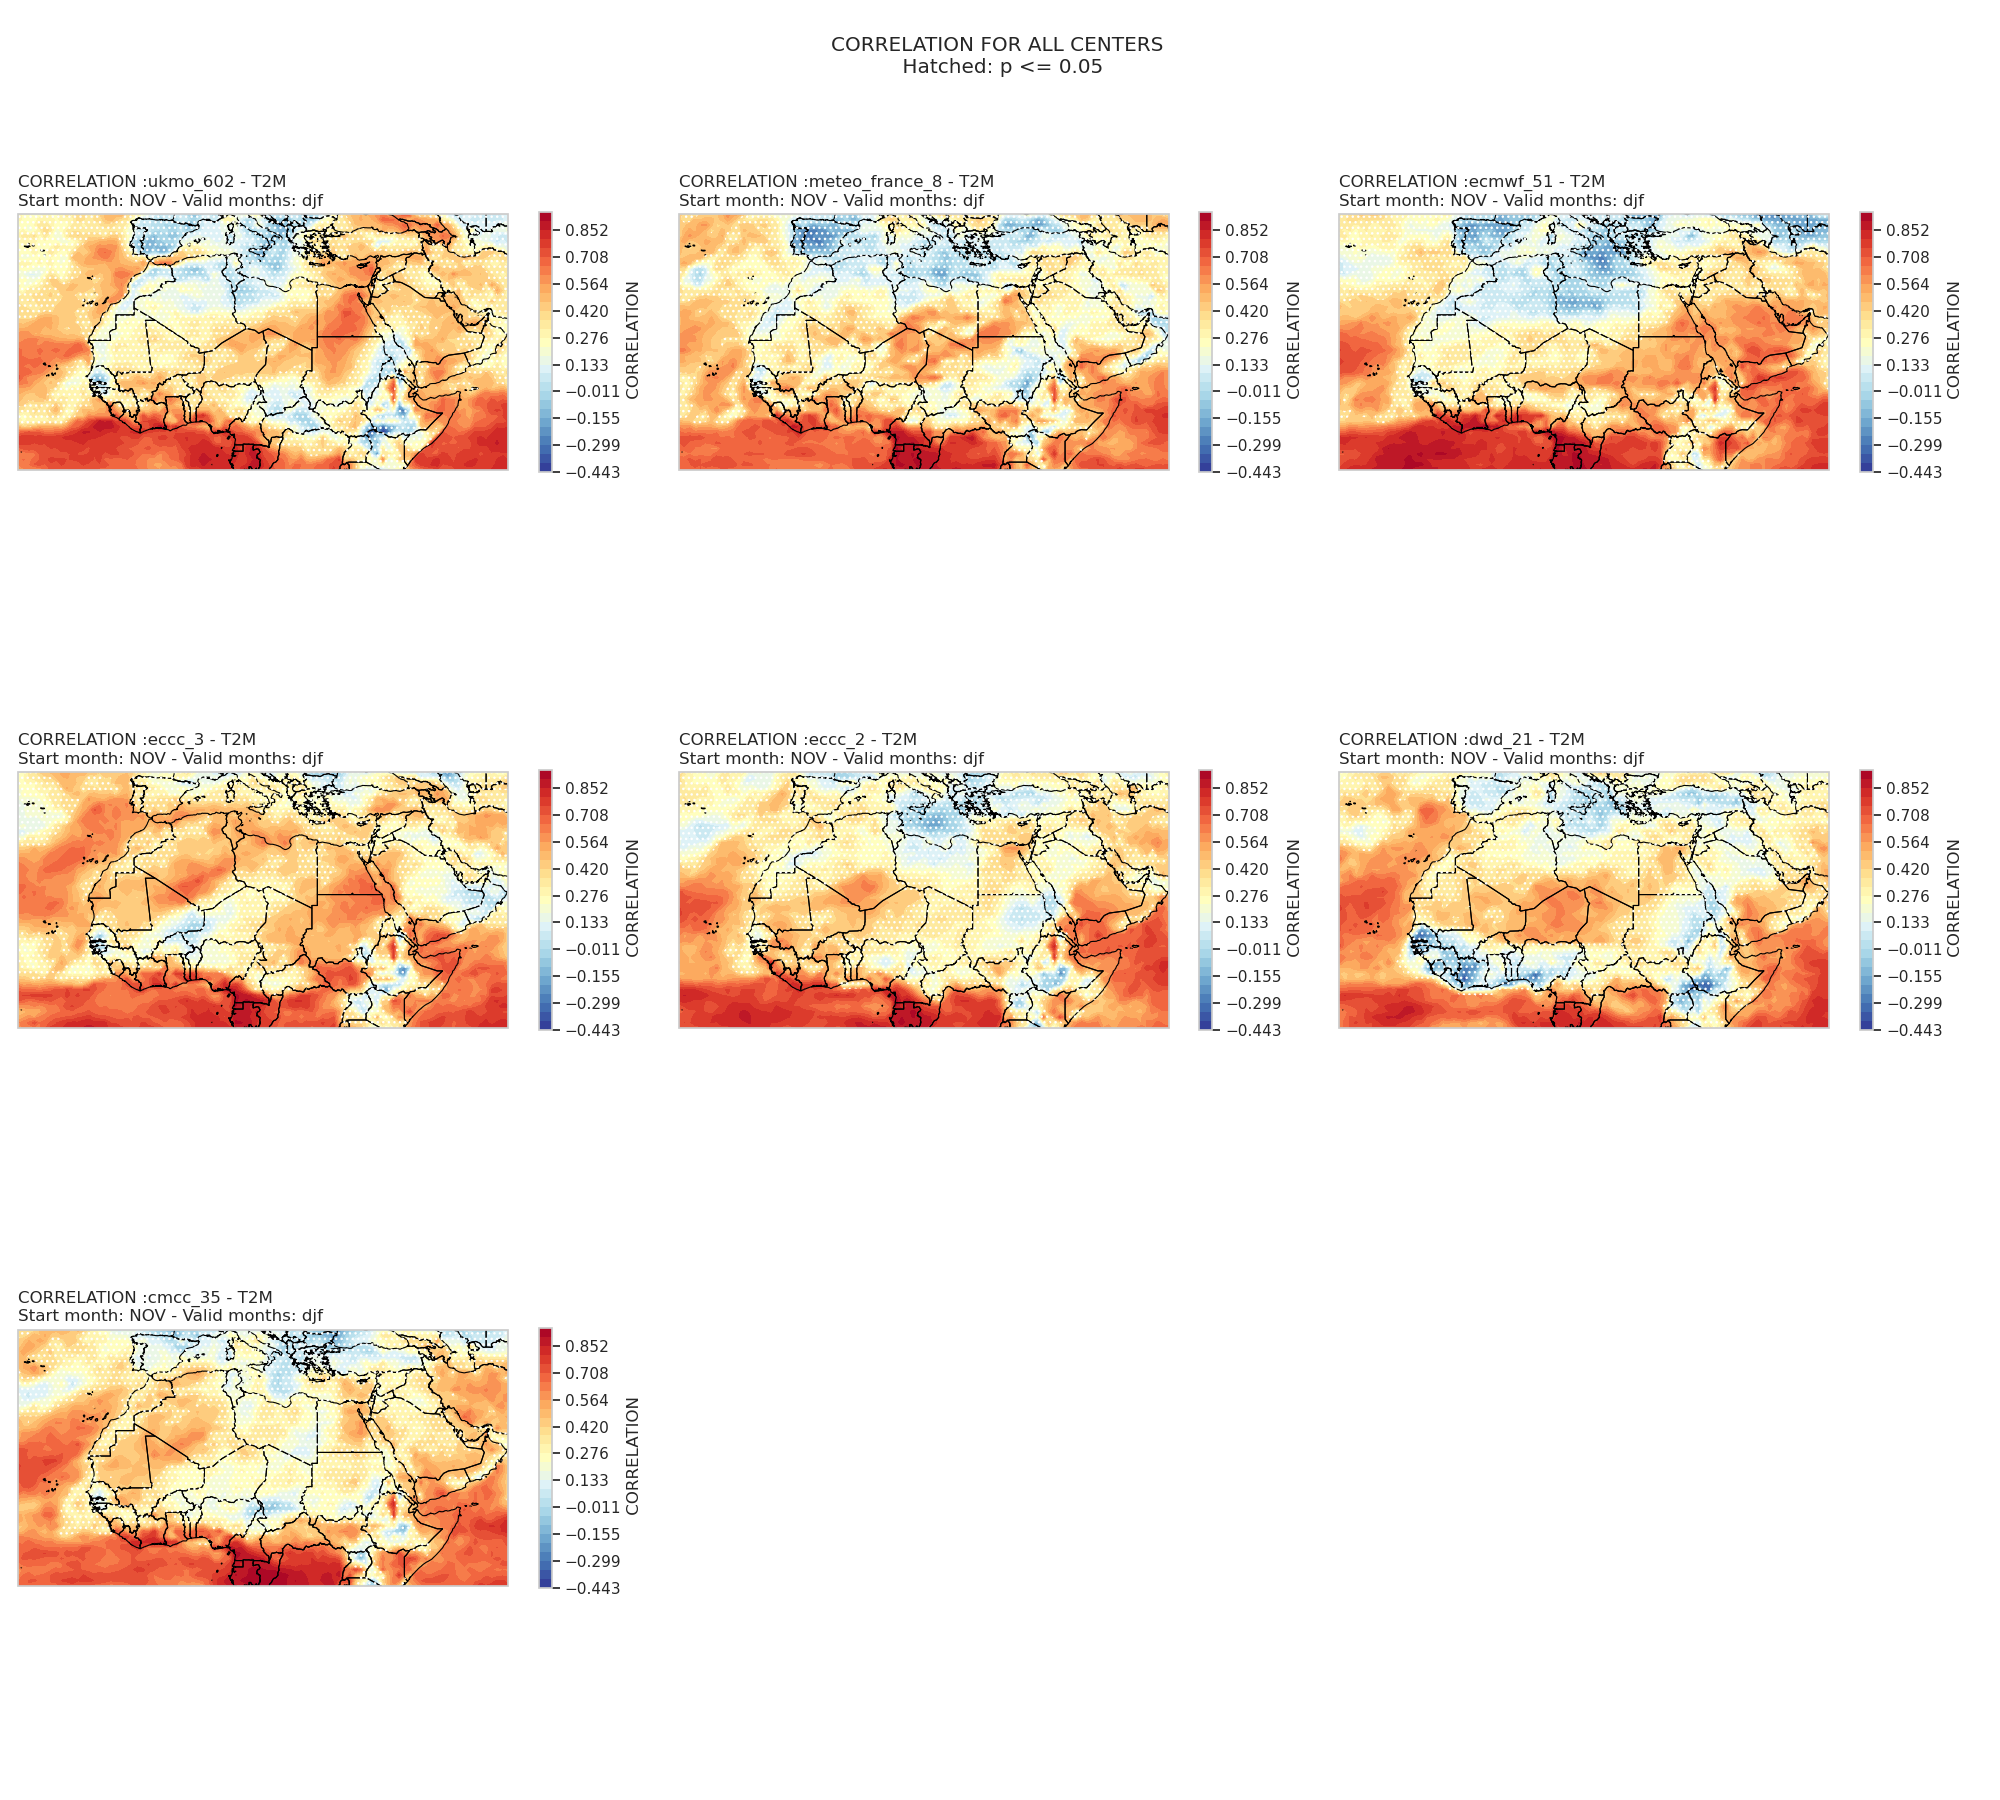
\includegraphics[width=1\linewidth]{plots/det/corr/CORR_djf_t2m.png}
    \caption{Temperature correlation maps for DJF (December-January-February)}
\end{figure}
The analysis of the \textbf{Spearman rank correlation for djf } from the figures above shows the following trends:

\begin{itemize}
    \item For the \textbf{UKMO model}, the correlation between observed and modeled temperatures is high (around 0.7) in southeastern Libya, Egypt, and northwestern Sudan. However, it is low and negative in Morocco, Algeria, and parts of Libya.
    \item The \textbf{Meteo-France model} exhibits a similar pattern, with high correlations in southeastern Libya and Egypt but low and negative values in Morocco and Algeria.
    \item In contrast, the \textbf{ECMWF model} shows higher correlations in Saudi Arabia and Yemen.
    \item For the \textbf{ECCC System 3 model}, the correlations are notably higher over a large part of the region, indicating better agreement between observed and modeled temperatures.
\end{itemize}
\begin{figure}[H]
    \centering
    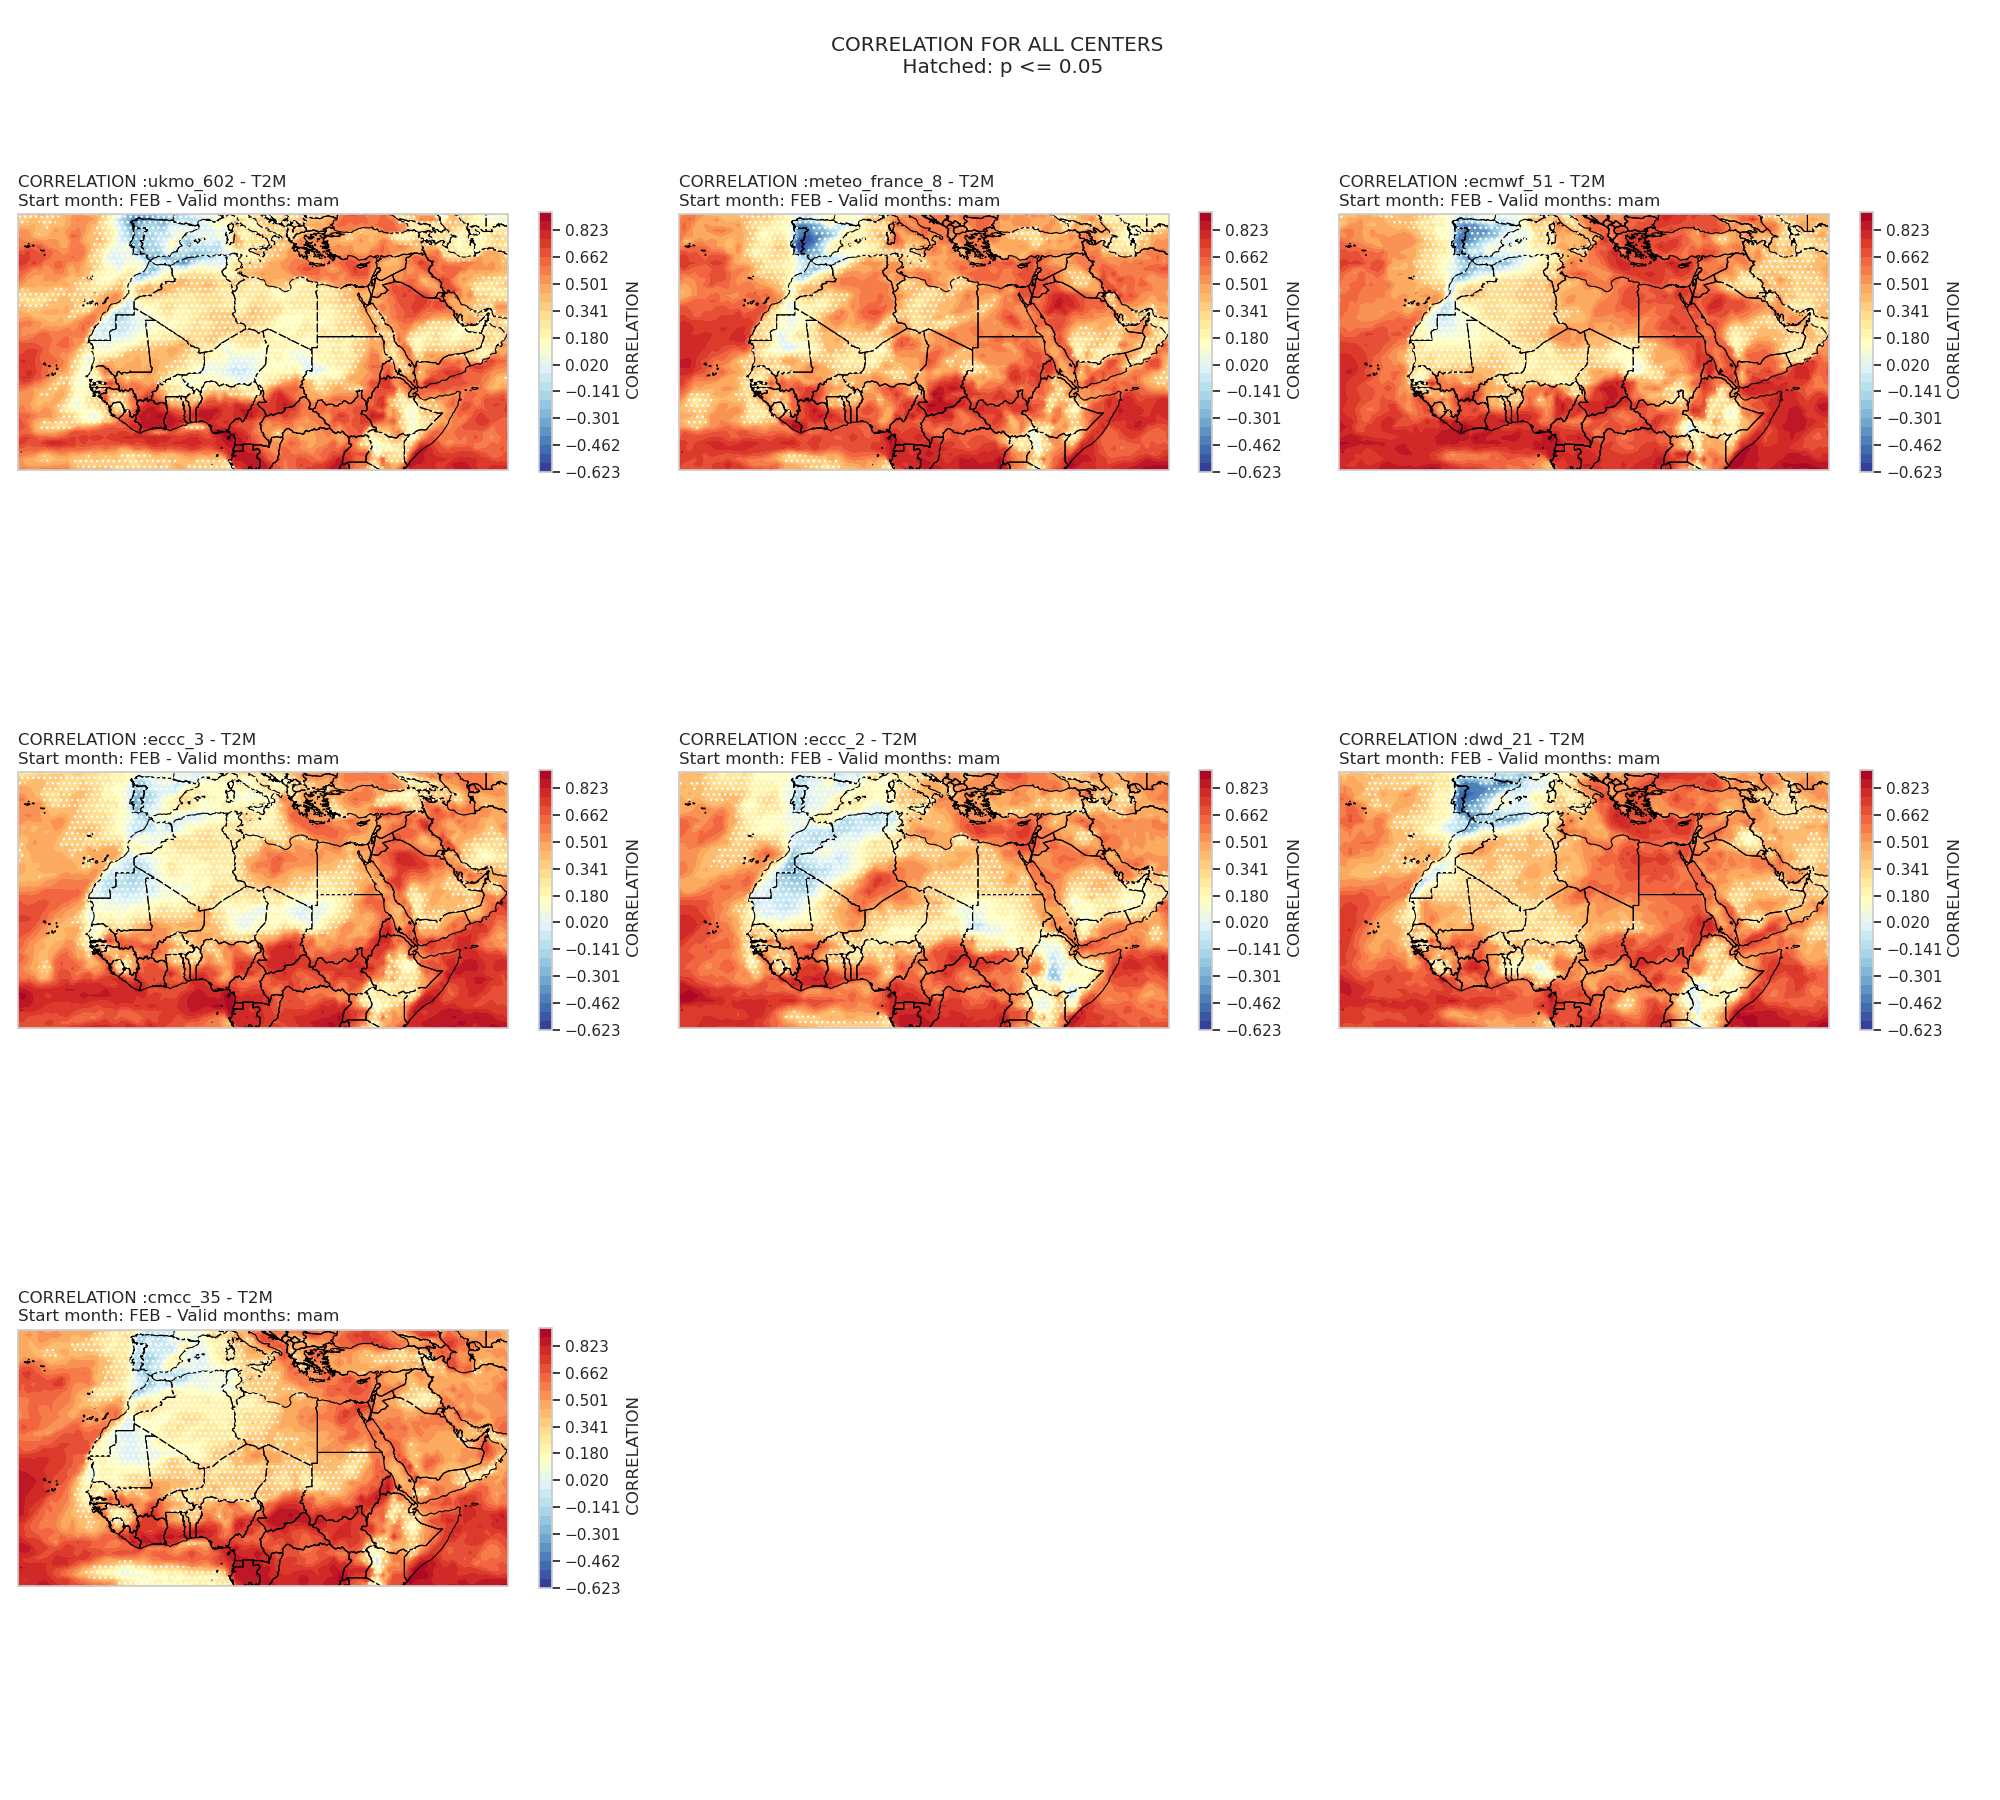
\includegraphics[width=1\linewidth]{plots/det/corr/CORR_mam_t2m.png}
    \caption{temperature correlation maps for mam}
\end{figure}
For MMA, the Met Office, ECMWF, and DWD demonstrate better performance across this region, except in northern Morocco, where correlations range between approximately -0.12 and 0.02.
\begin{figure}[H]
    \centering
    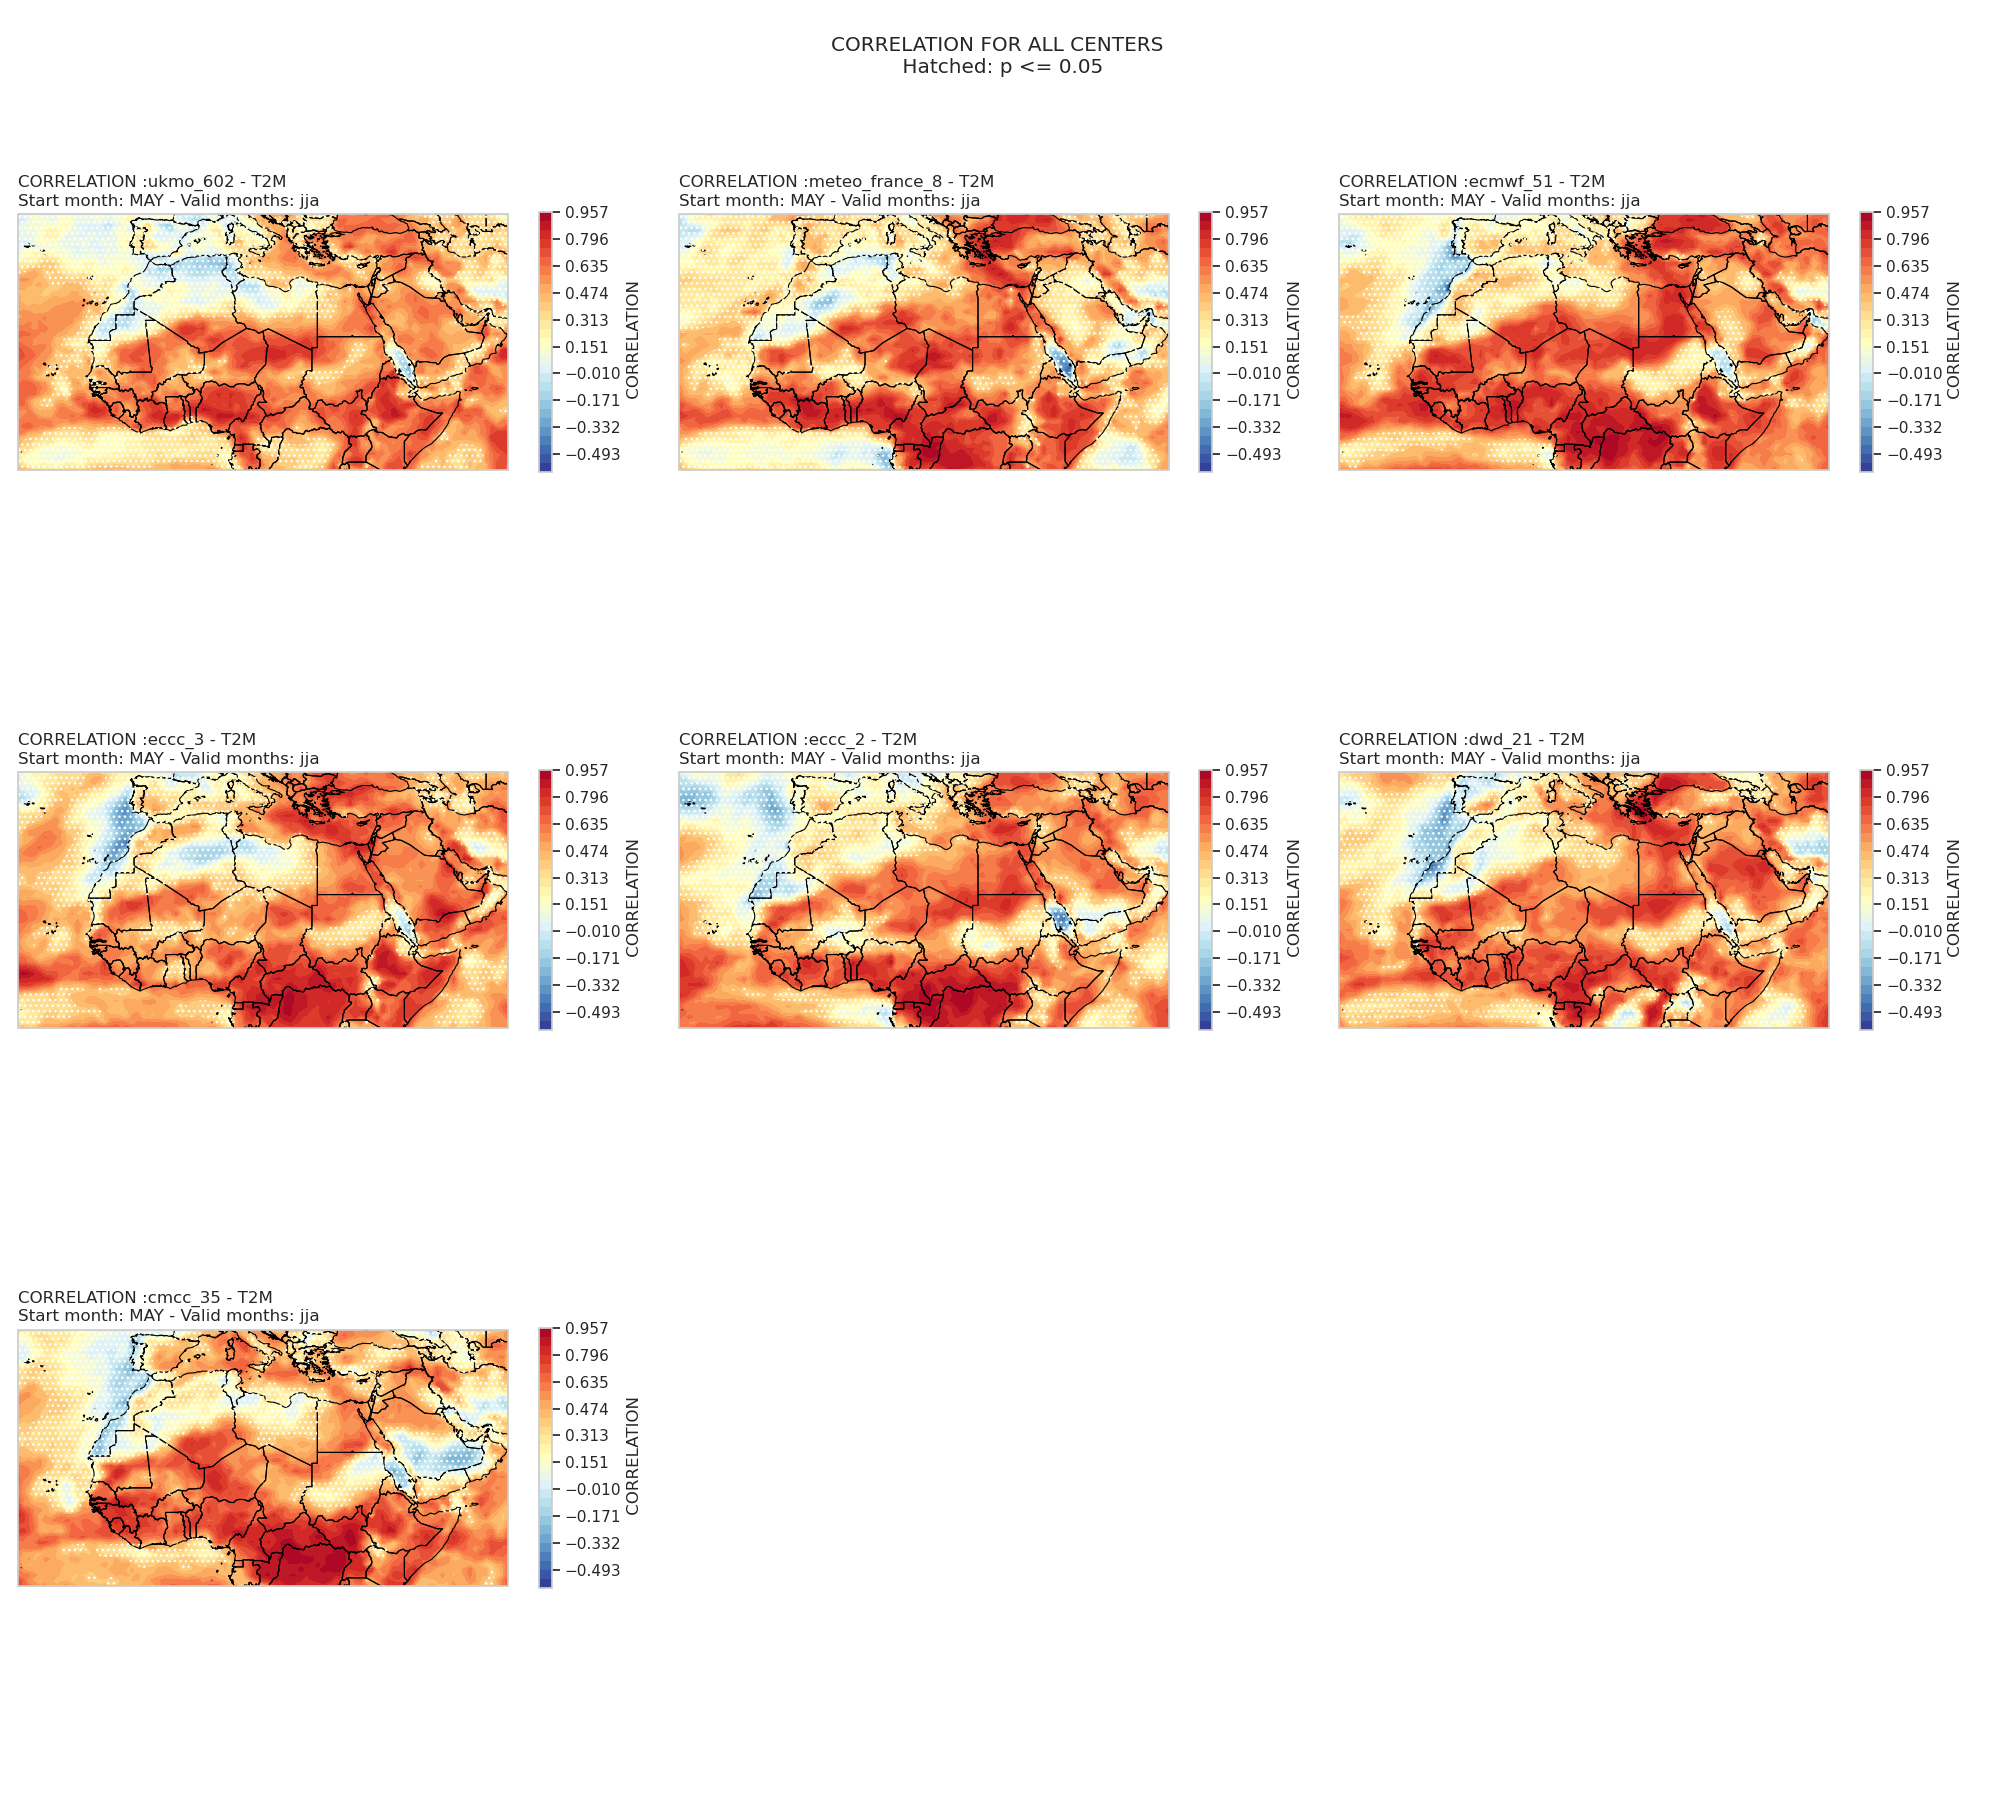
\includegraphics[width=1\linewidth]{plots/det/corr/CORR_jja_t2m.png}
    \caption{temperature correlation maps for jja}
   
\end{figure}
For JJA, the ECMWF and ECCC-2 models exhibit the best correlations overall, except in southern Morocco and Tunisia, where their performance is notably weaker.
\begin{figure}[H]
    \centering
    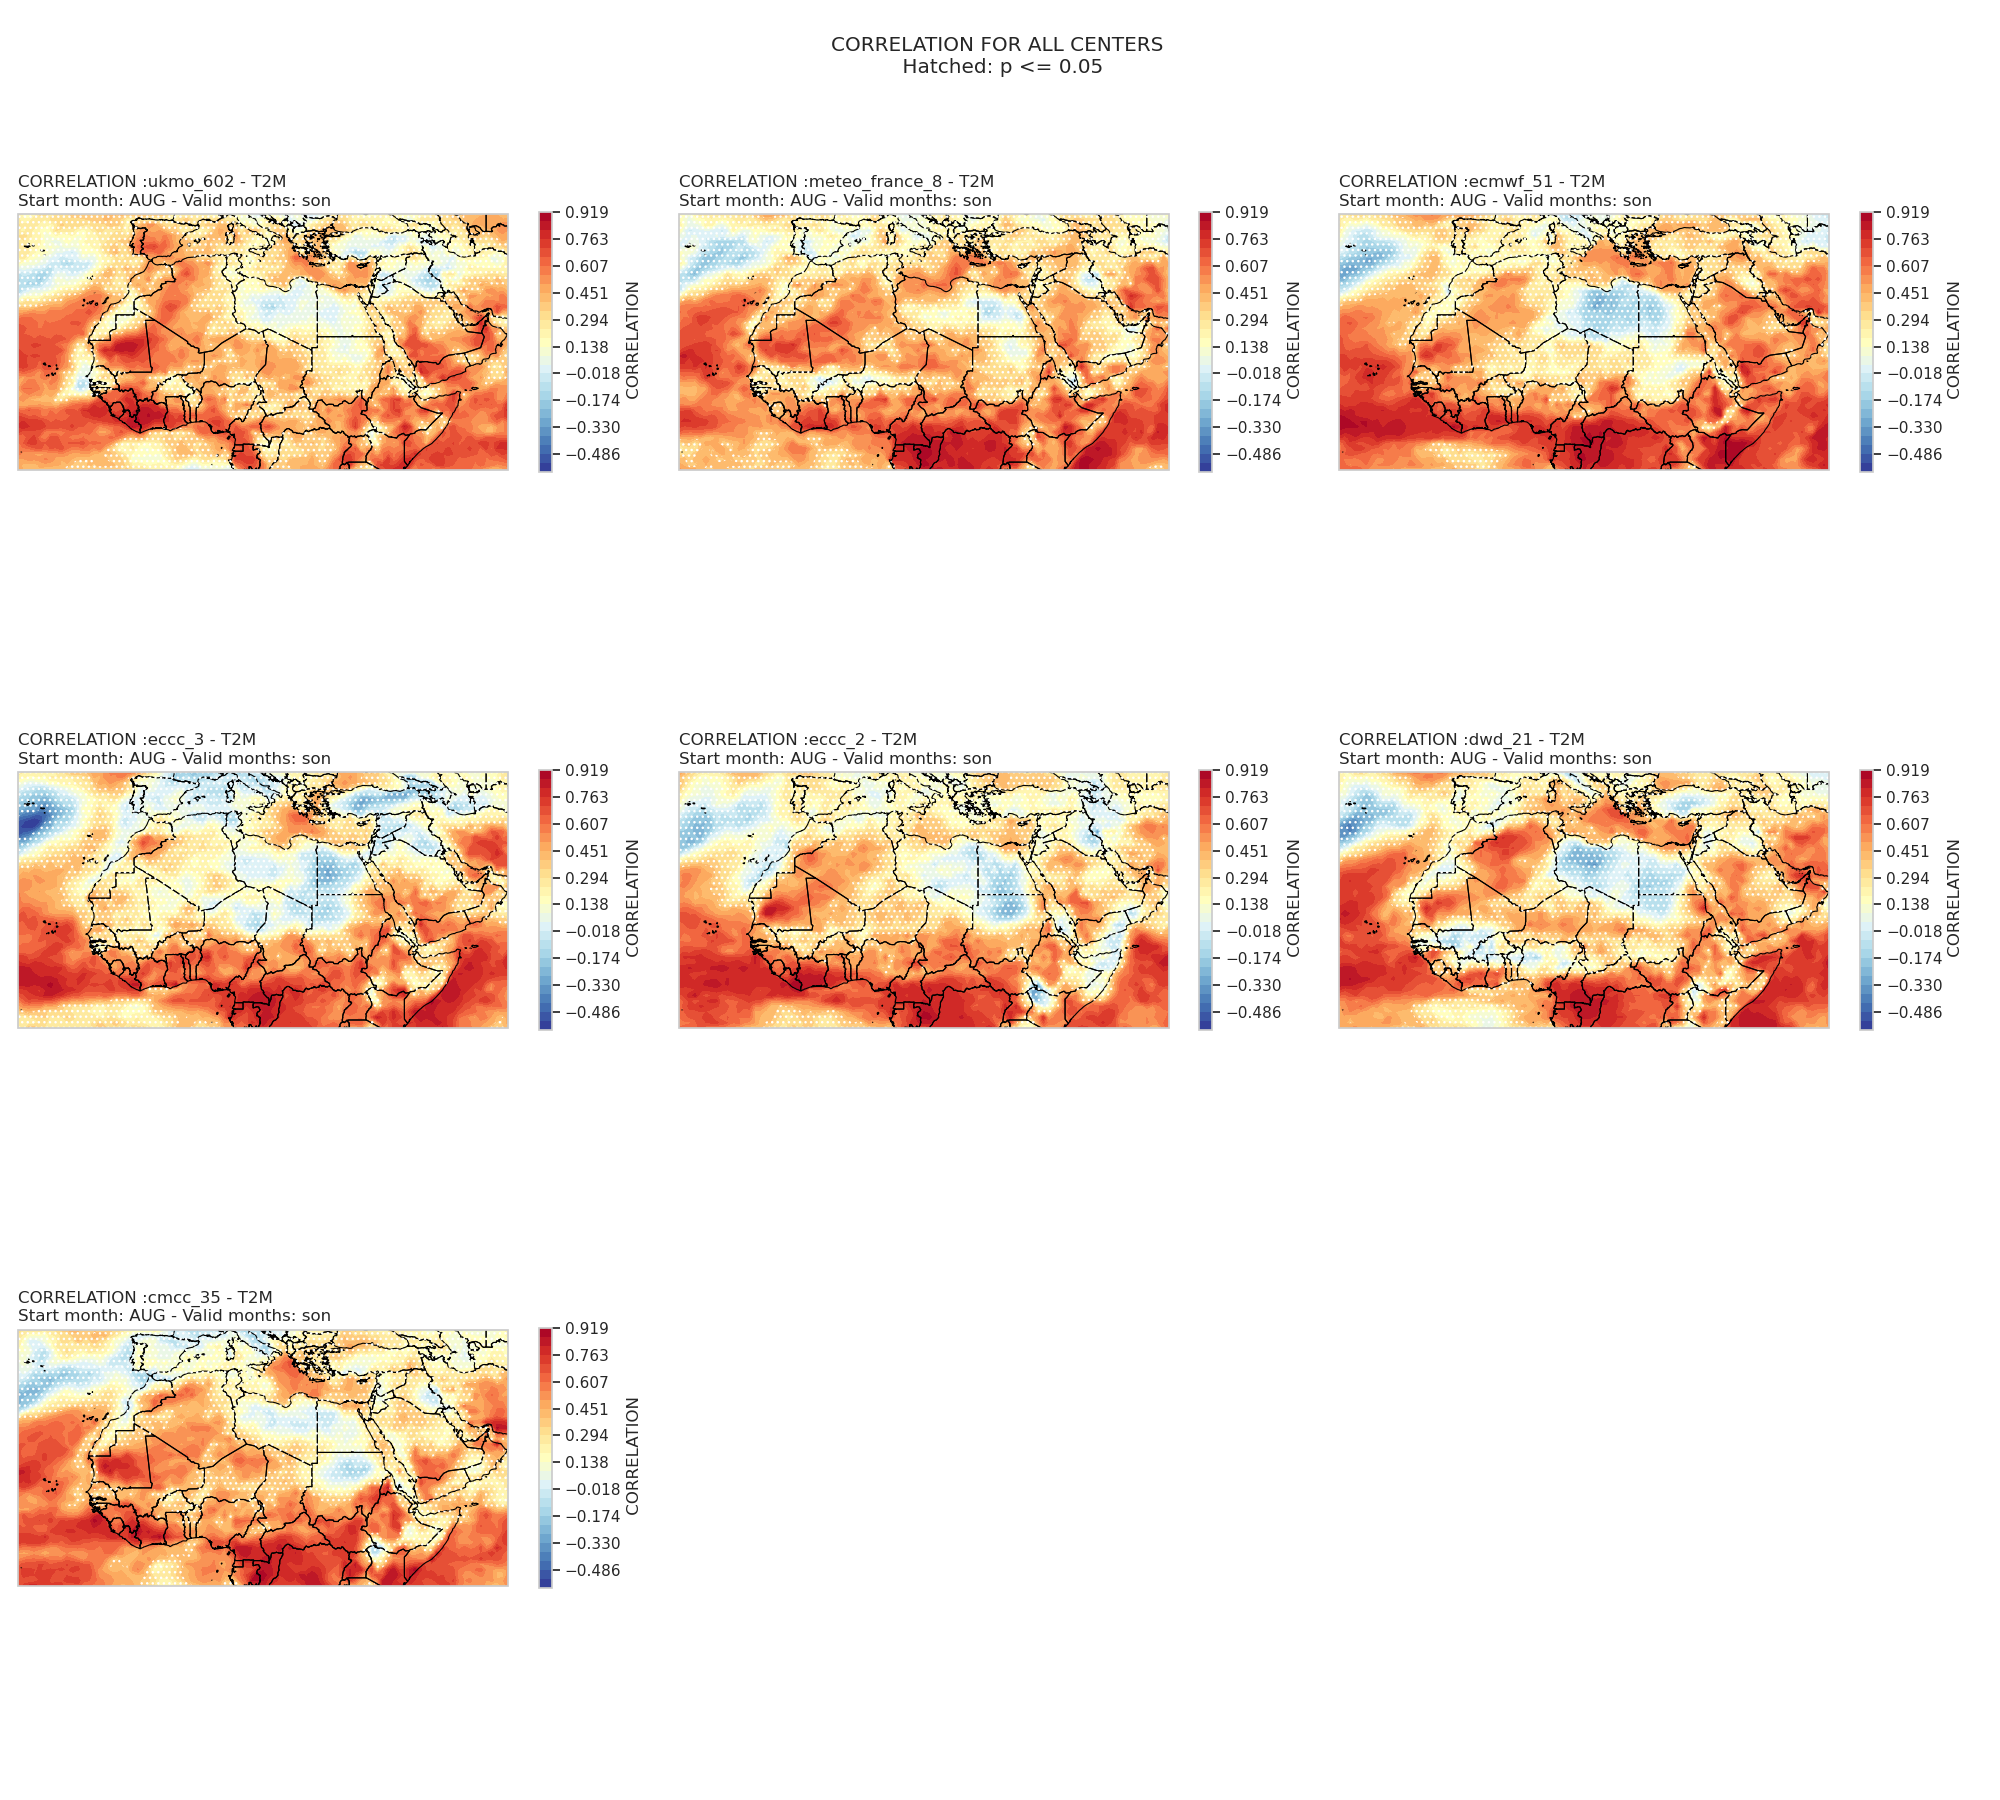
\includegraphics[width=1\linewidth]{plots/det/corr/CORR_son_t2m.png}
    \caption{temperature correlation maps for son}
   
\end{figure}
For SON , the Meteo-France model performs well, except in Egypt, showing better correlations in Morocco compared to other models and seasons. Similarly, the ECMWF model also performs well but shows weaker correlations in Libya and Egypt.
\begin{figure}[H]
    \centering
    \includegraphics[width=1\linewidth]{plots/det/corr/corr_T2M.png}
    \caption{Temperature heatmap for mena region}
   
\end{figure}


The heatmaps provide an average overview of the models' performance across the MENA region for a given season and a forecast lead time ranging from 1 to 3 months. In general, correlations tend to decrease as the lead time increases from 1 to 3 months. For instance, the ECMWF model shows higher performance during JJA, whereas the ECCC-2 model performs better during MAM. As previously mentioned, these results represent averages over the entire region. For a more detailed analysis, a mask was applied to focus specifically on North African countries within the MENA region. The results of this targeted analysis are shown in the heatmap below.
\begin{figure}[H]
    \centering
    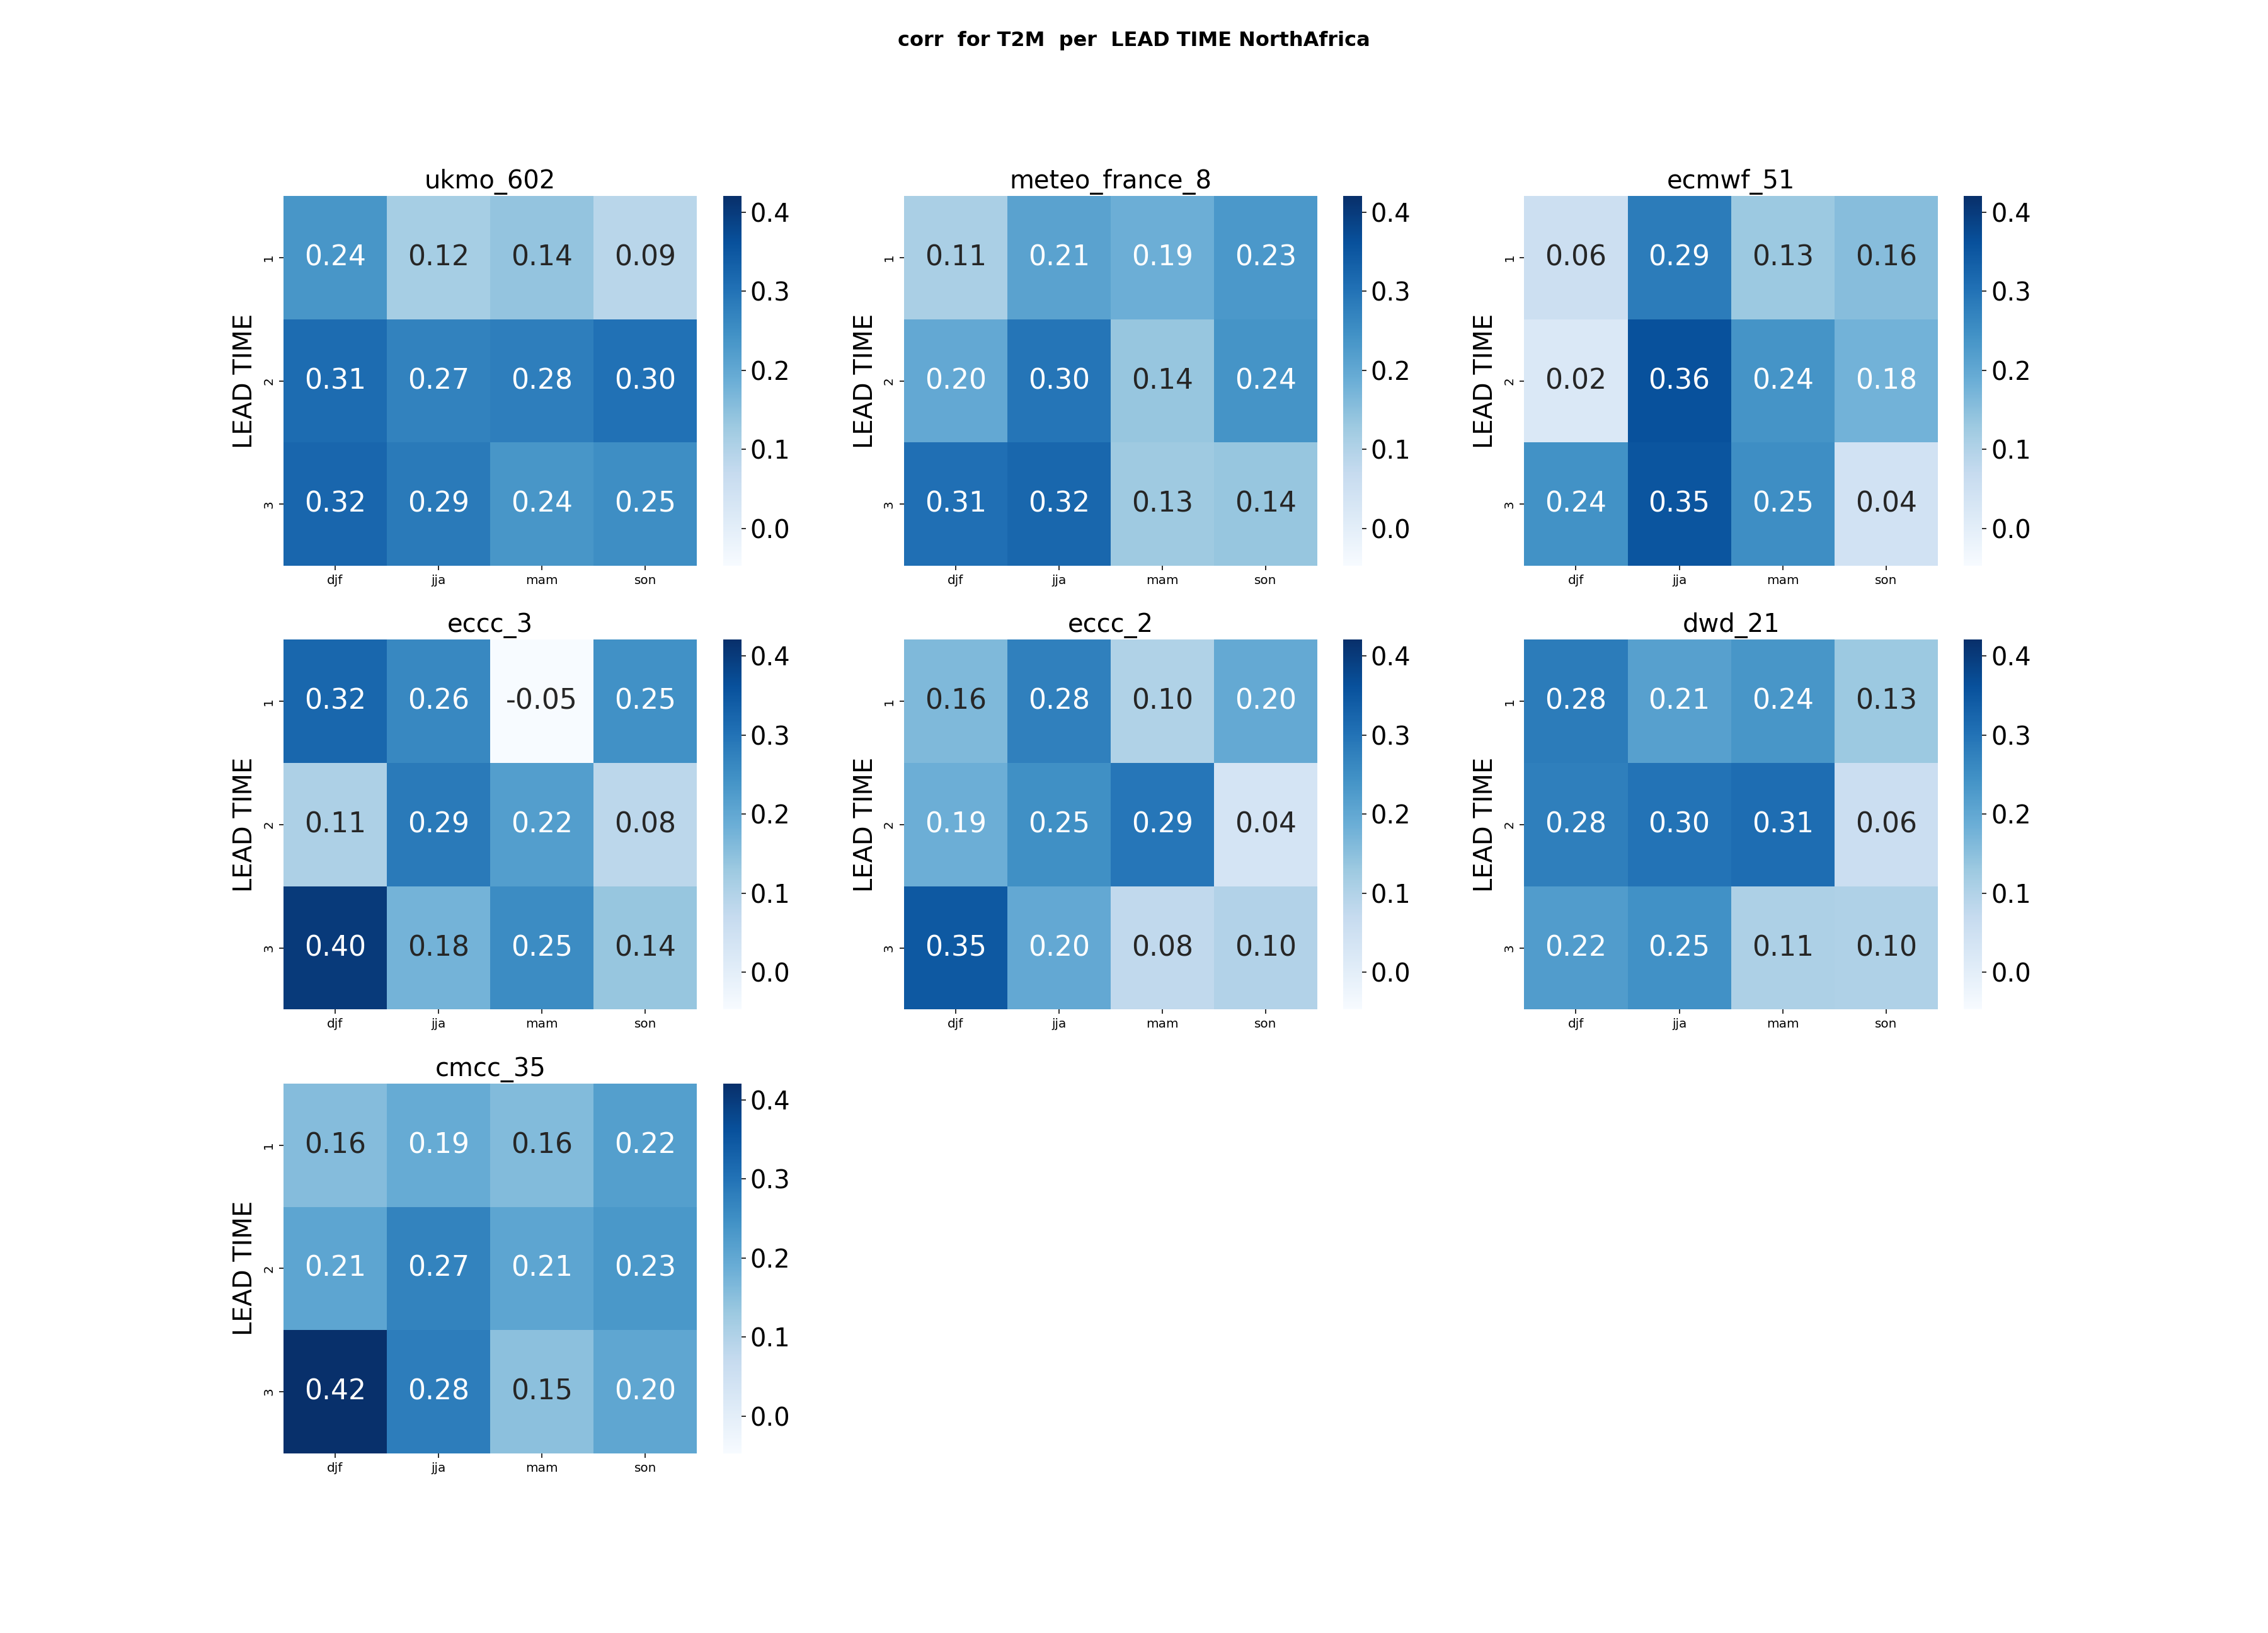
\includegraphics[width=1\linewidth]{plots/det/corr/corr_T2M_NorthAfrica.png}
    \caption{Temperature heatmap for north africa}
   
\end{figure}
\subsubsection{Root Mean Square Error}


The maps in this section show the RMSE (Root Mean Square Error) between observed and modeled surface temperatures across the MENA region for the four seasons: JJA, DJF, MAM, and SON. The RMSE, expressed in the same units as temperature, evaluates the accuracy of climate models, with lower values indicating better performance.  These maps help identify the strengths and limitations of the models across seasons, contributing to the improvement of climate forecasts for the region.
\begin{figure}[H]
    \centering
    \includegraphics[width=1\linewidth]{plots/det/rmse/rmse_T2M.png}
    \caption{Temperature rmse heatmaps for all the sasons}
\end{figure}

The heatmap for the seven models highlights distinct variations in their seasonal performance. The UKMO model shows moderate to good performance, particularly in JJA and MAM, as reflected by relatively low RMSE values ranging between 1.35°C and 1.51°C across the three lead times. This indicates that the UKMO model is reasonably effective in capturing surface temperature variations during these seasons, likely benefiting from its ability to simulate key atmospheric processes during these periods.

In contrast, Météo-France exhibits weaker performance in JJA, with higher RMSE values suggesting less accurate predictions of surface temperatures during this season. This could be attributed to the model's limitations in capturing summer-specific temperature drivers in the MENA region, such as heatwaves, desert-air interactions, or seasonal atmospheric circulation patterns.

The ECMWF model emerges as the best-performing model based on the heatmap, particularly during JJA, where it demonstrates high predictive accuracy and consistency. This is supported by the RMSE map, which shows significantly lower RMSE values across most of the MENA region. These low RMSE values confirm the ECMWF model's ability to capture regional temperature dynamics effectively, with reduced errors across diverse climatic zones.

Notably, the spatial distribution of RMSE on the map reinforces the ECMWF's strong performance, as it maintains relatively low error values in critical parts of the MENA region. This suggests that the ECMWF model is better equipped to account for the complex climatic interactions in the region, such as the influence of desert regions, coastal temperature gradients, and seasonal weather patterns.

Overall, these findings emphasize the importance of selecting climate models based on their seasonal and spatial performance, as they play a critical role in improving the accuracy of temperature forecasts for the MENA region.

\begin{figure}[H]
    \centering
    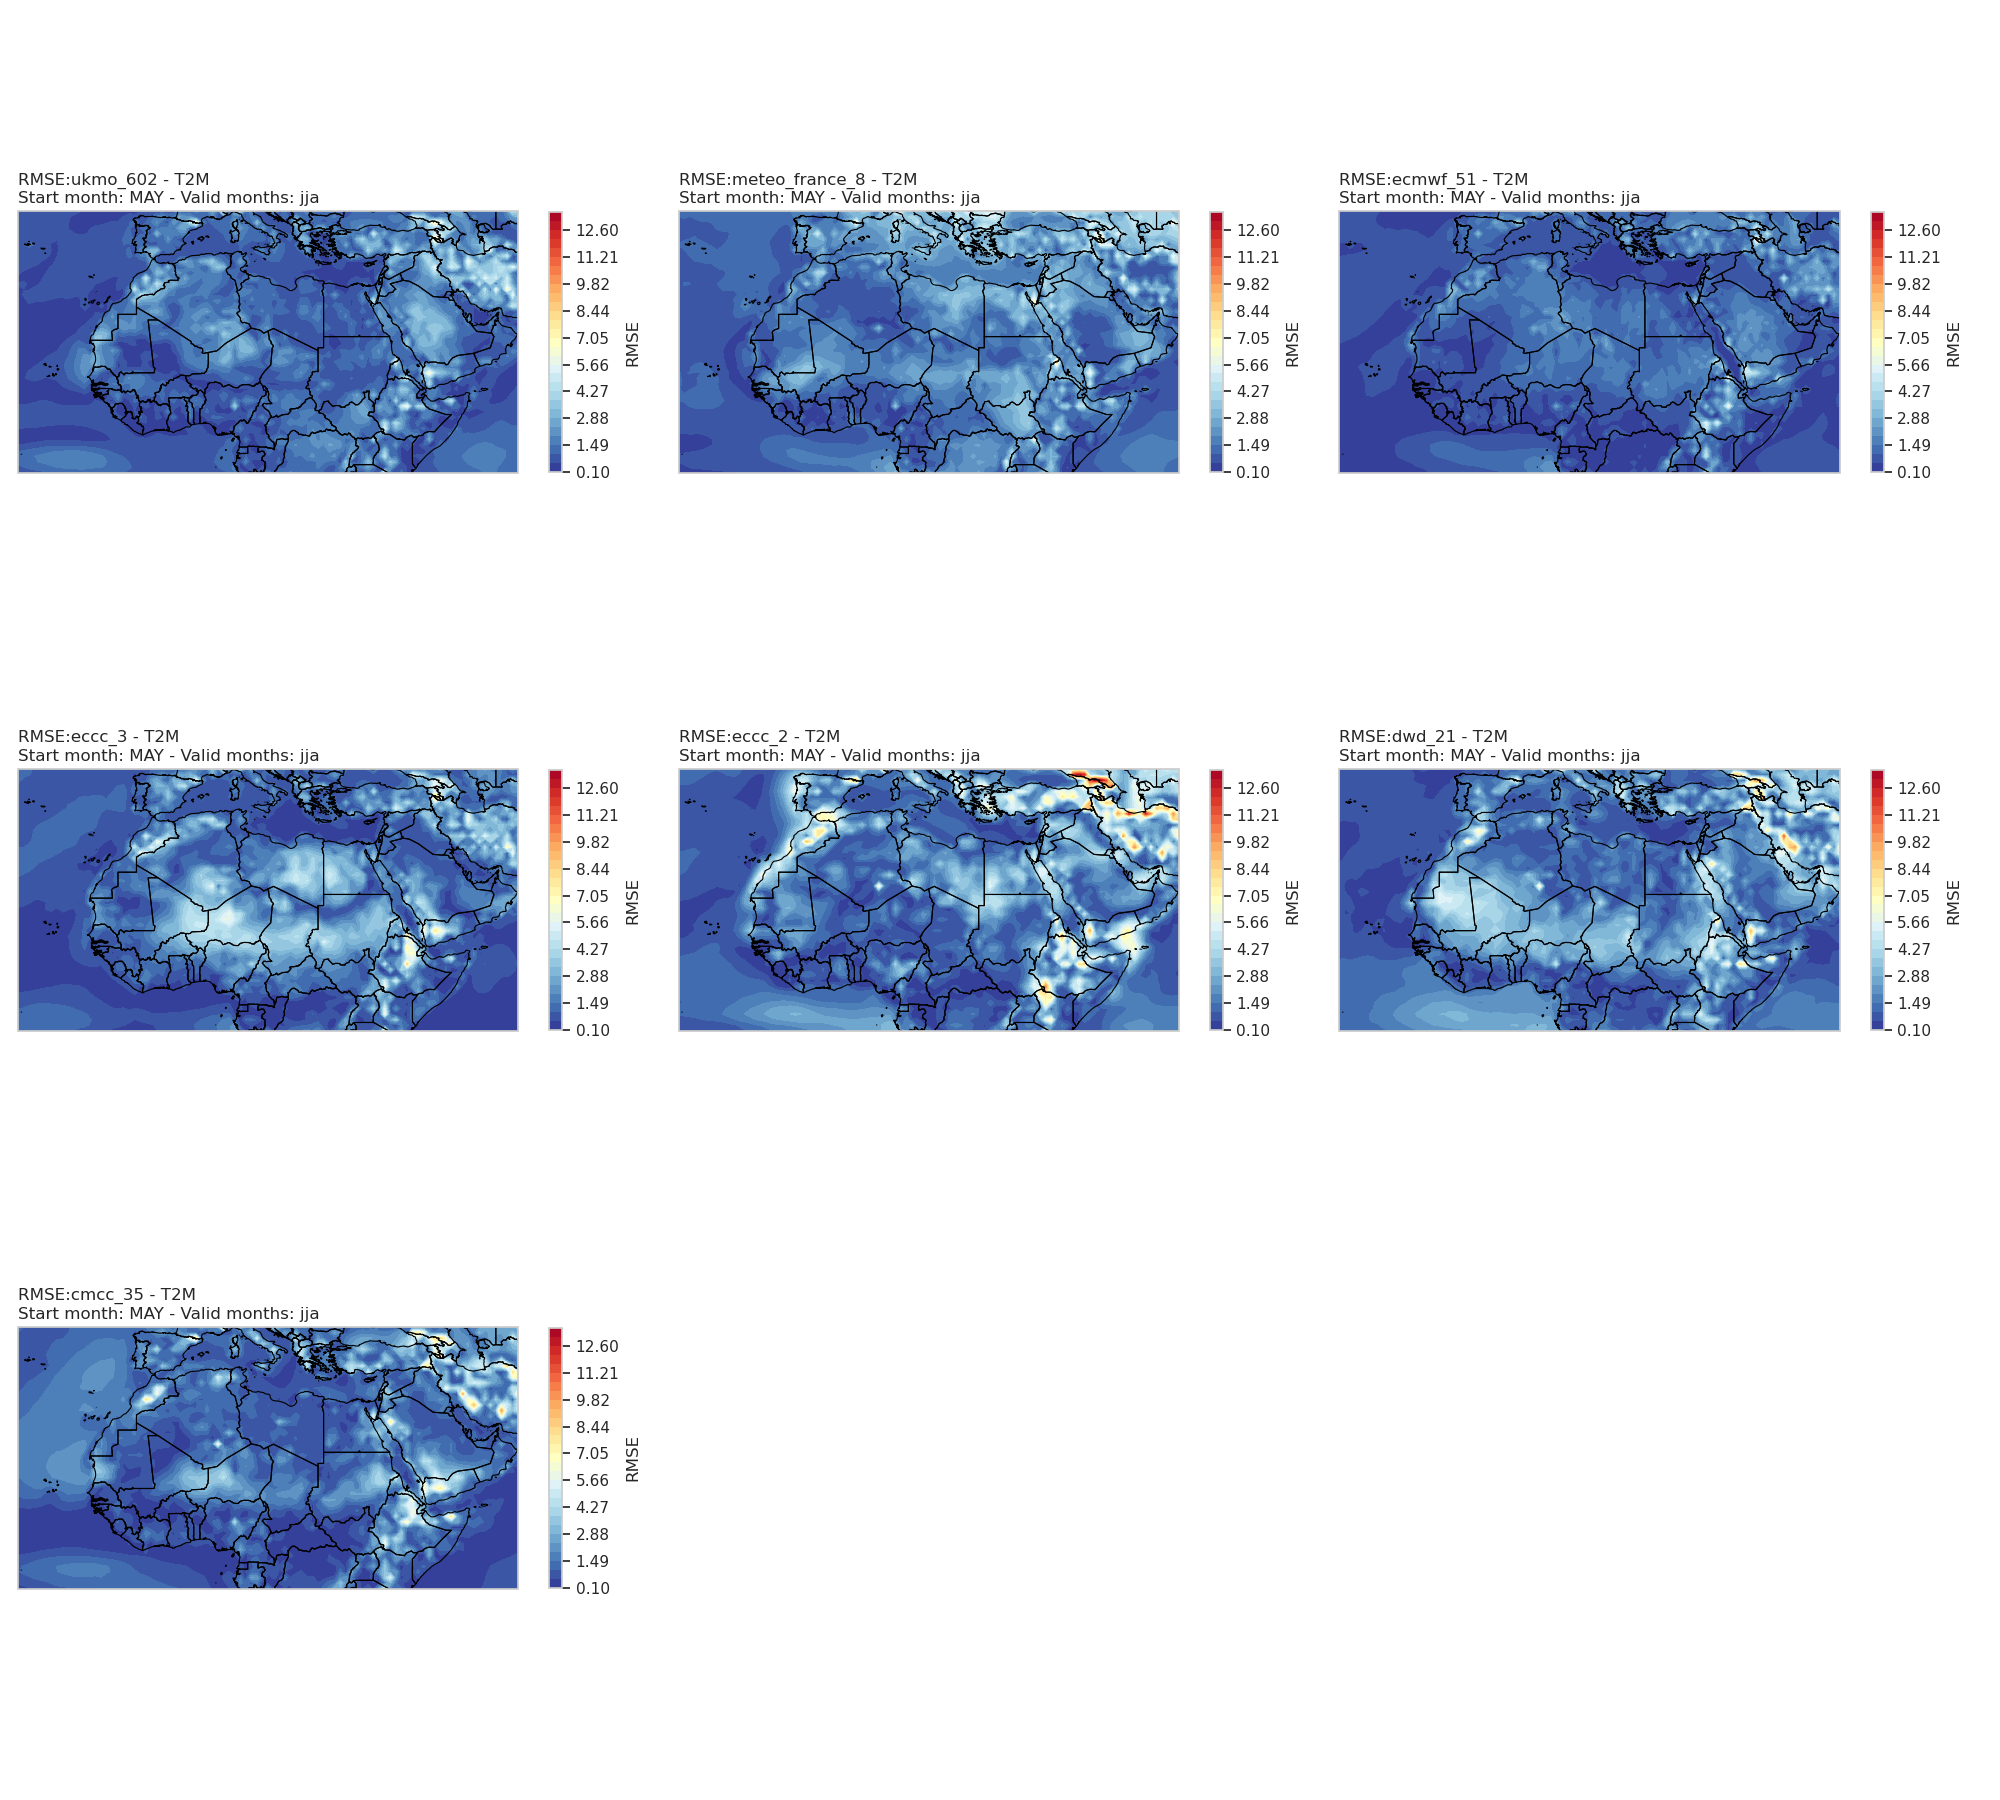
\includegraphics[width=1\linewidth]{plots/det/rmse/rmse_jja_t2m.png}
    \caption{temperature rmse maps for jja}
\end{figure}
To better understand the performance of climate models in sub-regions of MENA, a focus on North Africa is essential due to its distinct climatic features, such as vast desert landscapes, high seasonal temperature variability, and localized weather phenomena. The heatmap provides a comparative analysis of RMSE values for the seven models across this region, highlighting their seasonal accuracy in predicting surface temperatures.

The North African climate, heavily influenced by the Sahara Desert and Mediterranean coast, presents unique challenges for climate modeling, such as accurately simulating extreme temperatures and their spatial distribution. By examining the heatmap, we can identify which models perform well in capturing these specific climatic patterns and assess their suitability for seasonal forecasting in this critical sub-region of MENA.
\begin{figure}[H]
    \centering
    \includegraphics[width=1\linewidth]{plots/det/rmse/rmse_T2M_NorthAfrica.png}
    \caption{Temperature heatmap for north africa}
   
\end{figure}
This specific analysis revealed that, although the ECMWF model performs well across the MENA region, its performance in North Africa is comparatively lower, except during JJA. As highlighted earlier, JJA remains the most accurate season for ECMWF in this sub-region, with RMSE values ranging between 1.34°C and 1.58°C. This indicates that the model effectively captures temperature dynamics in the summer, likely due to its ability to simulate key seasonal factors such as strong solar heating and atmospheric circulation patterns specific to North Africa during this period.

In contrast, Météo-France demonstrates consistent performance across the three lead times and, on average, performs well over the four seasons in North Africa, particularly during SON. This could be attributed to the model’s ability to account for transitional weather conditions in autumn, such as changes in atmospheric pressure systems and coastal influences that significantly impact temperatures in this region.

These observations underline the importance of analyzing sub-regional performance to identify models that are better suited for specific areas and seasons. While ECMWF excels in JJA, Météo-France shows a more balanced performance throughout the year, making it potentially more reliable for multi-seasonal forecasting in North Africa.





\subsubsection{Coefficient of Determination (\( R^2 \))}
The maps in this section show the R-SQUARED between observed and modeled surface temperatures across the MENA region for the four seasons: JJA, DJF, MAM, and SON. R-SQUARED is a statistical measure that indicates how well the model explains the variability in observed data, with values closer to 1 signifying better performance. These maps provide valuable insights into the predictive skill of the climate models, highlighting their ability to capture seasonal temperature patterns.

\begin{figure}[H]
    \centering
    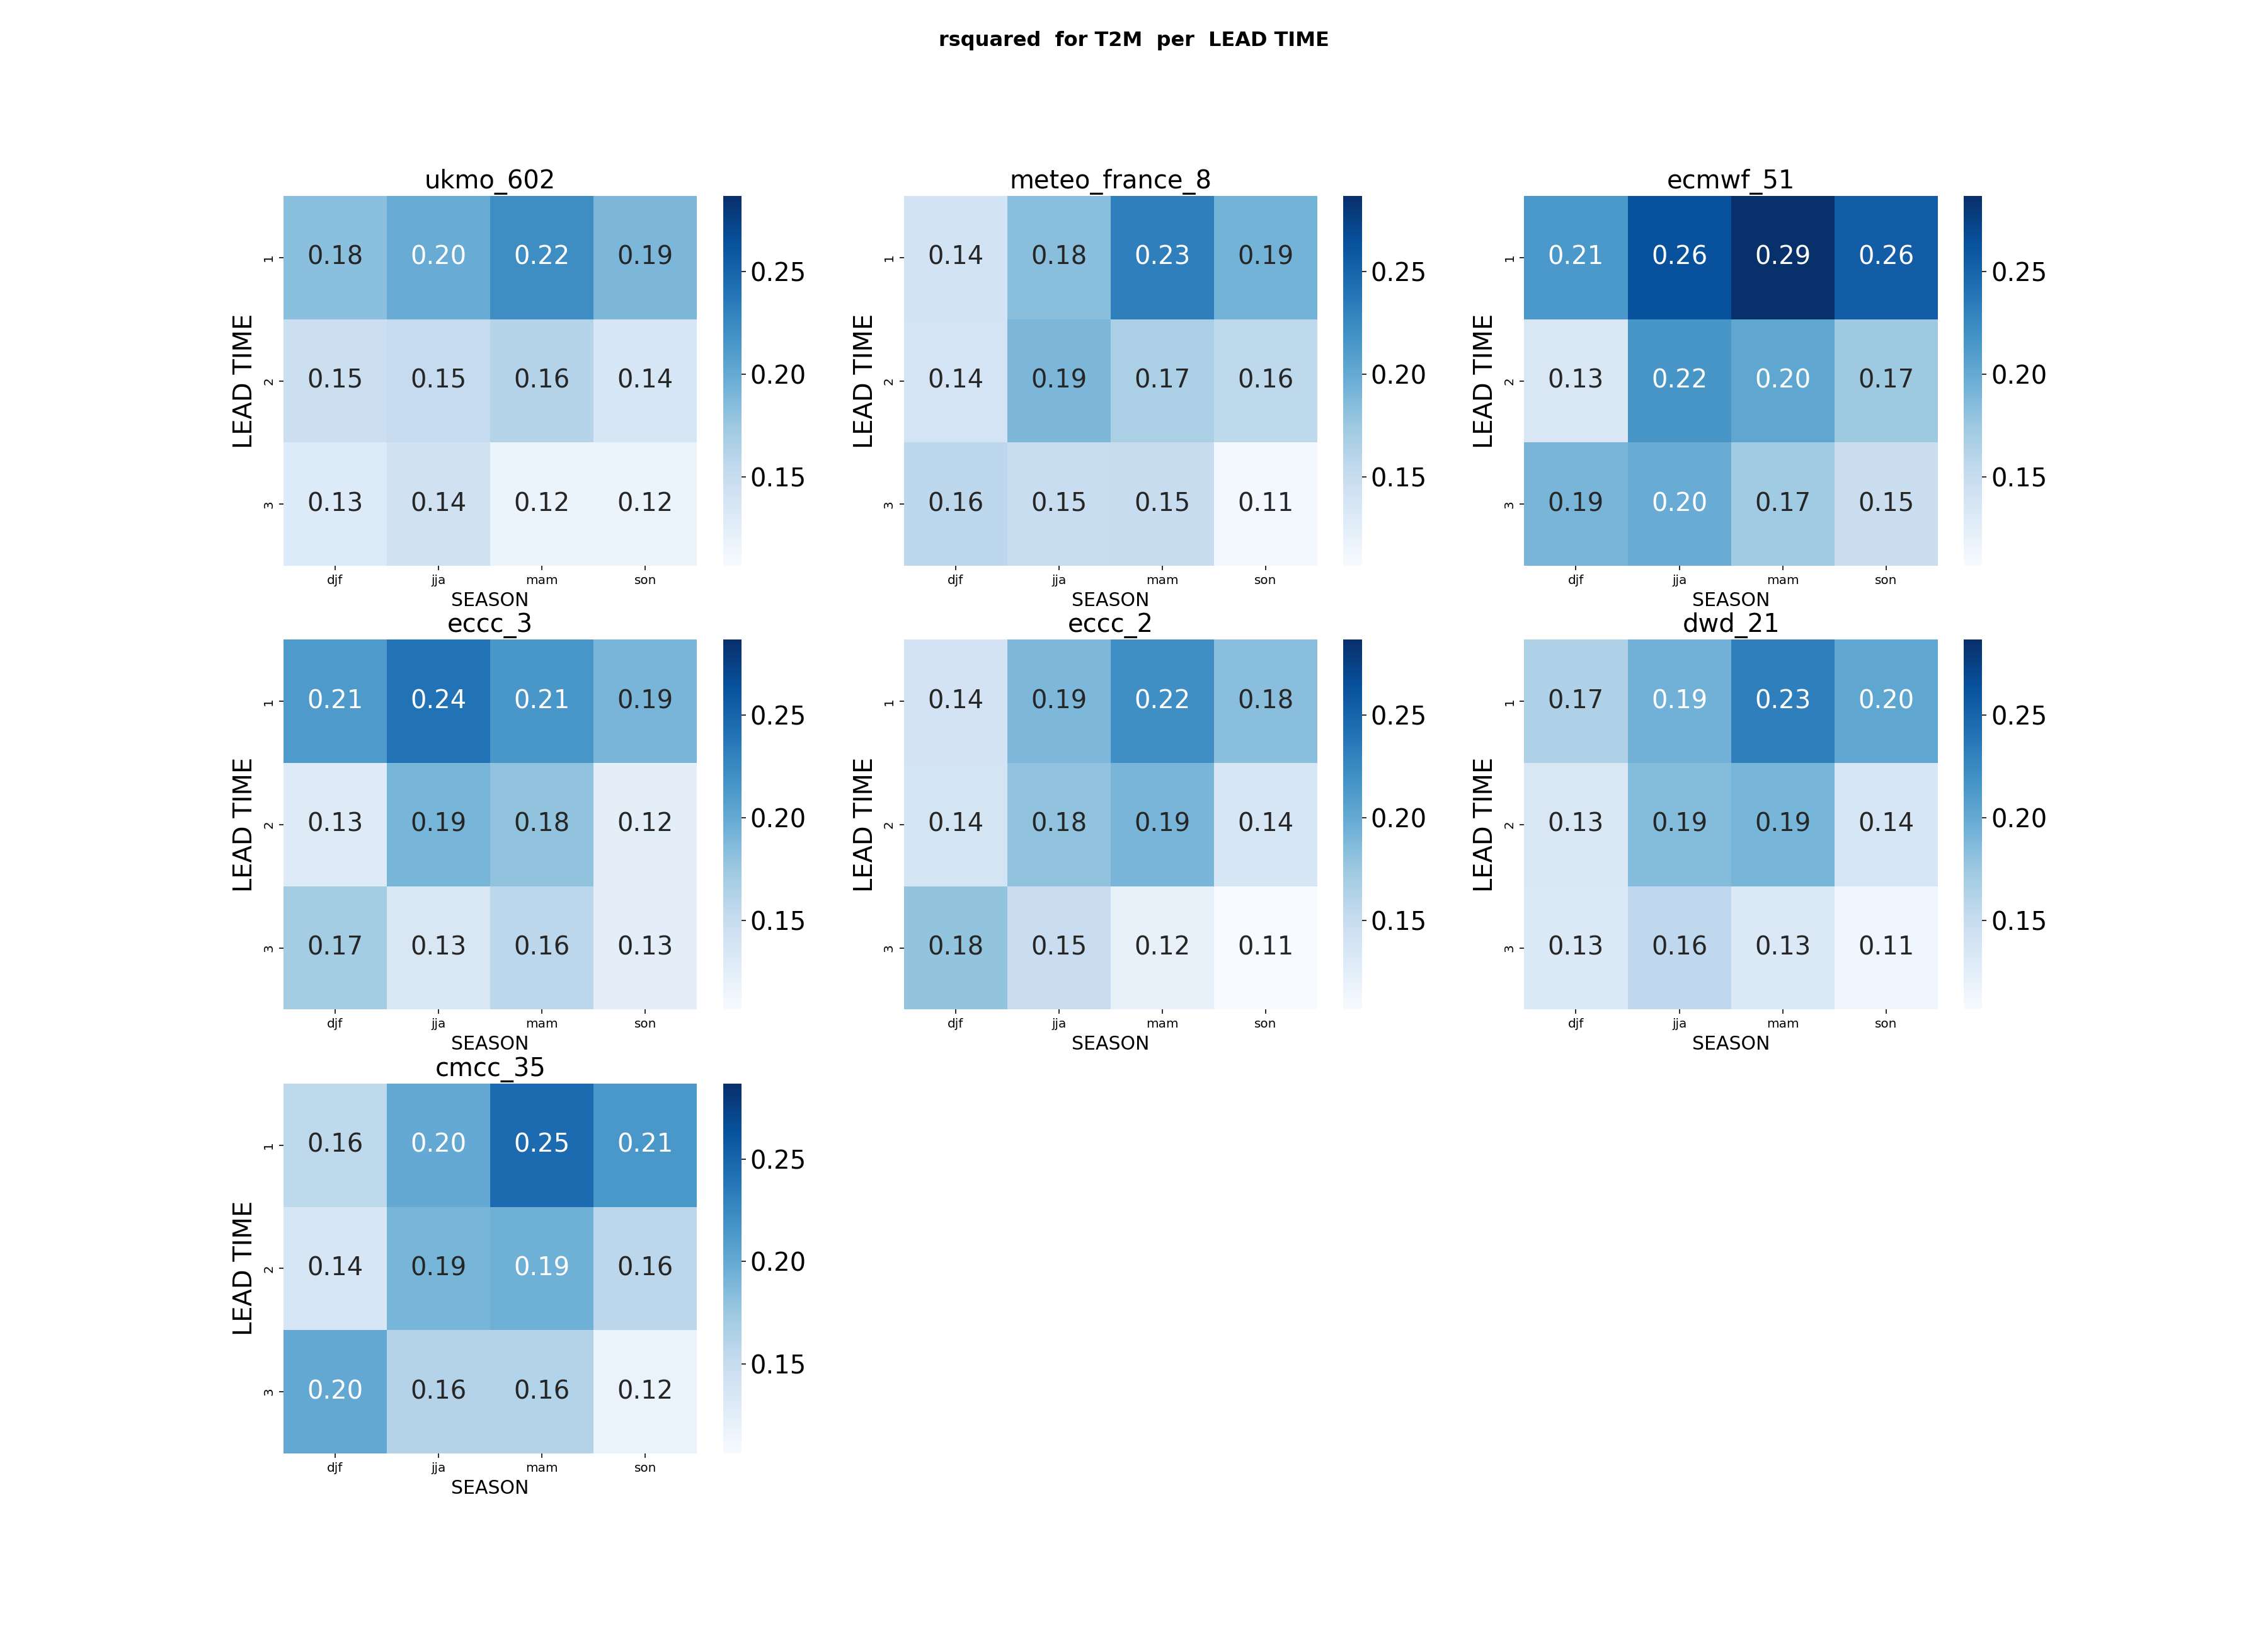
\includegraphics[width=1\linewidth]{plots/det/rsquared/rsquared_T2M.png}
    \caption{Temperature rsquared heatmaps for all the seasons}
\end{figure}

Based on this deterministic metric (R-SQUARED), the ECMWF model demonstrates superior performance for lead time 1 across all four seasons, particularly during MAM. In general, the portion of variance explained by the model decreases as the lead time increases. This indicates that while the model is highly effective at capturing seasonal variability of surface temperatures in the short term, its predictive skill diminishes over longer time horizons.

The strong performance during MAM highlights the ECMWF ability to capture the complexities of spring, a season marked by transitional weather patterns in the MENA region. The high R-SQUARED values during this period suggest that the model accurately reflects observed temperature variability by effectively simulating key drivers such as the gradual warming trend, atmospheric circulation changes, and the interaction between desert and coastal dynamics.

Such precision underscores the ECMWF model's reliability for short-term seasonal forecasting, particularly during periods of heightened climatic variability like MAM. However, the decreasing performance with increasing lead times suggests the need for careful interpretation of forecasts beyond lead time 1, as uncertainty increases with longer projections.

\begin{figure}[H]
    \centering
    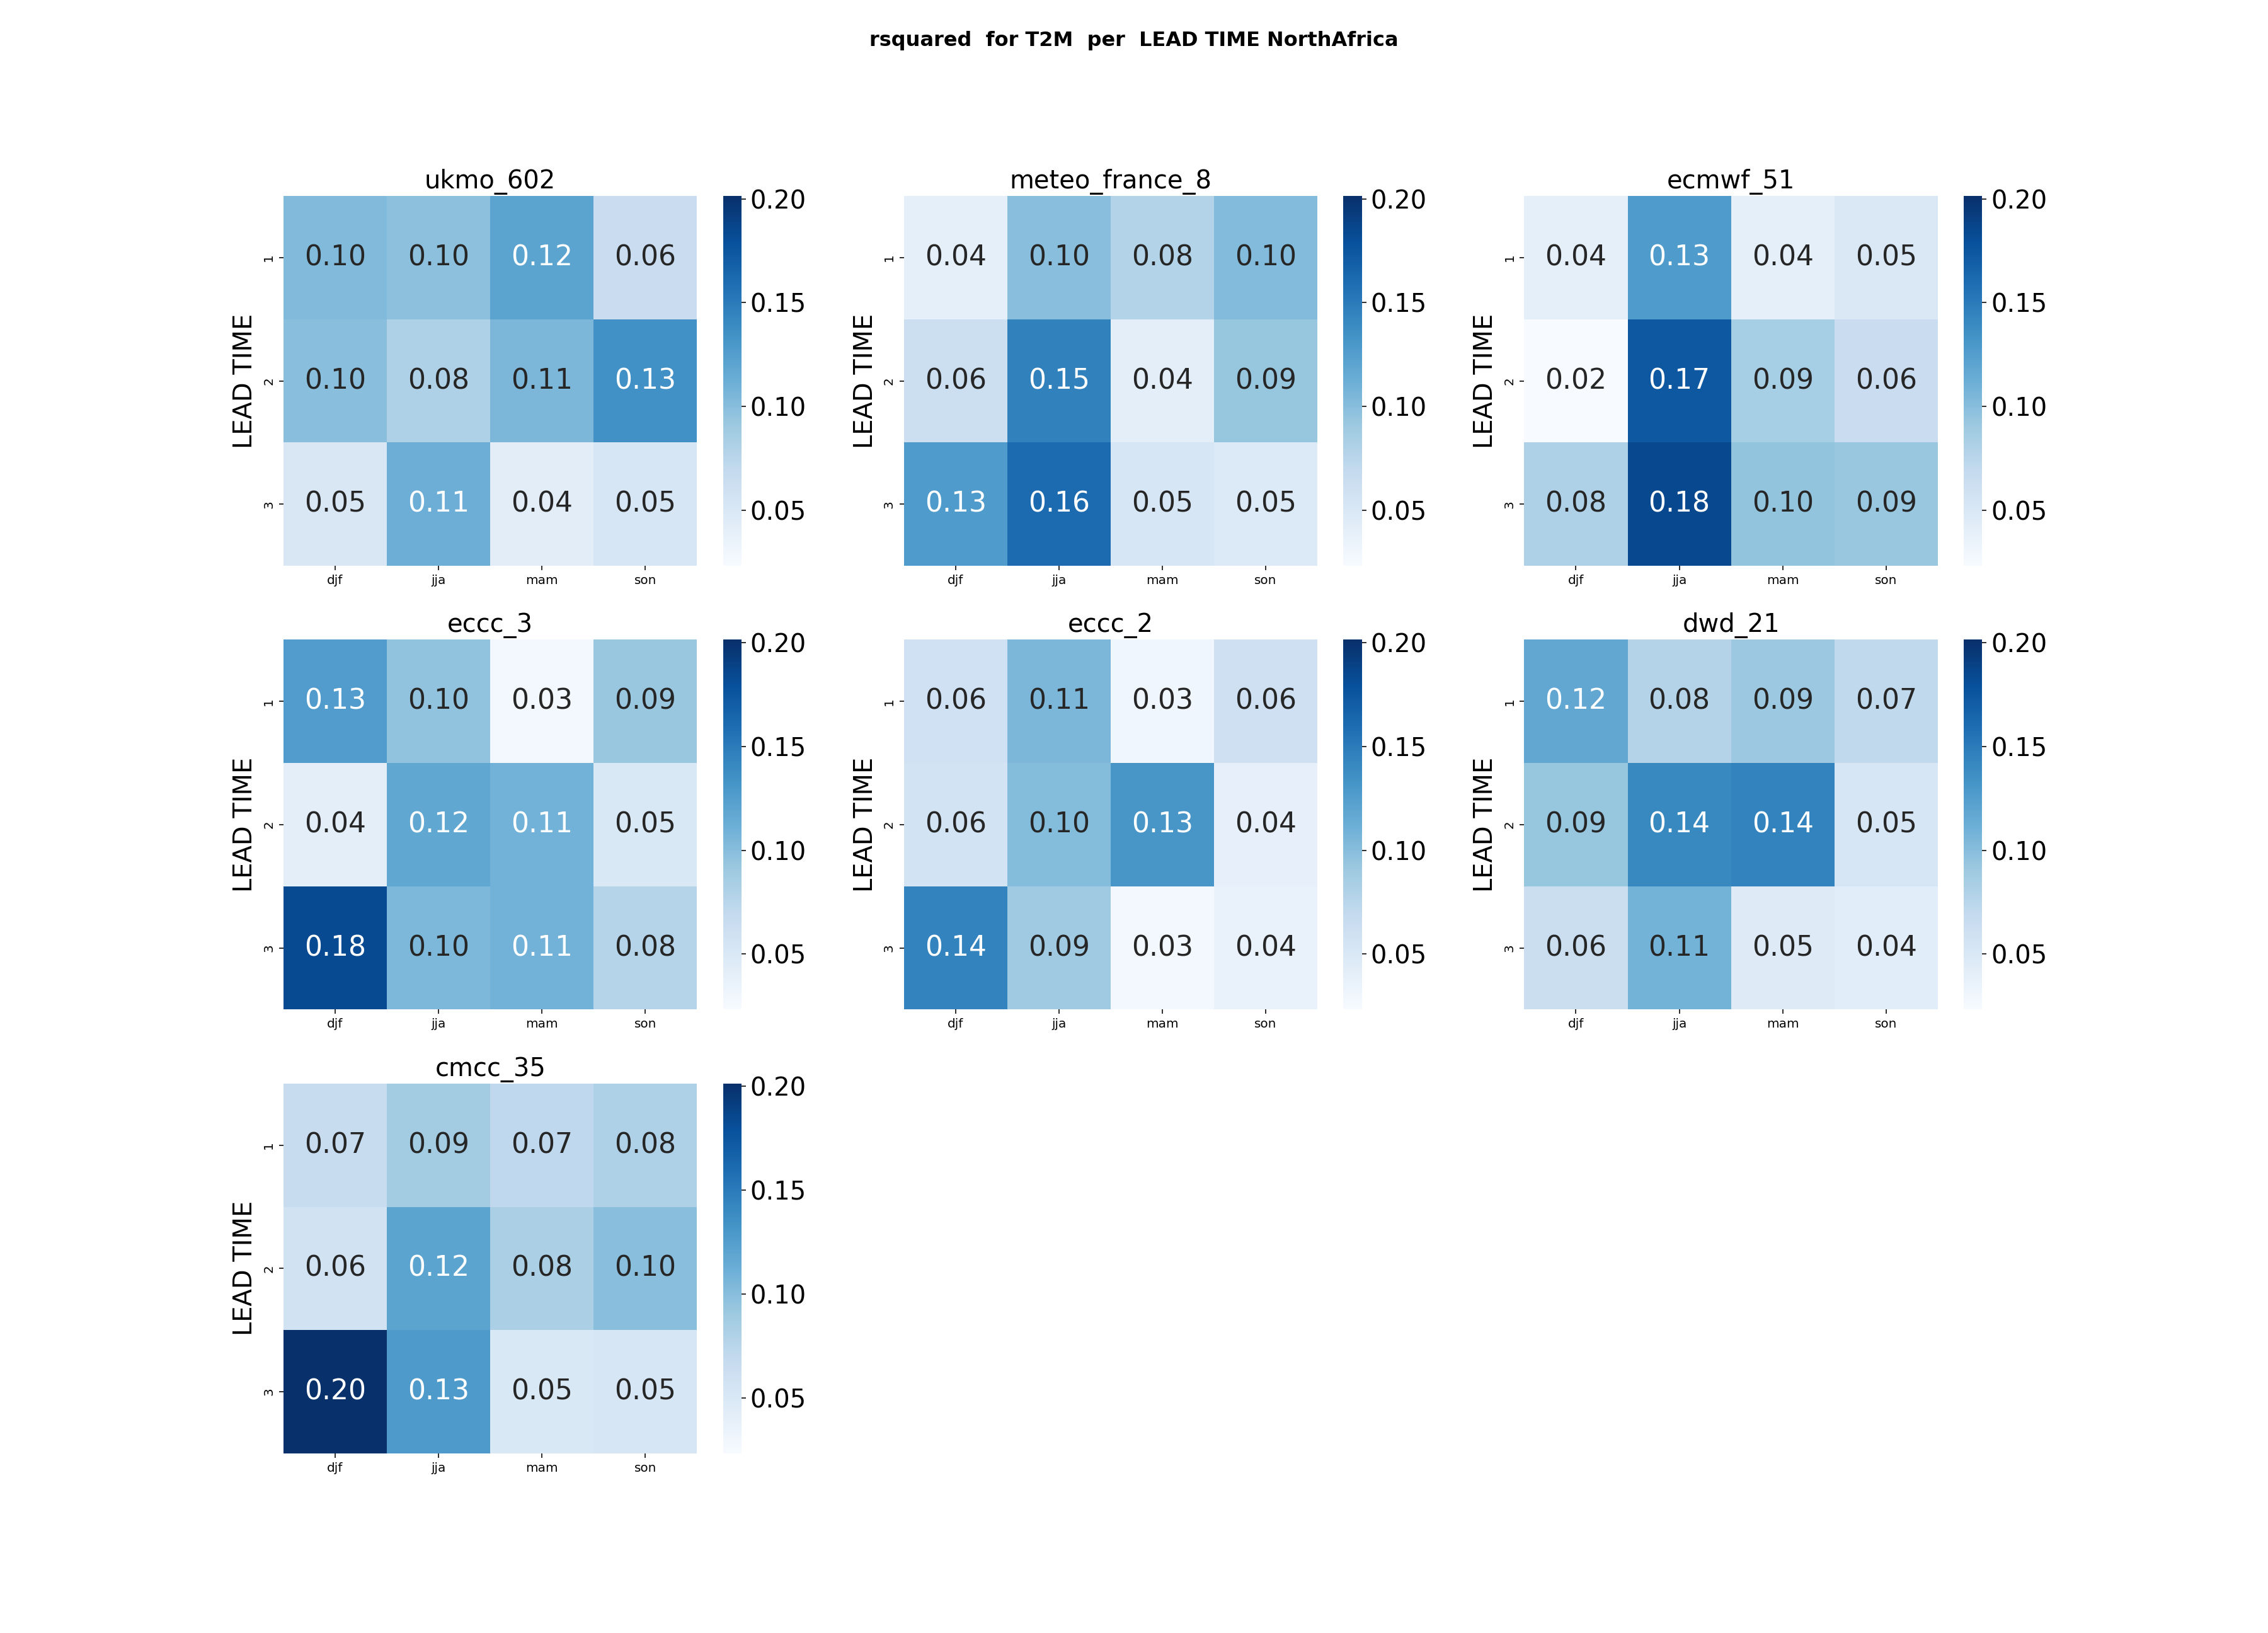
\includegraphics[width=1\linewidth]{plots/det/rsquared/rsquared_T2M_NorthAfrica.png}
    \caption{Temperature rsquared heatmaps for all the seasons}
\end{figure}
A closer look at North Africa reveals that the ECMWF model performs best during JJA, with R-SQUARED values increasing as the lead time increases-contrary to the trend observed for the MENA region as a whole, where performance typically decreases with longer lead times. This suggests that the ECMWF model is particularly adept at capturing the persistent summer temperature patterns in North Africa, which may benefit from stronger model predictability over time due to the relatively stable atmospheric and climatic conditions during JJA.

Similarly, Météo-France also shows good performance in North Africa, maintaining consistent R-SQUARED values across different lead times and seasons. This consistency highlights the model’s ability to handle the diverse climatic features of the region, such as the extreme temperatures influenced by the Sahara Desert and the moderating effects of the Mediterranean coastline.

These findings emphasize the importance of regional analysis, as the performance of climate models can vary significantly within sub-regions of MENA. While ECMWF excels in predicting North Africa’s summer temperatures, the observed increase in R-SQUARED with lead time underscores the need to investigate the underlying factors driving this unusual trend, which contrasts with the broader MENA region's dynamics.




\subsection{Probabilistic evaluation results}

To complement the deterministic evaluation of model performance, probabilistic evaluation metrics are employed to assess the reliability and skill of climate models in predicting the likelihood of specific outcomes. Unlike deterministic metrics, which focus on the accuracy of single-point predictions, probabilistic metrics evaluate the quality of the models’ forecast distributions, accounting for uncertainty and variability in predictions. These metrics are essential for understanding how well models represent the range of possible outcomes, particularly in regions like MENA, where climatic variability and extremes are prominent. By incorporating probabilistic metrics, this analysis provides a more comprehensive evaluation of the models’ predictive capabilities and their usefulness in decision-making under uncertainty.
The figures illustrate two main approaches to probabilistic assessment metrics, including the Brier Score (BS) and others. The first approach averages across lead times and grid points, while preserving categories, where the final figure contains the value of the metric for each season across all four seasons, for each category (mean, lower, upper) defined by the 1/3 quartiles. This method provides insight into the predictive ability of models under different seasonal conditions and forecast probability categories, particularly how well models capture temperature variations in the middle, lower, and upper quartiles of the predicted probability distribution. The diversity of metric values ​​across these categories helps highlight the sensitivity of models to different levels of forecast confidence. It indicates their ability to differentiate between forecast uncertainty and actual observed outcomes, providing a nuanced understanding of how accurately models predict different temperature ranges.

The second approach averages all grid points in the MENA region while retaining all lead times and seasons. This aggregated view provides an overall assessment of the measure for each season, considering all lead times and forecast categories. This approach focuses on how models perform across different forecast scenarios and how well they produce accurate and reliable temperature forecasts, regardless of forecast probability. By retaining lead times and seasons in the analysis, this method provides a comprehensive picture of model performance over time and under different climate conditions. It reveals how well models generalize across different forecast scenarios, helping to identify which models are most effective at producing consistent and reliable forecasts.
\subsubsection{Brier score}

The figure at the bottom illustrates that most models demonstrate relatively high performance, as indicated by a small Brier Score (BS), meaning that the predicted probabilities are close to the observed ones. This reflects accurate forecast probabilities forT2M The UKMO model, however, shows moderate performance with a larger BS, suggesting that its predicted probabilities are less closely aligned with observed outcomes compared to other models. Notably, the middle category presents lower performance relative to the other two categories (lower and upper). This indicates that while some models capture temperature variability well in extreme conditions (upper category), their skill diminishes when forecasting moderate changes (middle category). This discrepancy highlights the challenges models face in translating predicted probabilities into reliable forecasts, particularly for temperature variations that are neither extreme nor outlier events. 


\begin{figure}[H]
    \centering
    \includegraphics[width=1\linewidth]{plots/prob/bs/bs_T2M_category.png}
    \caption{Temperature Brier score heatmaps for all the seasons per categories}
\end{figure}
An analysis by lead time revealed that the models Meteo France, ECMWF, and CMCC exhibit superior performance, as indicated by lower Brier Scores (BS). This suggests that these models provide more accurate probabilistic forecasts for T2M compared to others. Moreover, the differences in BS values between successive lead times are minimal, indicating that the predictive skill of these models remains relatively consistent as the forecast horizon increases.

This stability in performance across lead times is particularly noteworthy, as it reflects the robustness of these models in maintaining their ability to produce reliable forecasts over time. The lower BS values also suggest that these models effectively capture the relationship between predicted probabilities and observed outcomes, ensuring high confidence in their probabilistic predictions. Such consistent performance across lead times is crucial for operational forecasting, as it highlights these models' reliability for both short- and medium-term forecasts in the MENA region.

\begin{figure}[H]
    \centering
    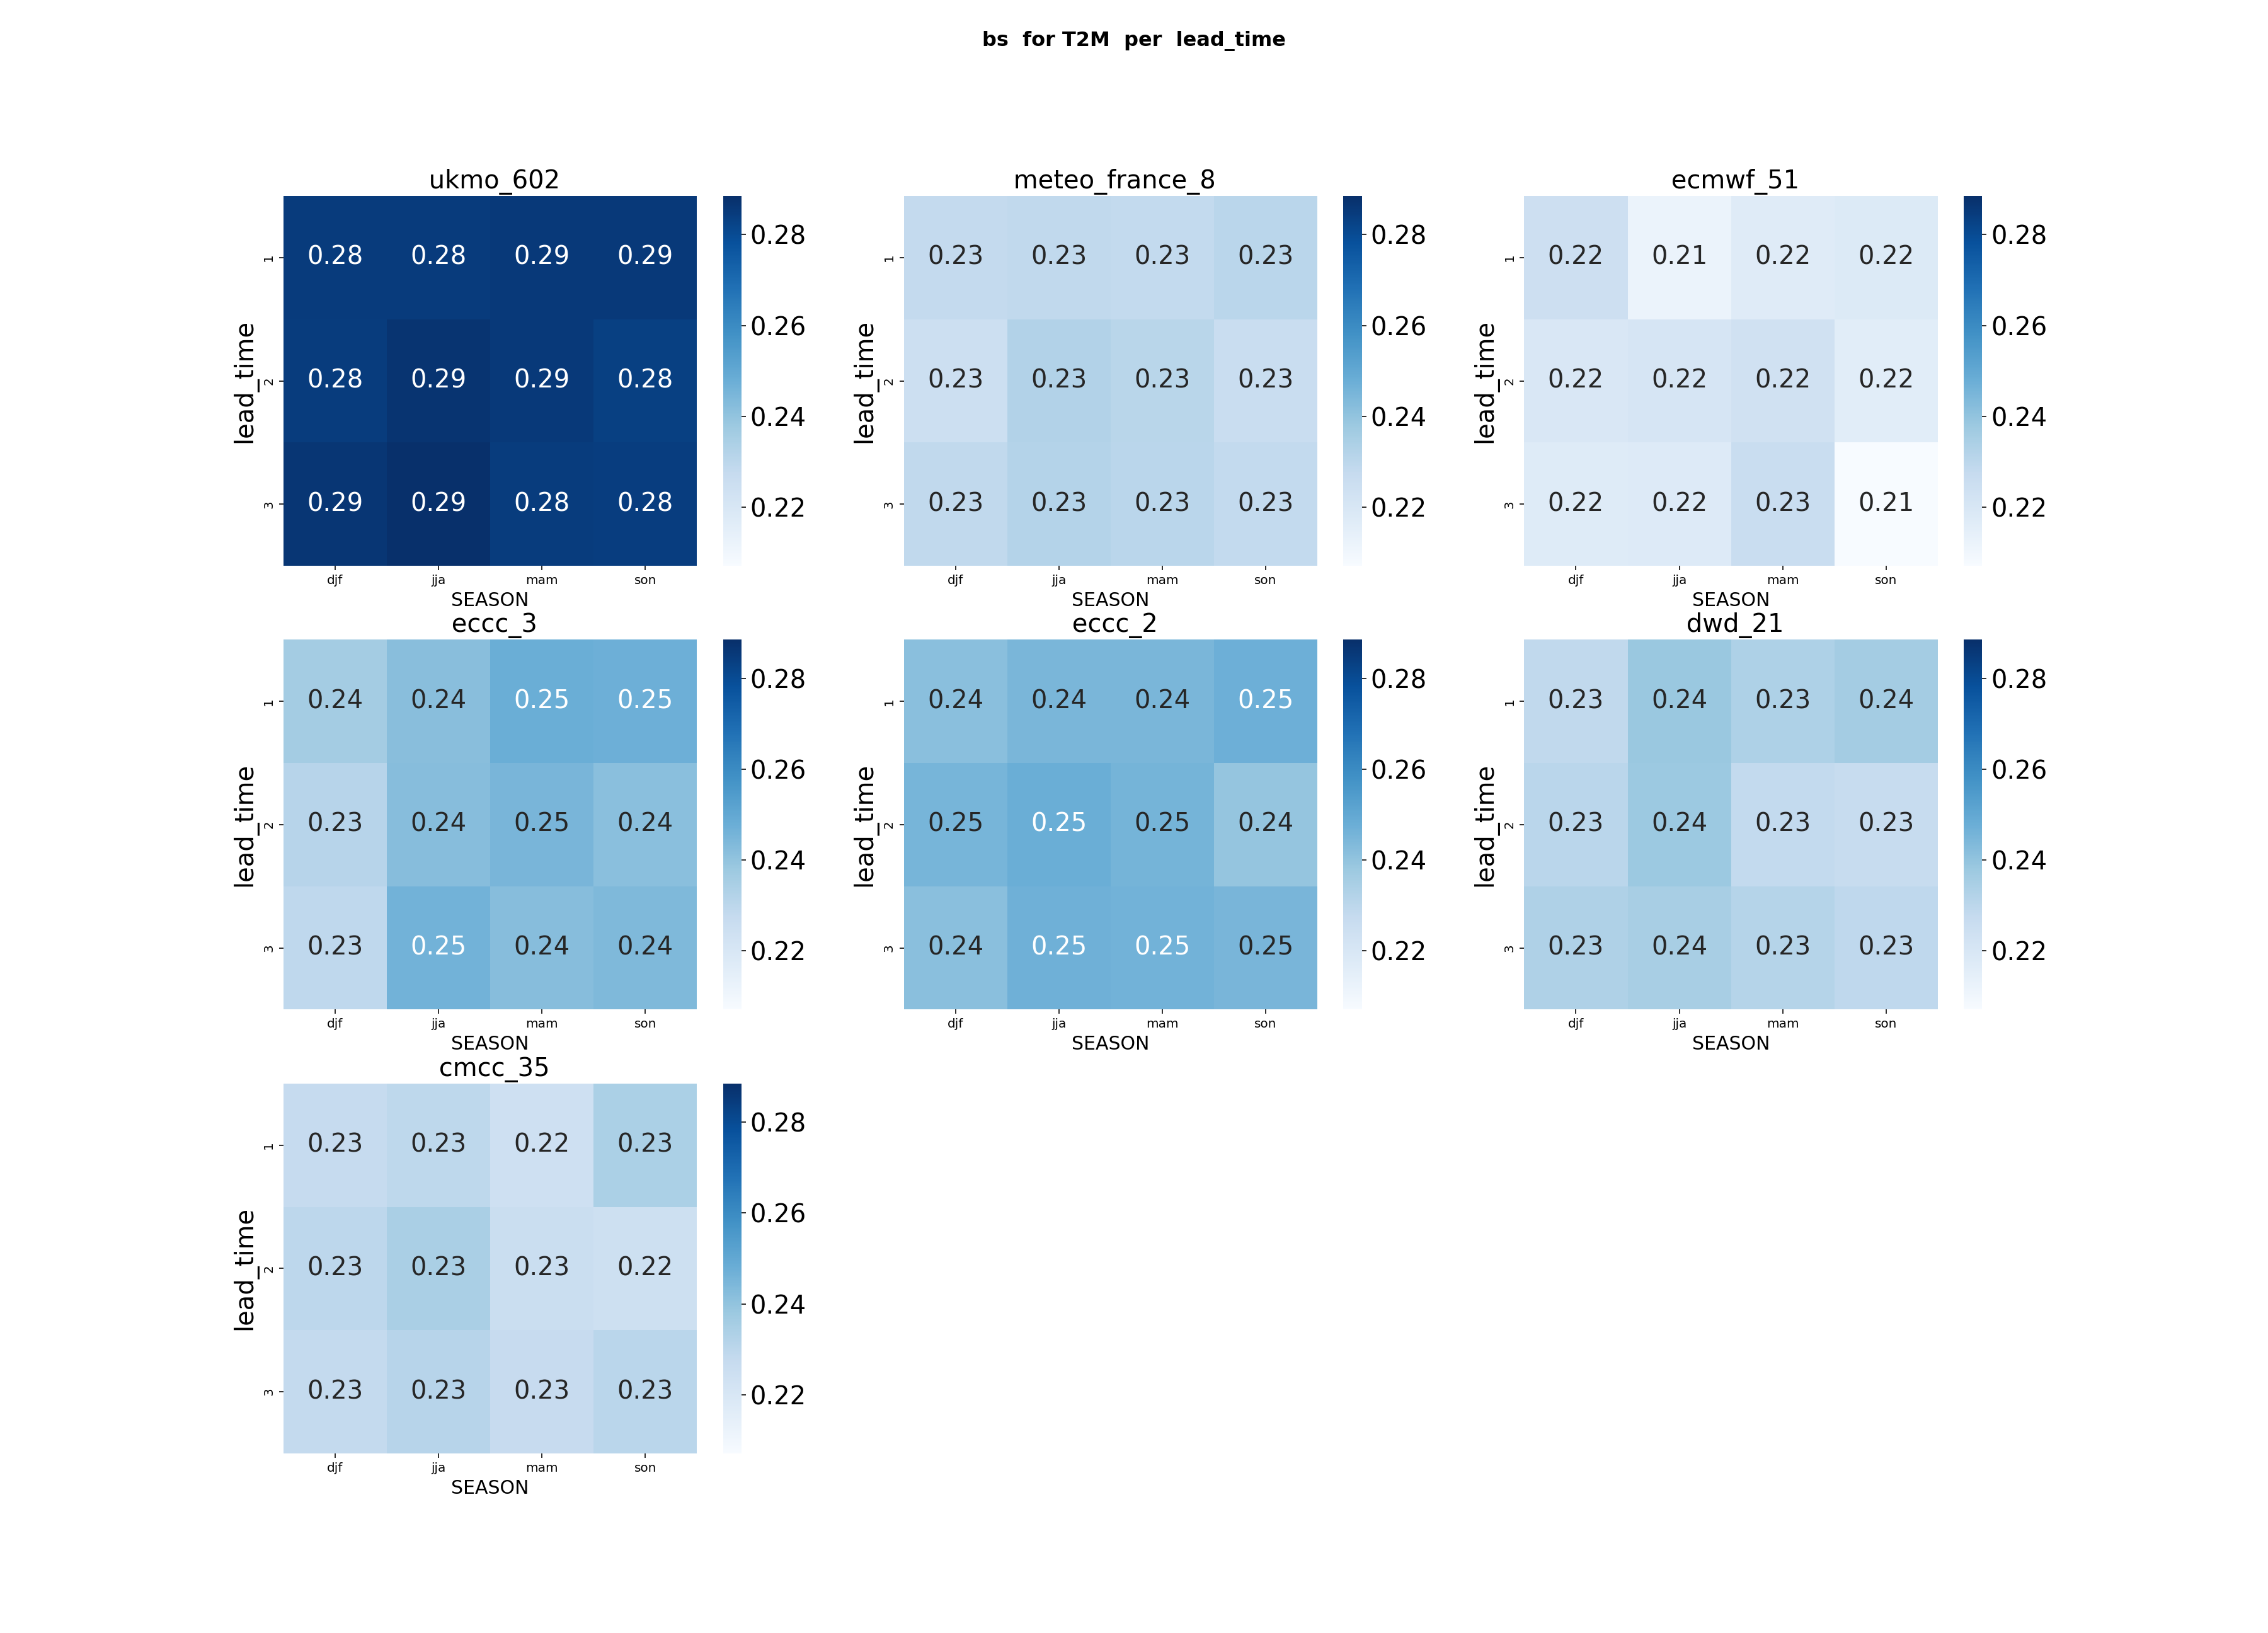
\includegraphics[width=1\linewidth]{plots/prob/bs/bs_T2M_lead_time.png}
    \caption{Temperature brier score heatmaps for all the seasons per lead time}
\end{figure}
o further evaluate the performance of these models and assess whether the same interpretations apply, the analysis will now focus specifically on the North African region. By examining the Brier Score metrics in this sub-region, we aim to determine whether the observed trends, such as the consistency of model performance across lead times and the relative strengths of ECMWF, CMCC, and Meteo France, remain valid or if different patterns emerge due to the unique climatic conditions and variability in North Africa.

\begin{figure}[H]
    \centering
    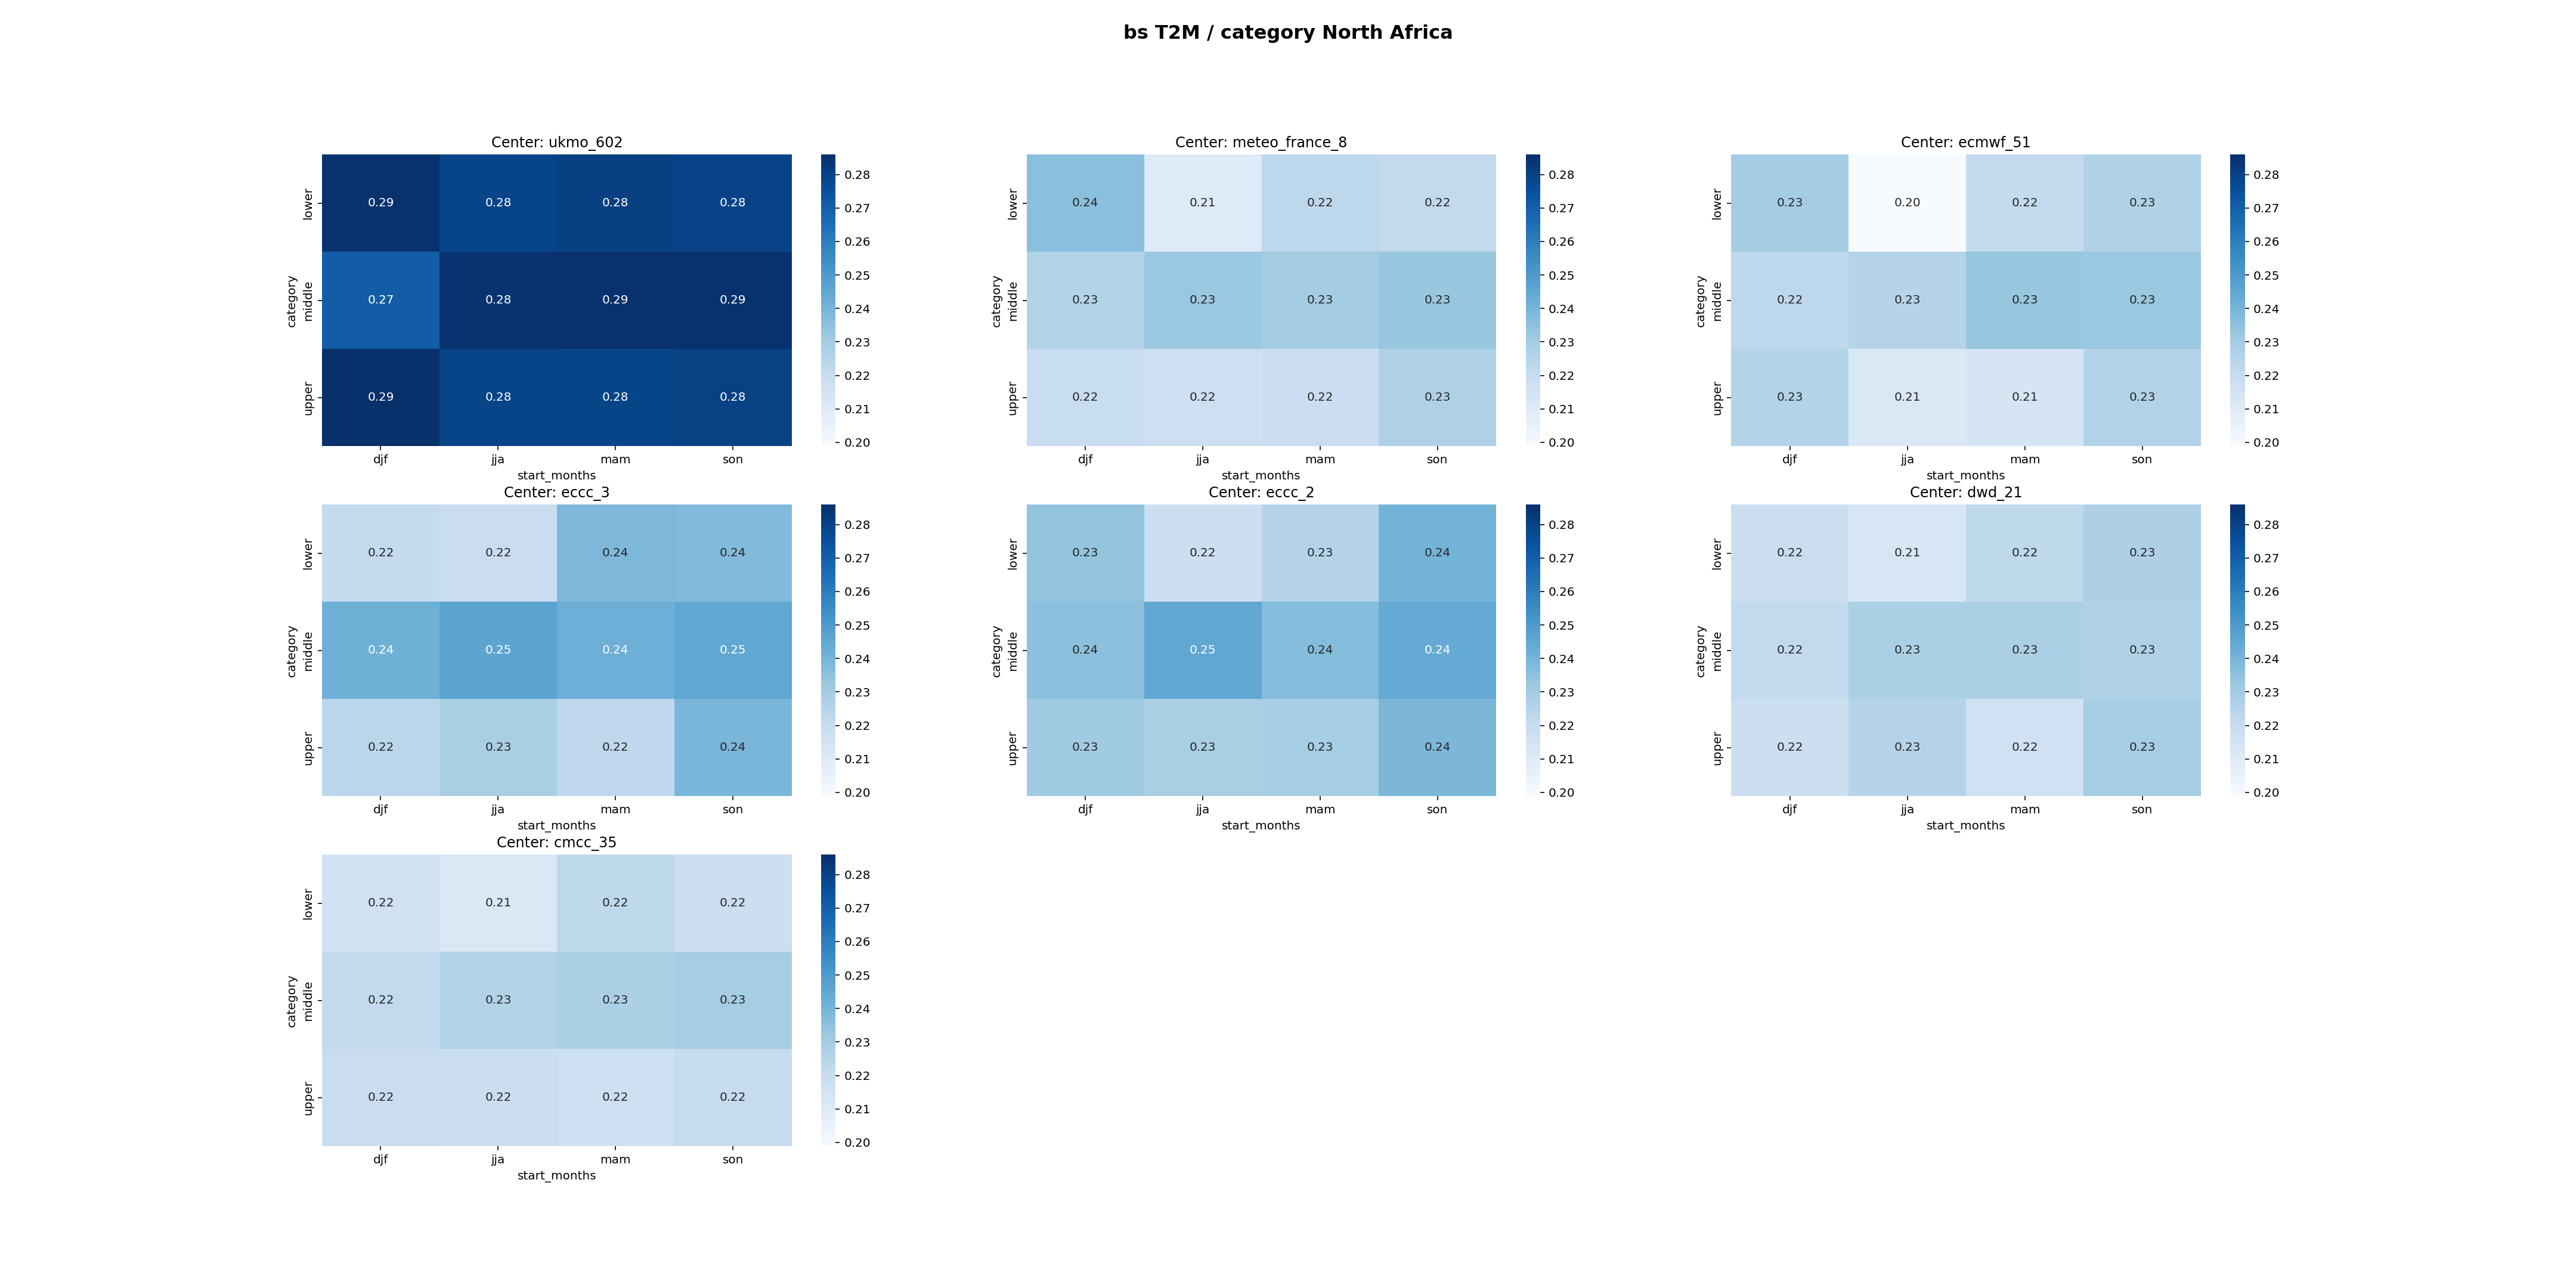
\includegraphics[width=1\linewidth]{plots/prob/bs/bs_T2M_category_North_Africa.png}
    \caption{Temperature Brier score heatmaps for all the seasons per categories for north africa}
\end{figure}
A closer analysis focused on the North African region revealed that the performance of the top-performing models—ECMWF, CMCC, and Meteo France—remains consistent. The zoomed evaluation shows that these models continue to exhibit low Brier Scores, indicating reliable probabilistic predictions across lead times. This finding suggests that the unique climatic conditions of North Africa do not significantly alter the predictive skill of these models, reaffirming their robustness and adaptability to sub-regional variations within the broader MENA context.


\begin{figure}[H]
    \centering
    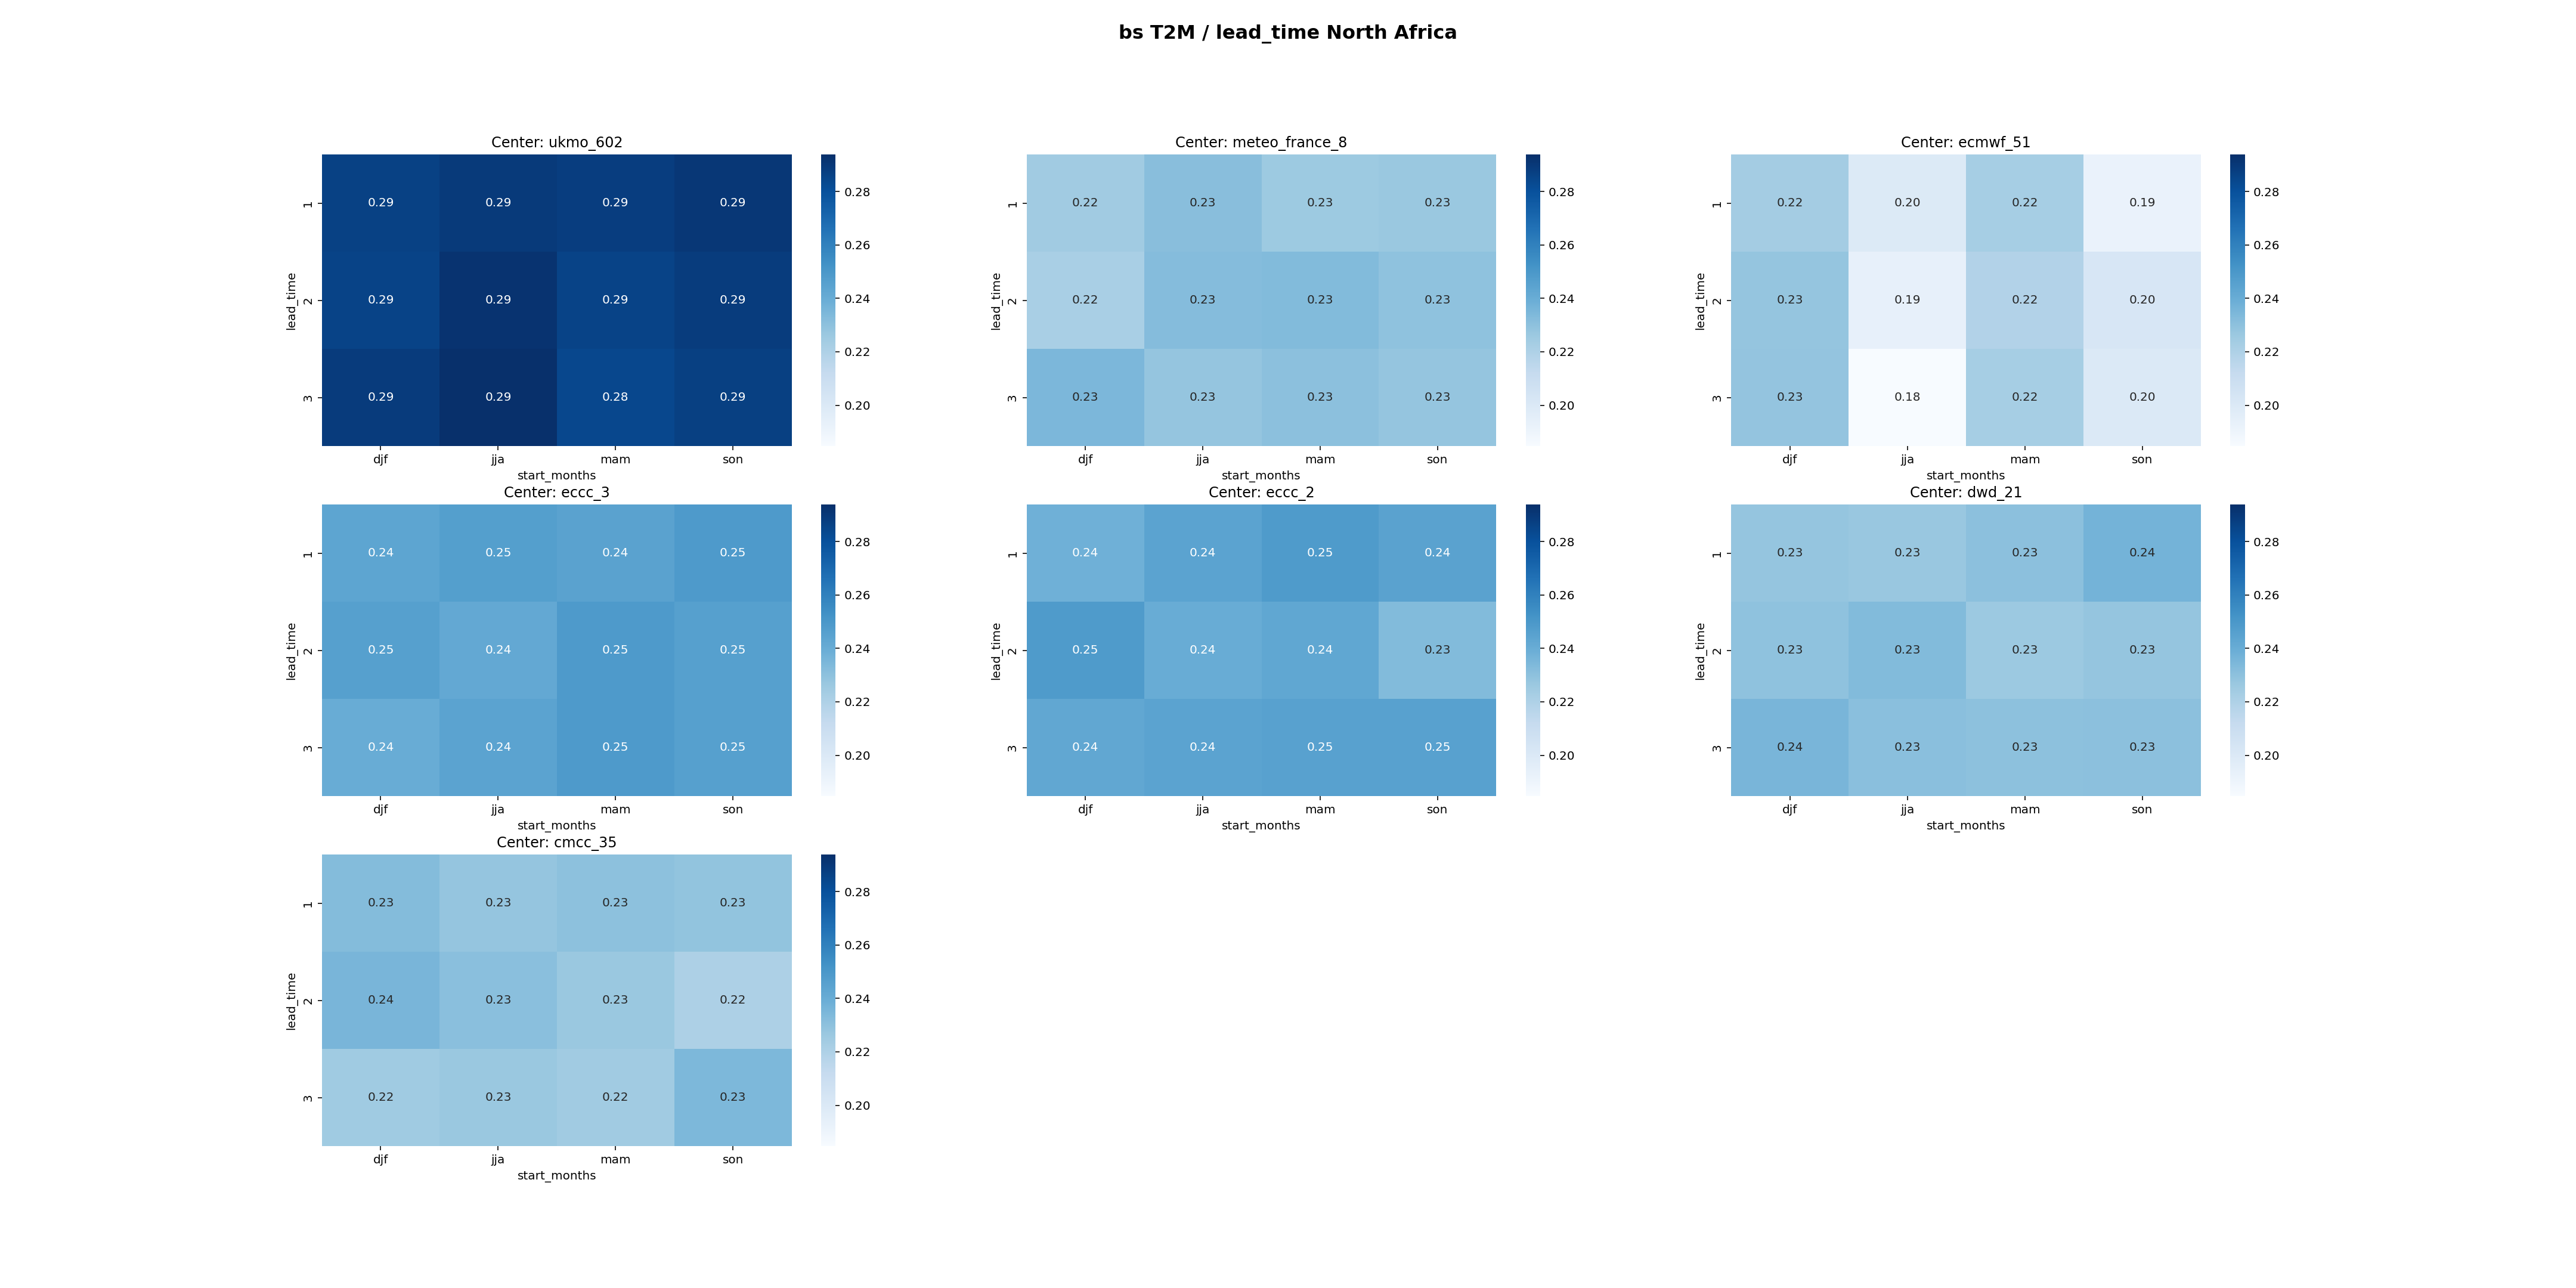
\includegraphics[width=1\linewidth]{plots/prob/bs/bs_T2M_lead_time_North_Africa.png}
    \caption{Temperature brier score heatmaps for all the seasons per lead time}
\end{figure}
The results by lead time reveal similar conclusions, showing a consistent stability in Brier Scores across different lead times. This indicates that the predictive skill of the top-performing models, such as ECMWF, CMCC, and Meteo France, remains robust even as the forecast horizon increases. The minimal variation in scores across lead times underscores the reliability of these models for producing accurate probabilistic forecasts, regardless of the temporal range considered.
\subsubsection{Reliability}
The reliability diagrams presented for the season assess the probabilistic performance of the seven climate models across three forecast categories: lower tercile , middle tercile , and upper tercile . These diagrams compare the predicted forecast probabilities to the observed frequencies, providing a clear indication of the models' ability to produce reliable temperature forecasts. A perfectly reliable model would align closely with the diagonal, where predicted probabilities match observed outcomes. By analyzing these diagrams, we can identify which models perform best for specific categories and uncover any systematic biases, such as over- or under-forecasting certain probabilities. This evaluation is crucial for understanding the strengths and weaknesses of the models, particularly in their ability to capture temperature extremes and moderate conditions .


\begin{figure}[H]
    \centering
    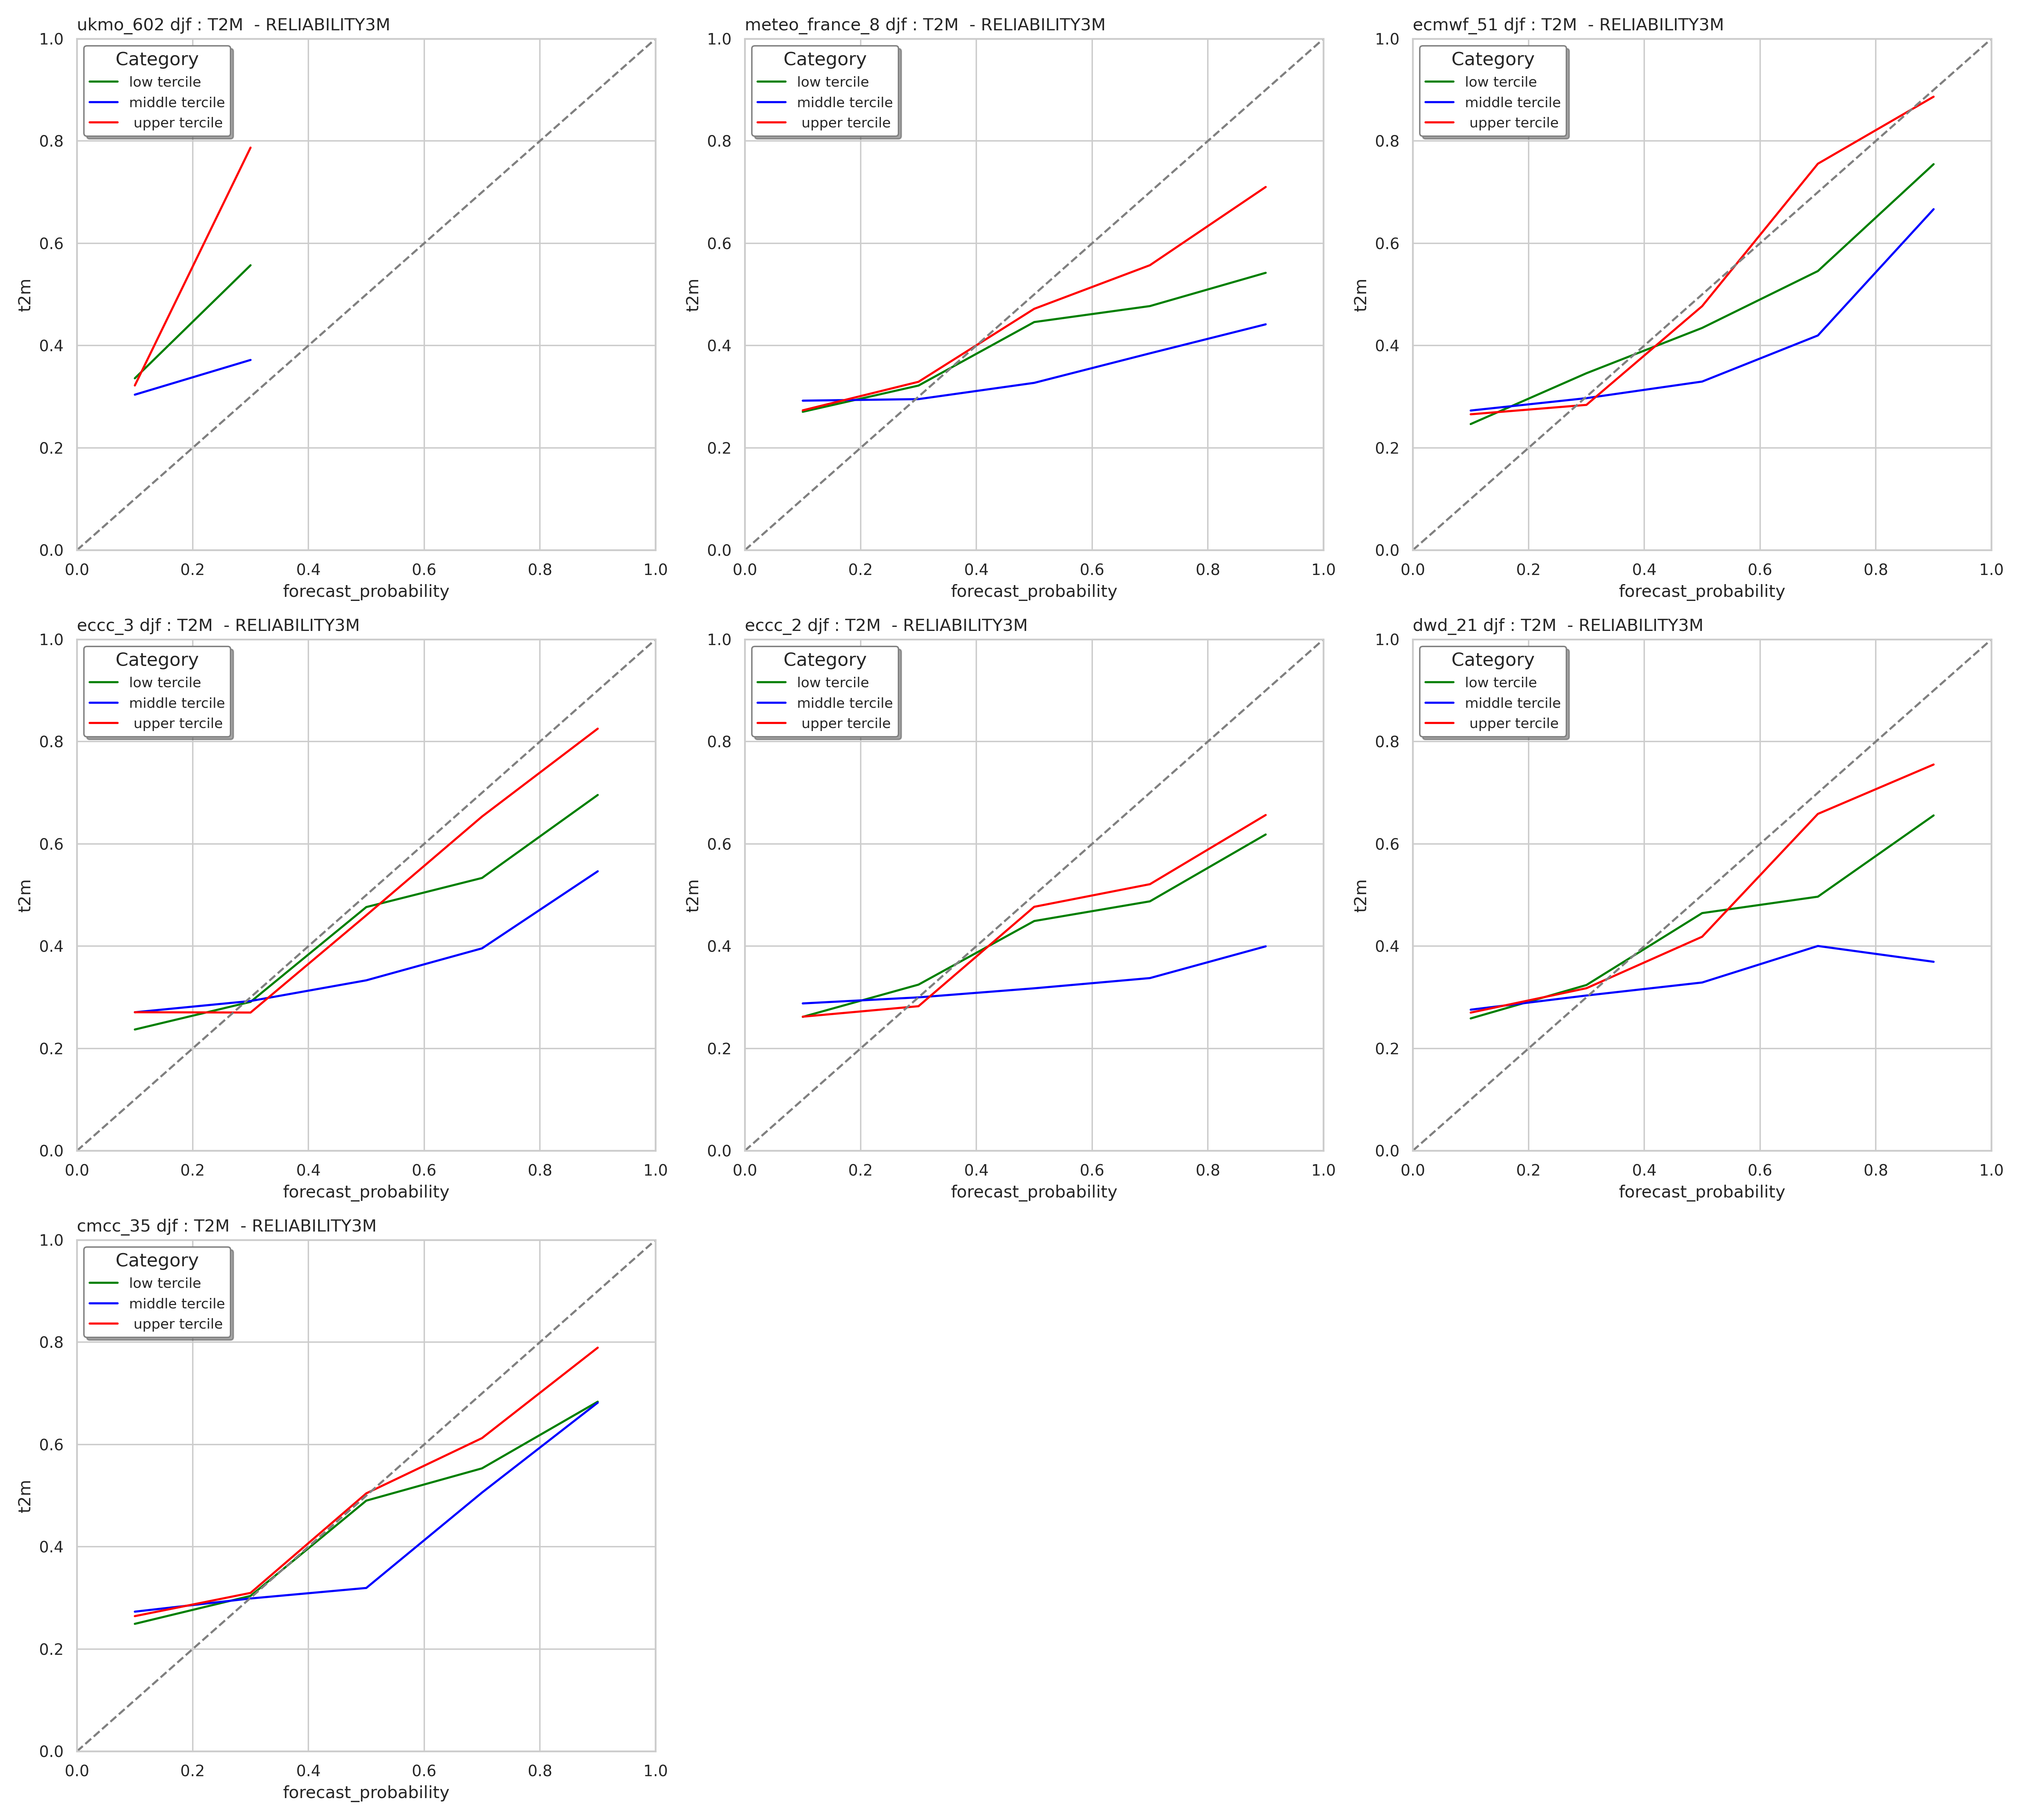
\includegraphics[width=1\linewidth]{plots/prob/rela/rela_diagram_t2m_djf.png}
    \caption{temperature reliabilty maps for djf}
\end{figure}

For the DJF season, the reliability diagrams show that most models exhibit similar performance, with the exception of UKMO, which significantly overestimates probabilities across all categories. For ECMWF, there is a noticeable overestimation in the upper tercile (warm extremes) starting at a forecast probability of approximately 0.6, indicating that the model tends to assign higher probabilities to warm events compared to their observed frequencies. Conversely, ECMWF shows a systematic underestimation for both the lower and middle terciles across most probabilities. For the remaining models, except UKMO, there is a general trend of underestimation across all three categories, beginning at forecast probabilities around 0.5. This pattern suggests that while the models capture some aspects of the observed temperature distribution, they struggle to provide accurate probabilities for more extreme or moderate conditions, especially at higher forecast probabilities. These results highlight the challenges faced by the models in reliably predicting temperature outcomes during the winter season (DJF), particularly for extreme categories.
For the other three seasons (JJA, MAM, and SON), the reliability diagrams reveal a general tendency for most models to underestimate probabilities across all tercile categories, starting at approximately 0.4. This underestimation indicates that the models tend to be over-cautious, predicting lower probabilities than what is observed in reality. However, UKMO still stands out as an exception, showing a consistent overestimation across the forecast range, particularly for higher probabilities. This suggests that UKMO tends to assign excessively high probabilities to events that occur less frequently than predicted, which reduces its reliability. Overall, this recurring underestimation in the majority of models highlights their difficulty in accurately capturing the likelihood of temperature outcomes, especially beyond moderate probabilities. 

\begin{figure}[H]
    \centering
    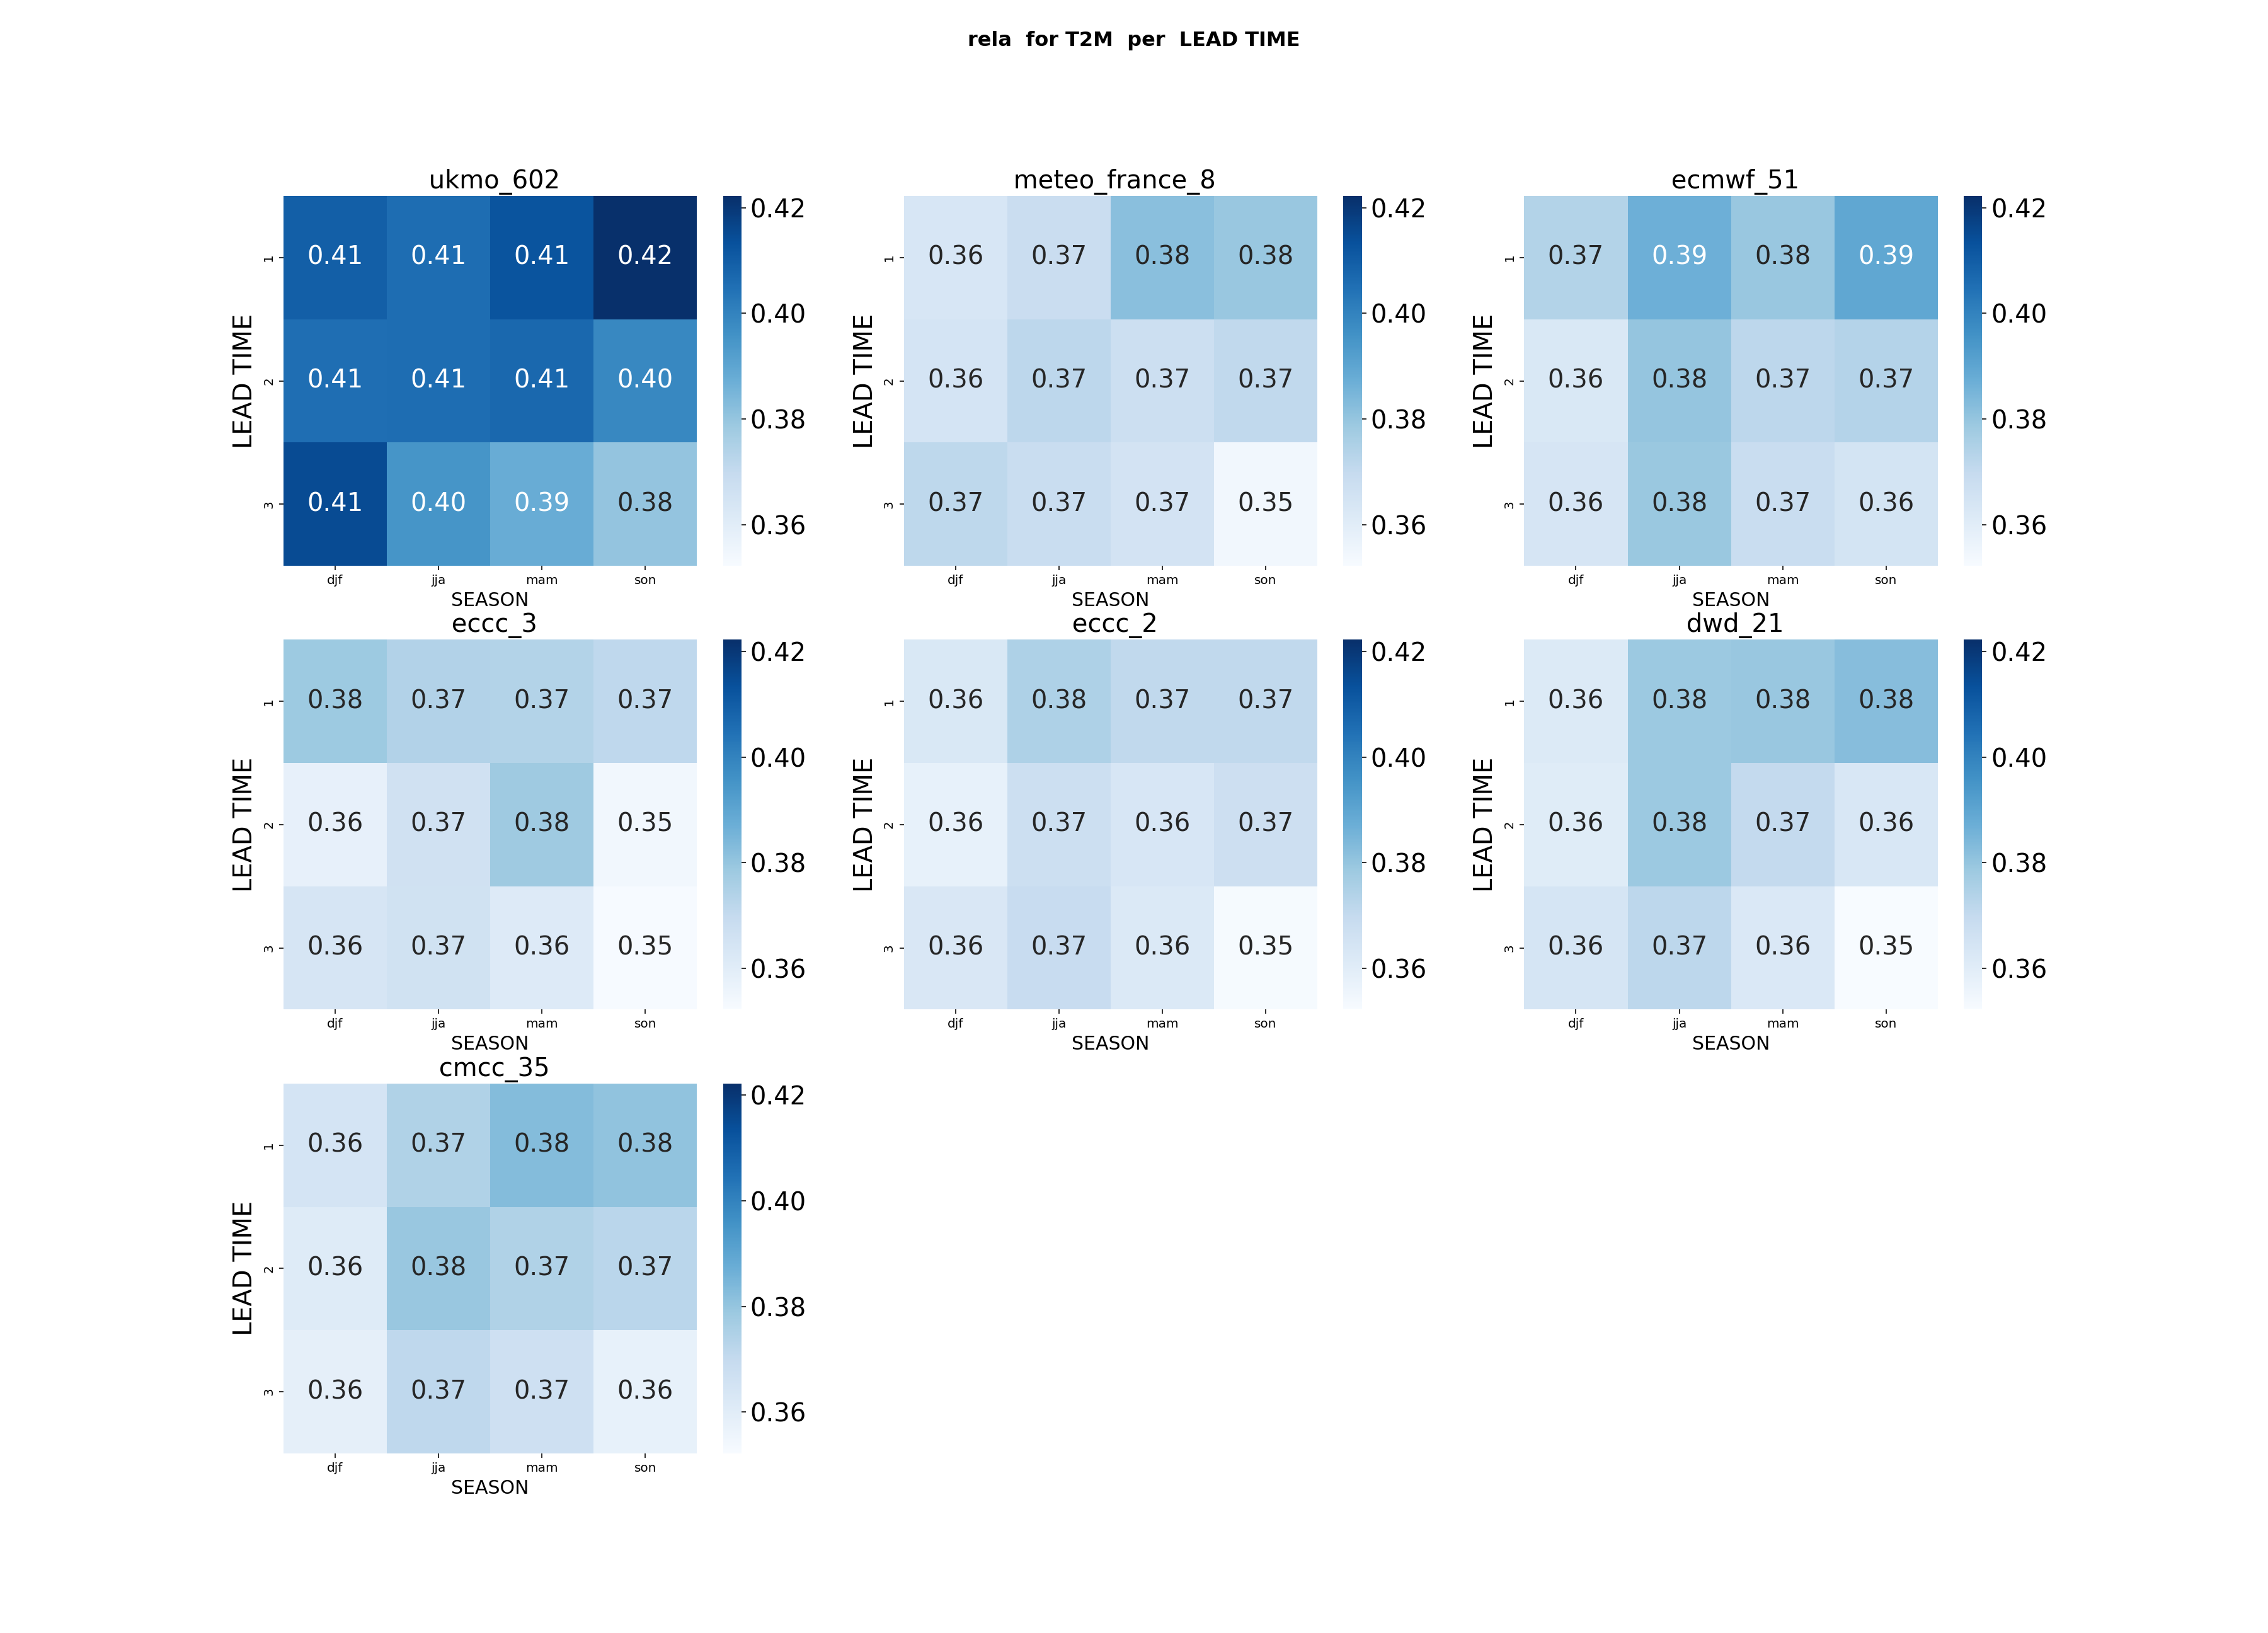
\includegraphics[width=1\linewidth]{plots/prob/rela/rela_T2M.png}
    \caption{temperature reliabilty heatmap}
\end{figure}
The heatmap further confirms the analyses derived from the reliability diagrams. It highlights similar trends observed across the models and seasons.Conversely, UKMO continues to stand out with its consistent overestimation of probabilities, aligning with the overconfidence seen in the reliability diagrams. This agreement between the heatmap and the reliability curves strengthens confidence in the identified patterns .
\begin{figure}[H]
    \centering
    \includegraphics[width=1\linewidth]{plots/prob/rela/rela_T2M_NorthAfrica.png}
    \caption{temperature reliabilty heatmap for north africa}
\end{figure}

A more focused analysis on North Africa has not significantly altered the overall conclusions derived from the broader MENA region. The consistent performance patterns observed across the different models and seasons remain largely unchanged when examining the North African context. 




\subsubsection{The ranked probability score }

The Ranked Probability Score (RPS) provides a valuable measure of forecast performance by evaluating the accuracy of probabilistic predictions across different categories. It combines both the skill in predicting the occurrence of events and the sharpness of the forecast distribution. By comparing the forecasted probability distribution against the observed outcomes, the RPS quantifies the deviation between the predicted and actual probabilities. A lower RPS value indicates better forecast accuracy, reflecting both how well the forecast aligns with observed frequencies and how well it discriminates between different probability categories. This metric helps to identify which models offer the most reliable probabilistic predictions, particularly in terms of capturing the likelihood of various temperature outcomes within a given forecast period.
\begin{figure}[H]
    \centering
    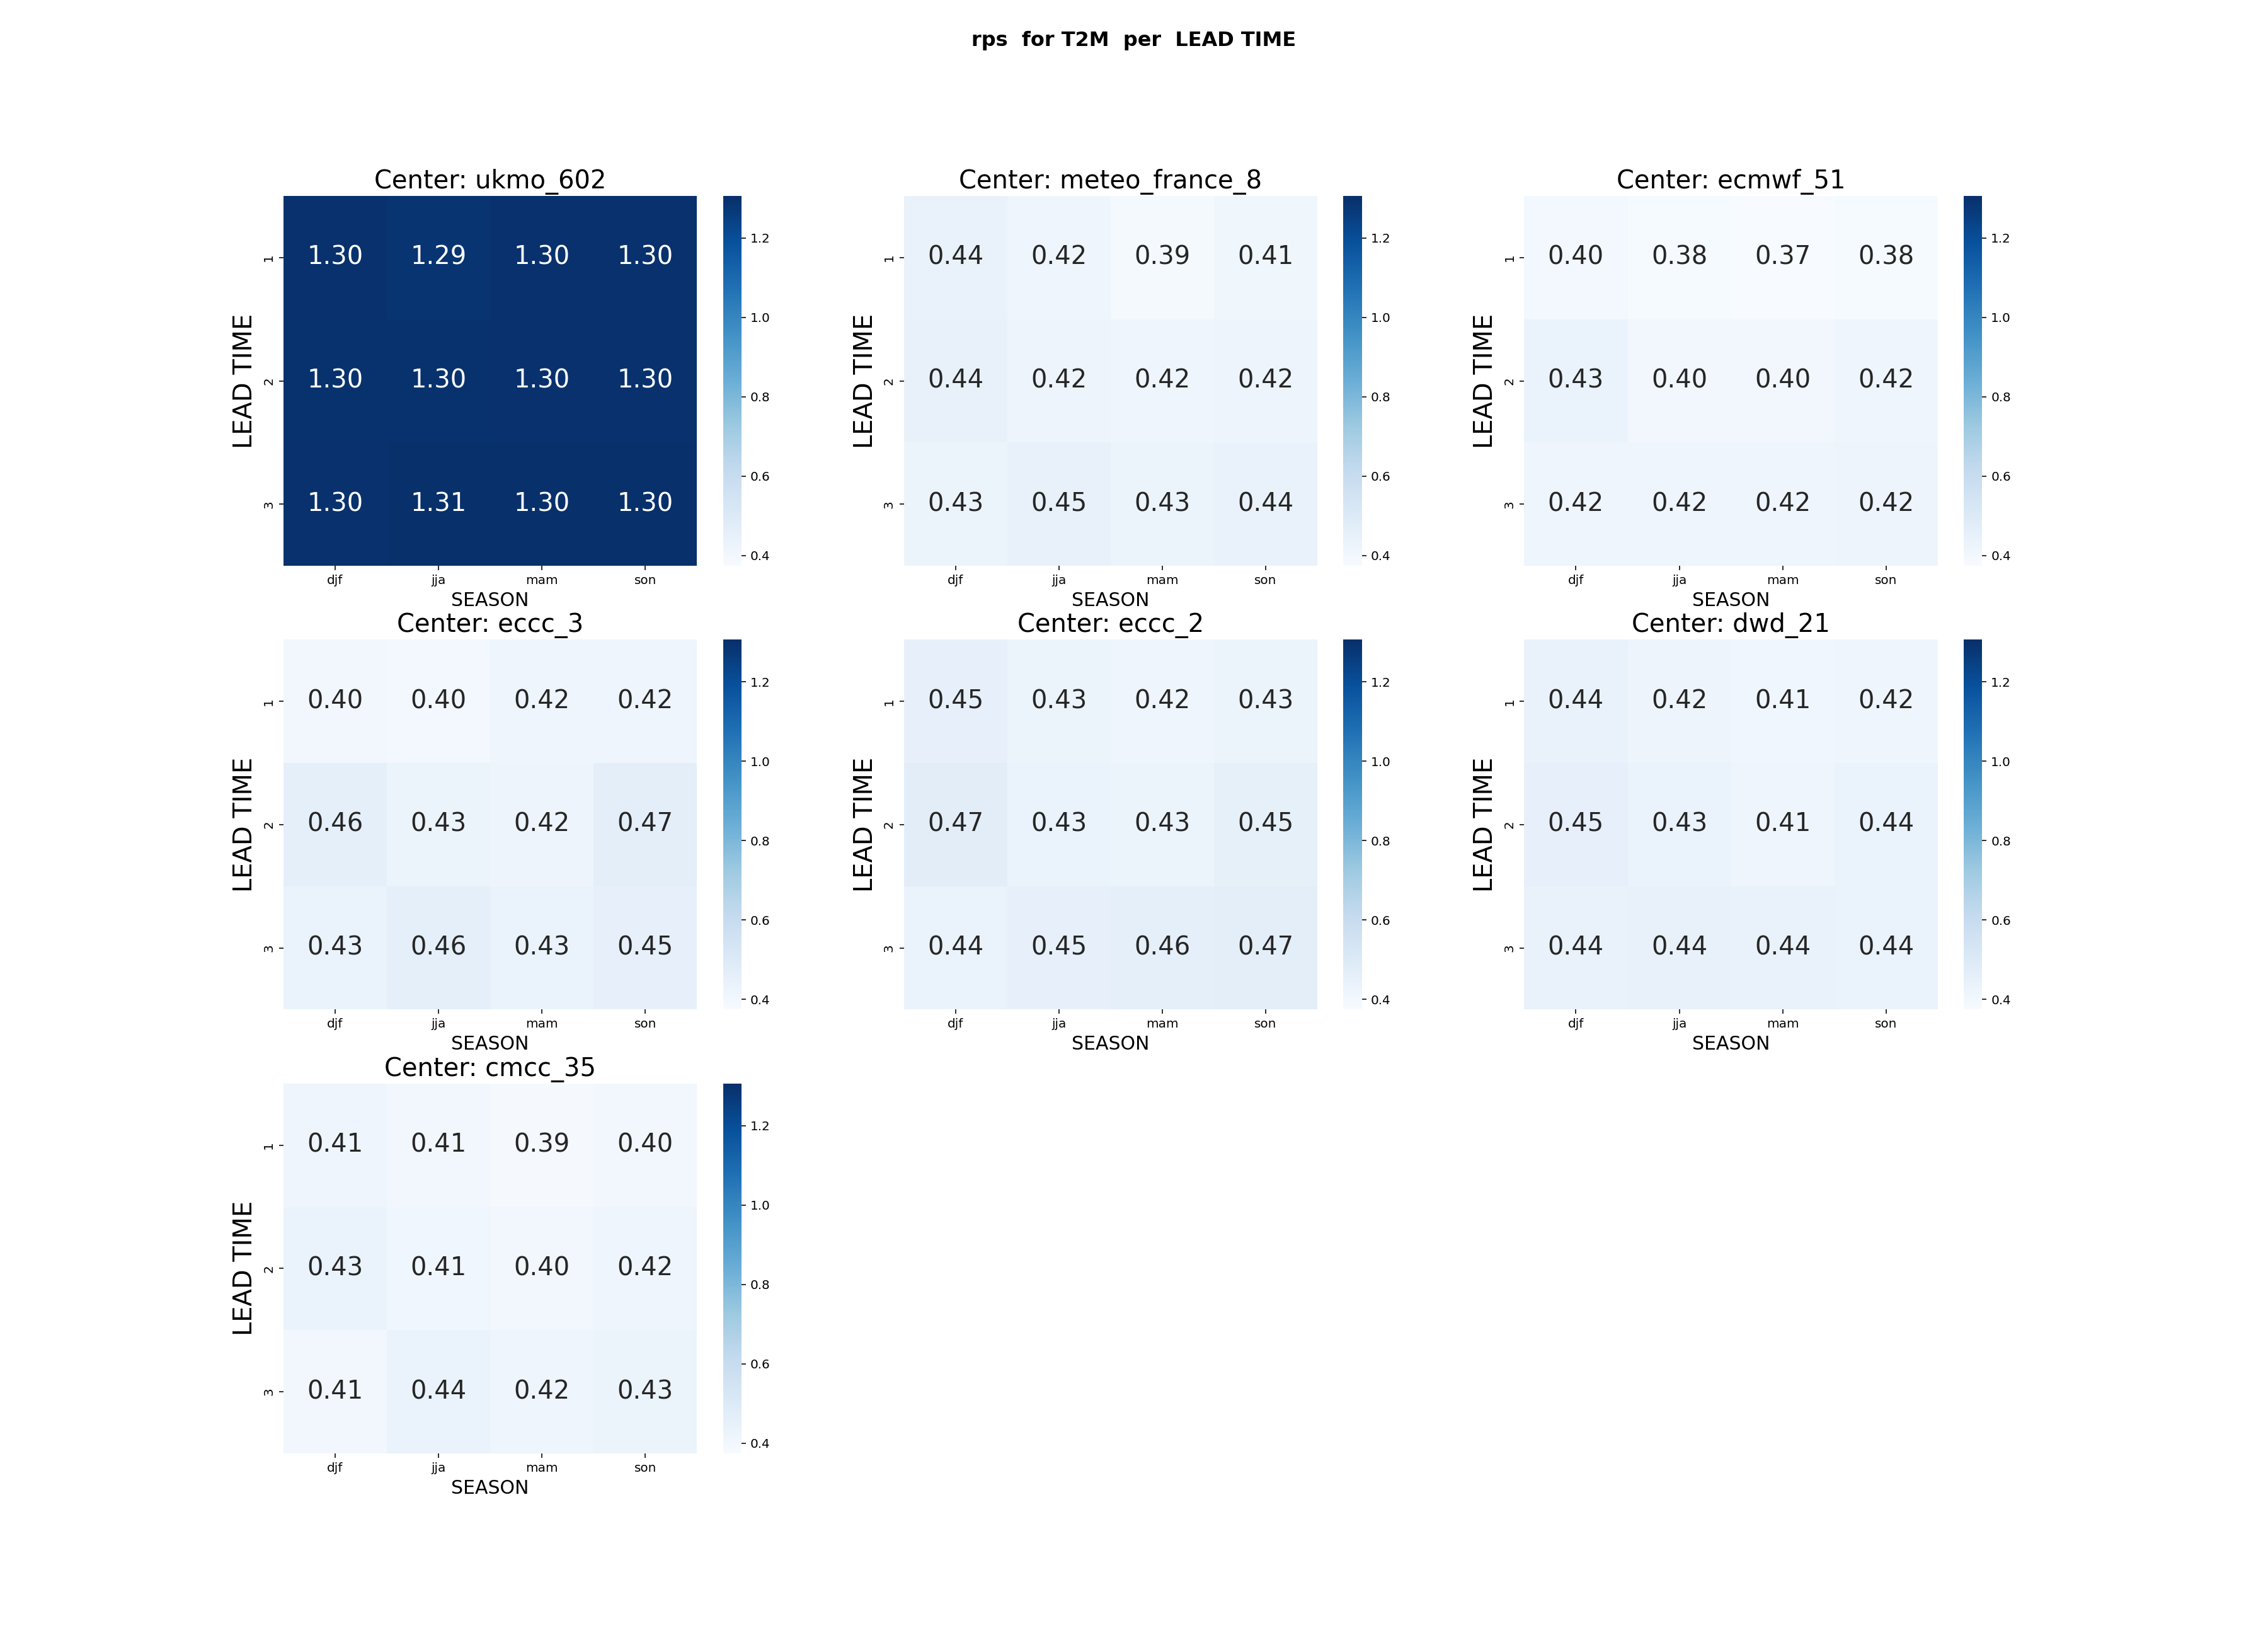
\includegraphics[width=1\linewidth]{plots/prob/rps/rps_T2M.png}
    \caption{Temperature RPS  heatmaps for all the seasons per categories}
\end{figure}
The figure displaying the Ranked Probability Score (RPS) for different climate models and seasonal periods provides a detailed view of model performance across various start months (DJF, JJA, MAM, SON). Each cell in the matrix represents the RPS value for a specific model and season combination, with the color intensity indicating how well the forecast probabilities match the observed data.

From this figure, it is evident that ECMWF consistently shows lower RPS values, indicating better predictive accuracy across different seasons. This suggests that ECMWF's forecasts are more closely aligned with observed temperature variability. The relatively higher RPS values for  UKMO model underscore their challenges in accurately capturing temperature variations. 
For the North African region, the results mirror those observed in the broader MENA region.  

This suggests that despite the localized focus on North Africa, the model performance differences remain significant, particularly for UKMO. 



\begin{figure}[H]
    \centering
    \includegraphics[width=1\linewidth]{plots/prob/rps/rps_T2M_NorthAfrica.png}
    \caption{Temperature RPS  heatmaps for north africa}
\end{figure}
\subsubsection{Receiver Operating Characteristic}
The ROC (Receiver Operating Characteristic) curve is an important tool for evaluating the performance of predictive models, particularly in the context of probabilistic forecasts. It provides a graphical representation of the trade-off between the true positive rate  and the false positive rate  across various threshold levels.

\begin{figure}[H]
    \centering
    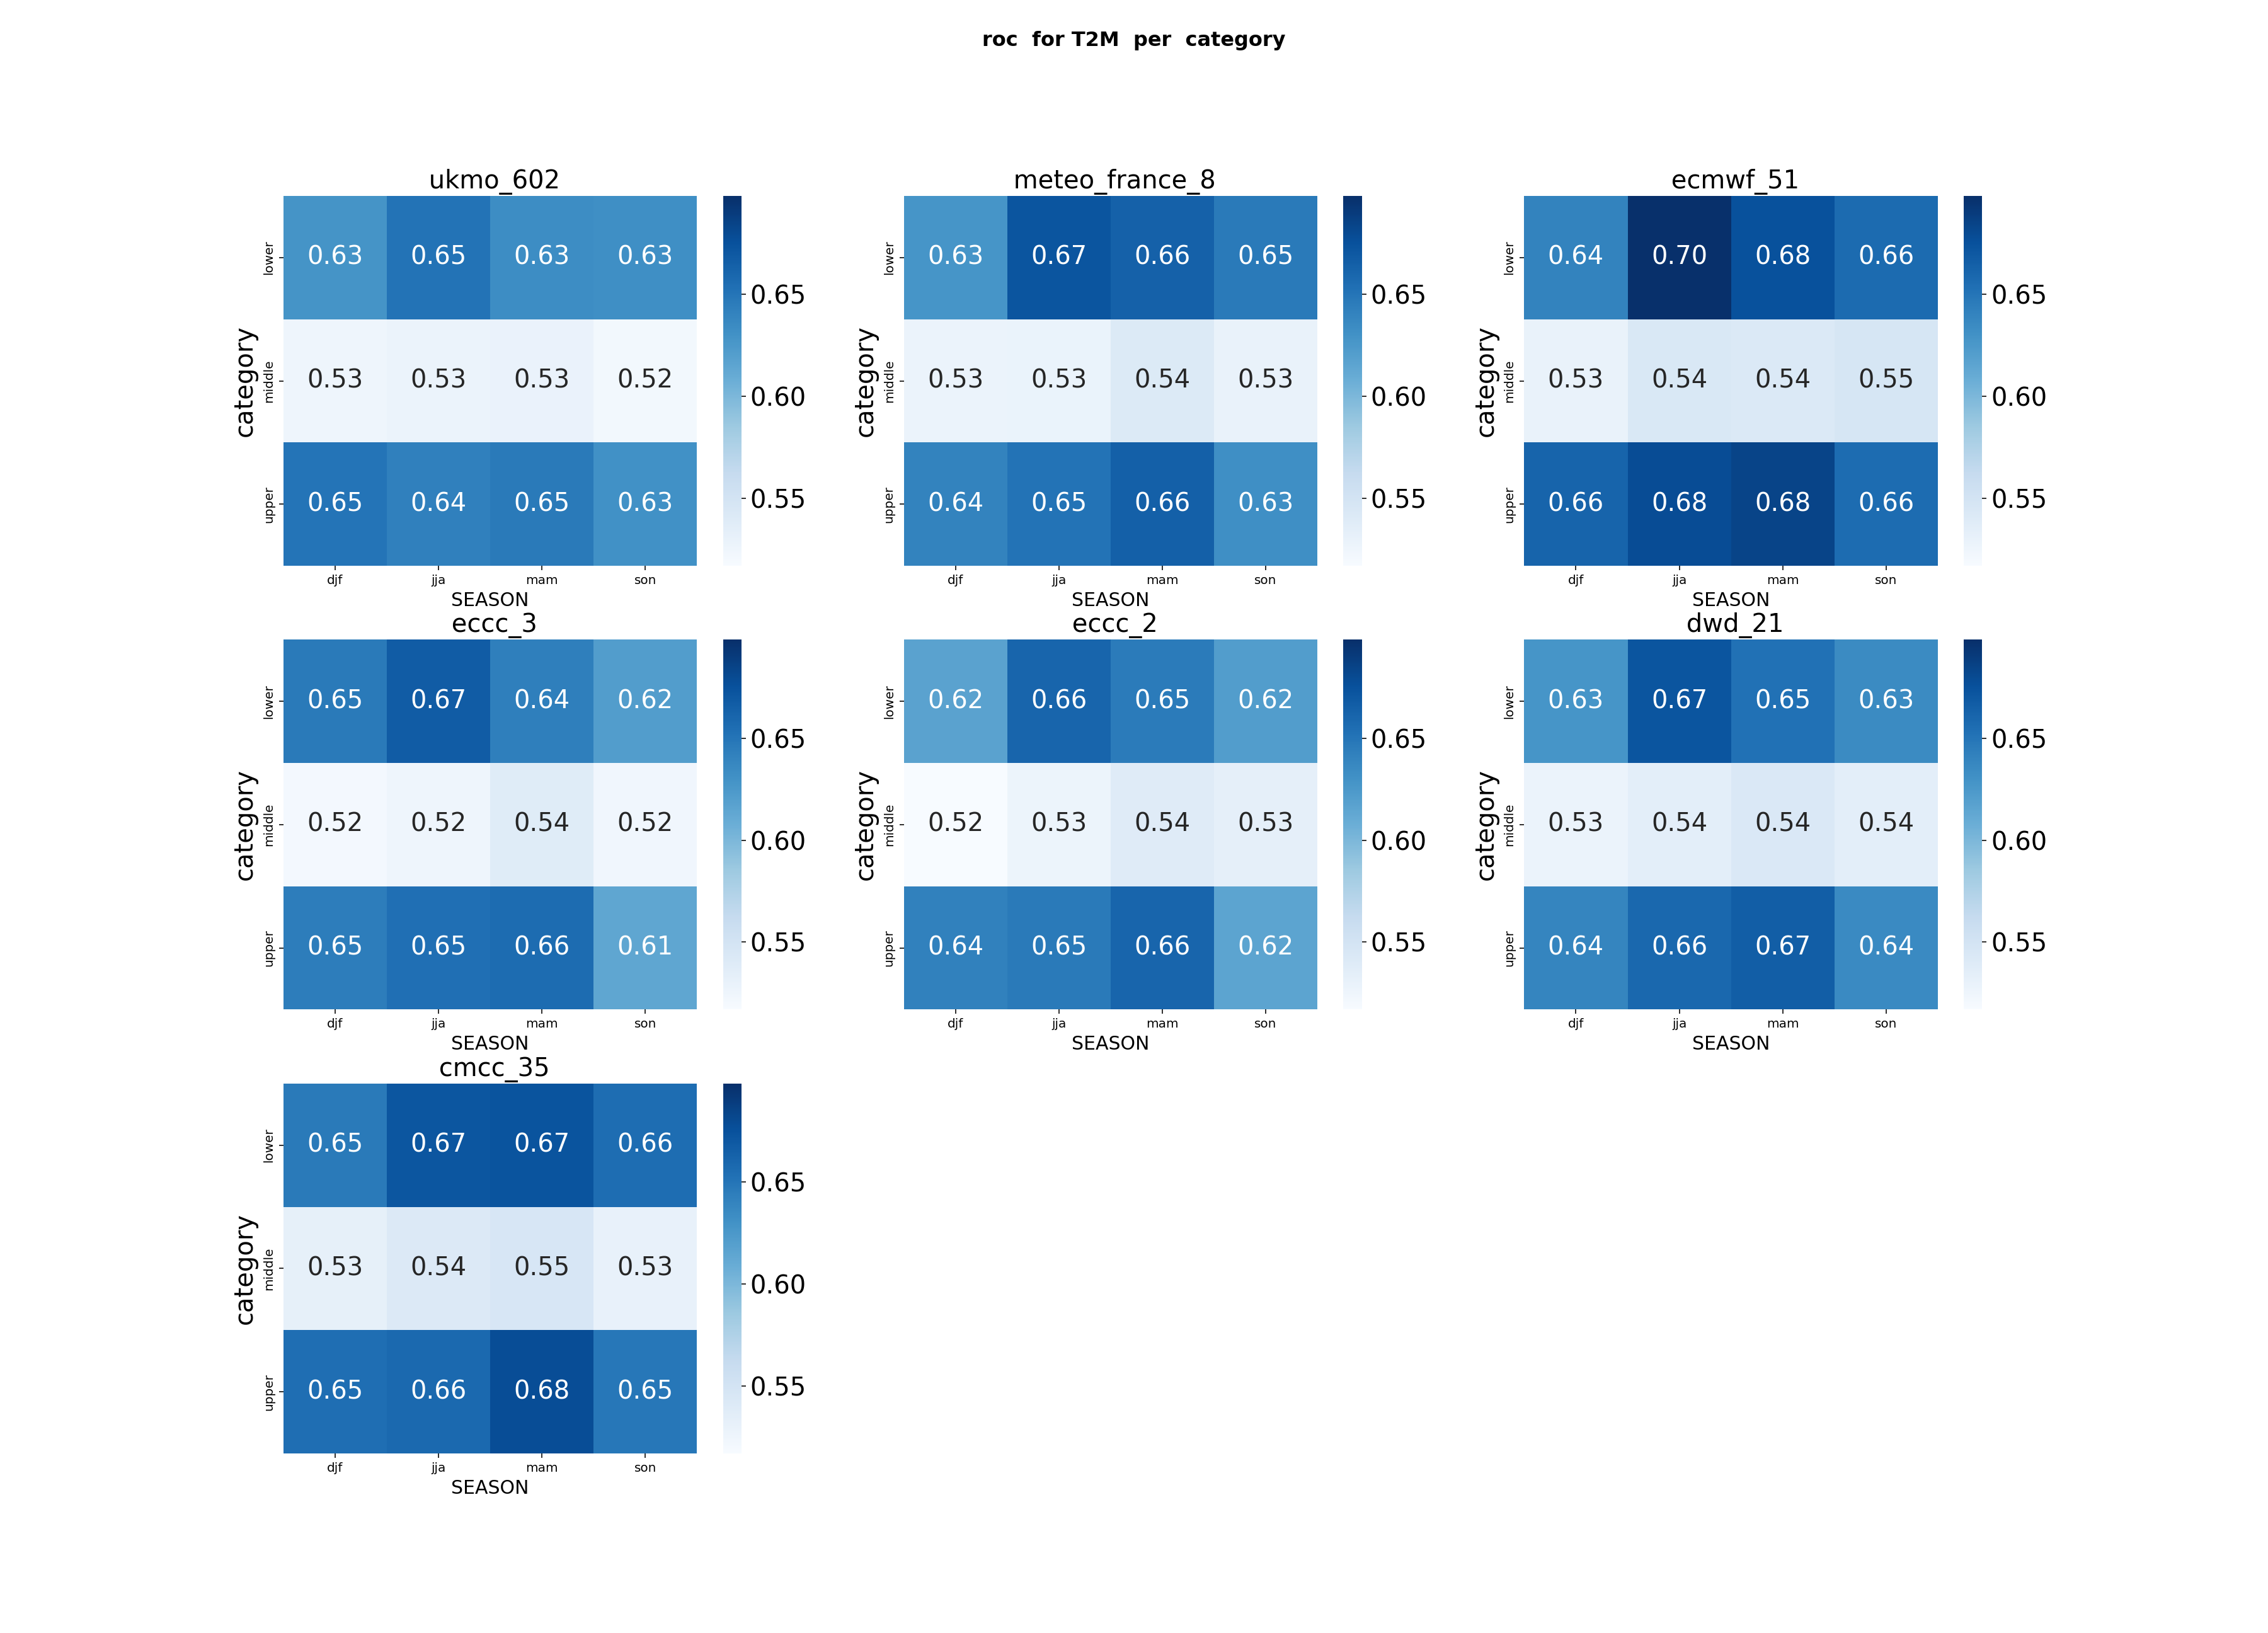
\includegraphics[width=1\linewidth]{plots/prob/roc/roc_T2M_category.png}
    \caption{Temperature AUC  heatmaps }
\end{figure}


Models generally exhibit similar performance, as indicated by the high Area Under the ROC Curve (AUC) values, which reflect their ability to effectively discriminate between predicted probabilities and observed outcomes. Unlike the reliability metric, where UKMO showed weaker performance, it performs relatively well in terms of the AUC, demonstrating good skill in distinguishing between forecasted events and non-events. Similar to the findings with the Brier Score (BS), the "middle" probability category tends to show weaker performance compared to the "lower" and "upper" categories. This highlights the models' greater sensitivity in accurately predicting events with extreme probabilities (high or low), but reduced skill for moderate probability scenarios. This consistency across metrics underscores the need to address forecast performance specifically in the middle category to further improve model predictions.

\begin{figure}[H]
    \centering
    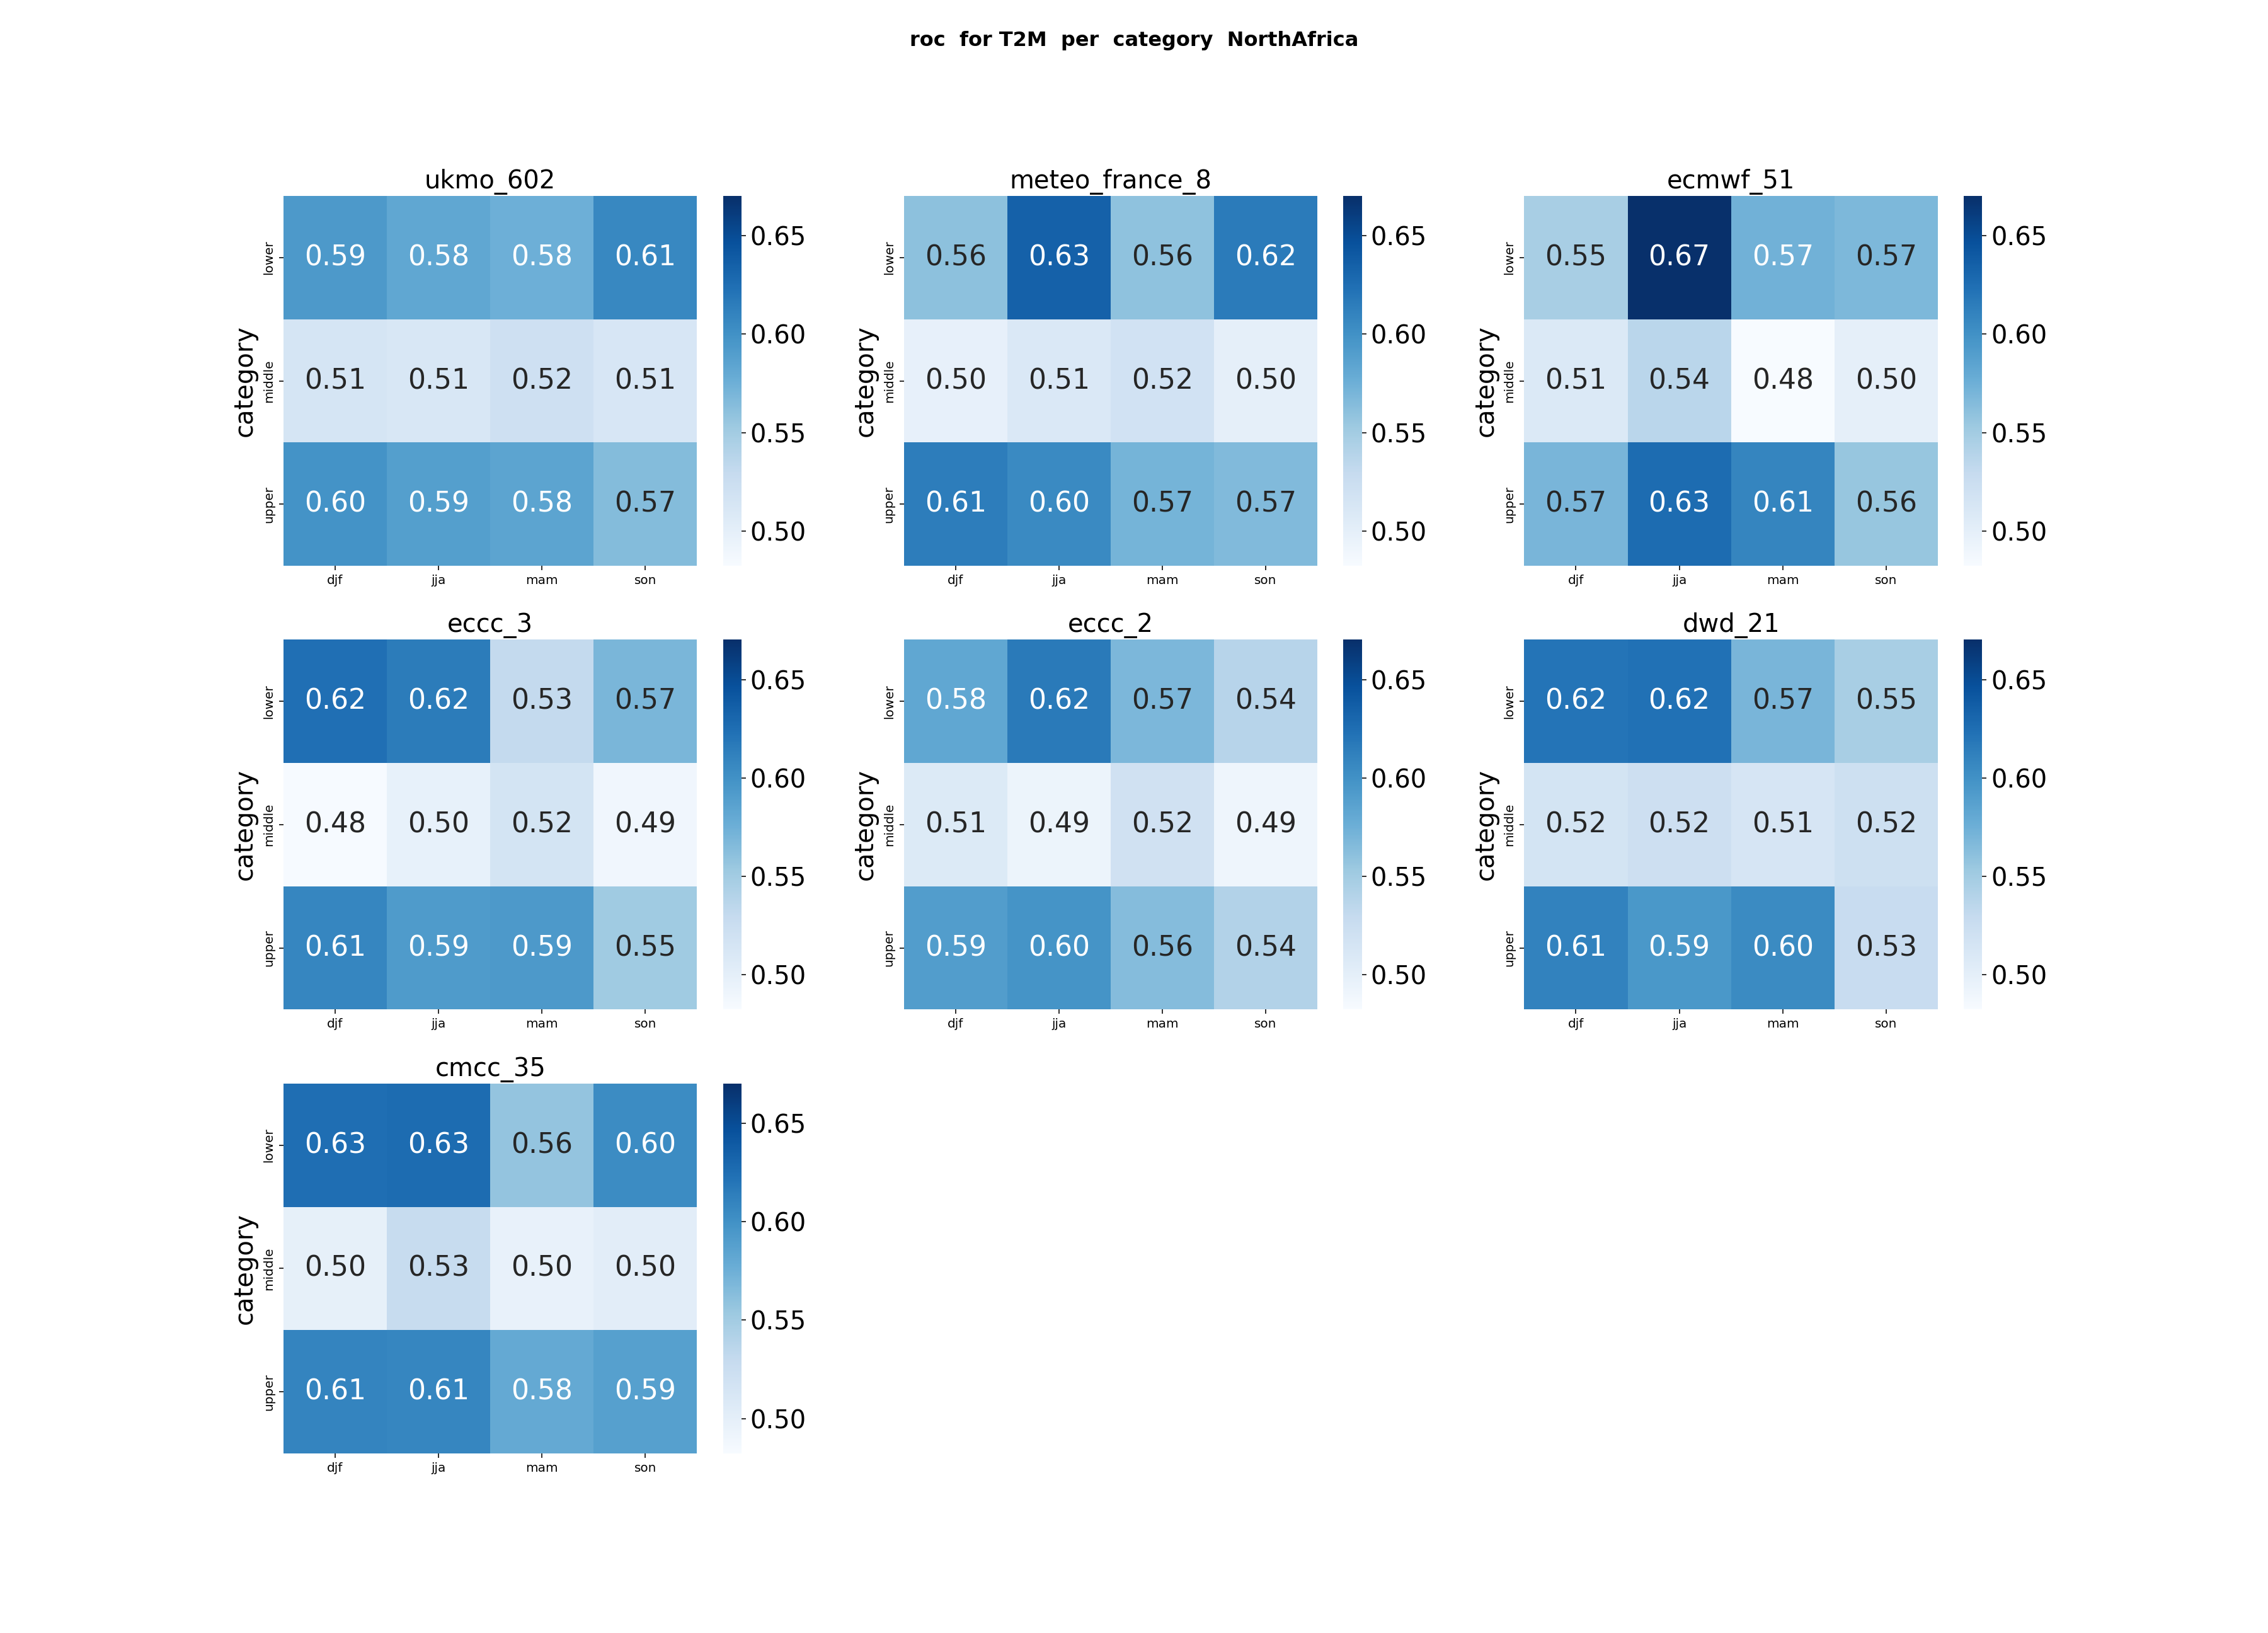
\includegraphics[width=1\linewidth]{plots/prob/roc/roc_T2M_category_NorthAfrica.png}
    \caption{Temperature AUC  heatmaps for north africa }
\end{figure}
The figure above confirms the same conclusions for the North Africa region. The models generally maintain similar performance, with high AUC values reflecting strong discrimination skill across all categories. UKMO continues to show robust results in terms of ROC, despite its weaker reliability performance. As observed previously, the "middle" probability category remains the least performant compared to the "lower" and "upper" categories, indicating the models' reduced ability to predict moderate probability events. This consistency in findings suggests that the regional focus on North Africa does not significantly alter the overall assessment of model performance.
\subsubsection{Relative operating characteristics Skill Score}
ROCSS provides an assessment of a model's ability to discriminate between observed and forecasted events relative to a reference model, often a climatological or random forecast. A higher ROCSS indicates that the model has skill in distinguishing between occurrences and non-occurrences of an event, while a score close to zero suggests no significant improvement over the reference

\begin{figure}[H]
    \centering
    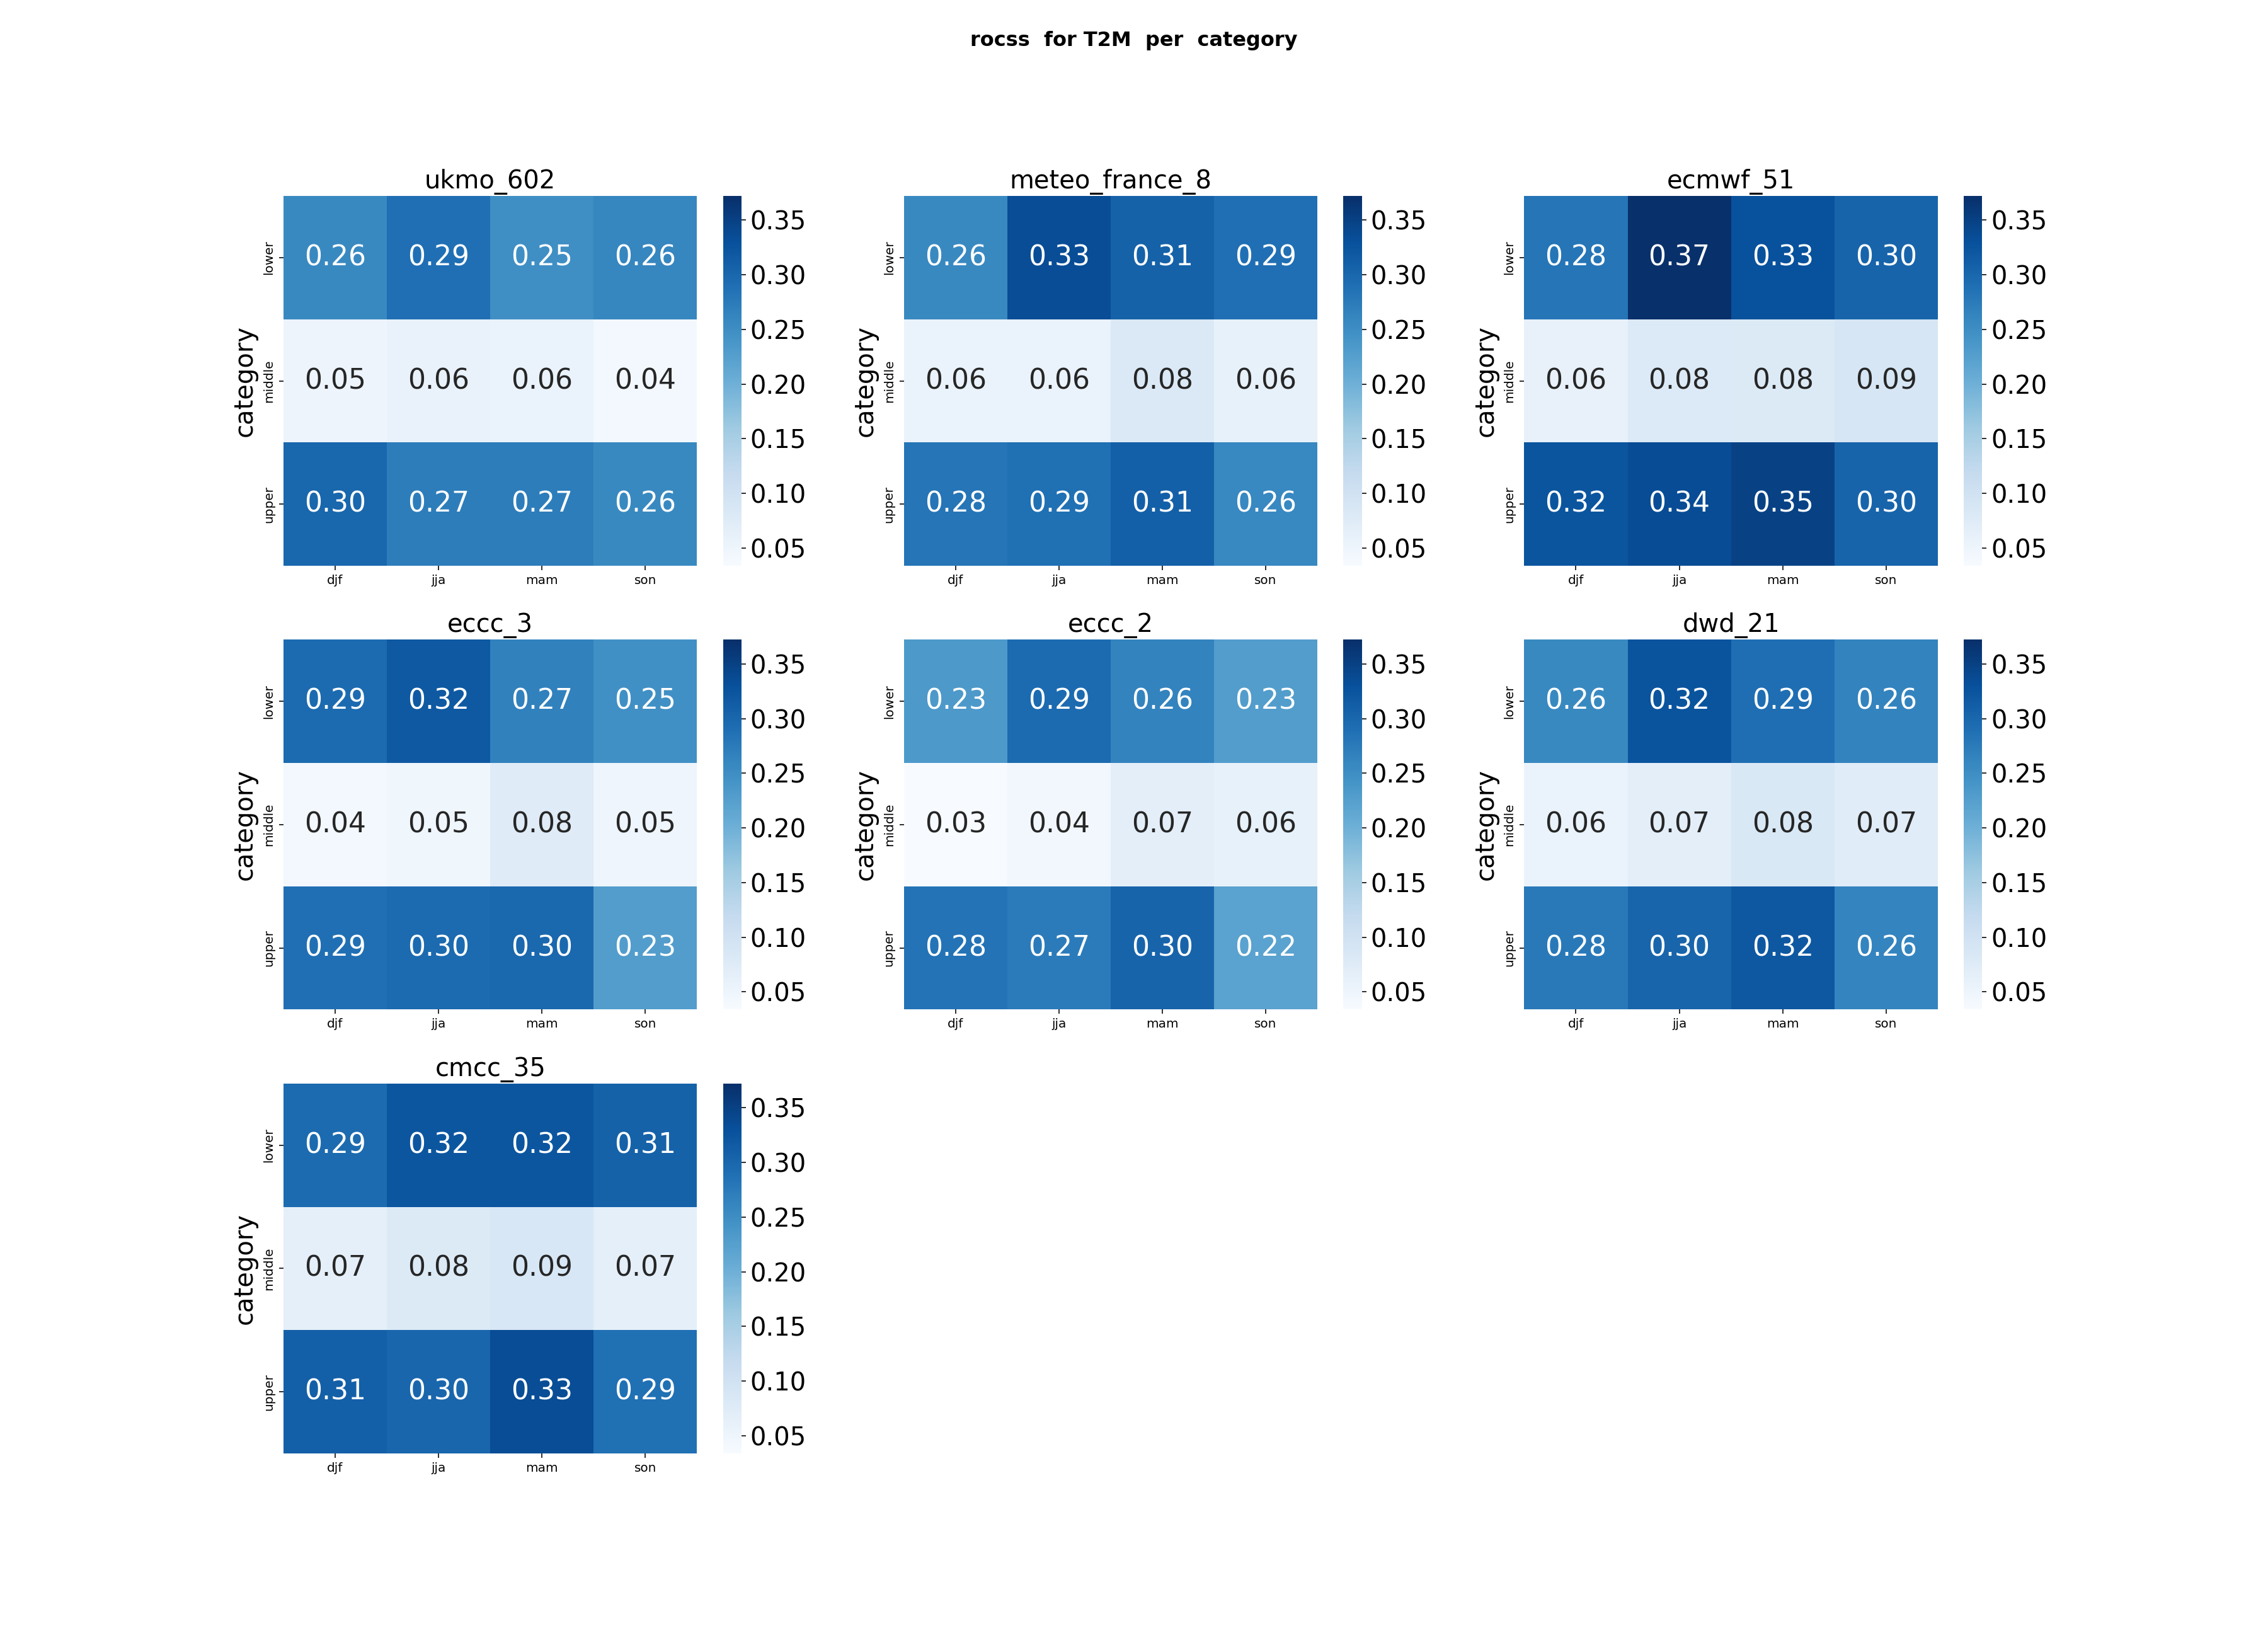
\includegraphics[width=1\linewidth]{plots/prob/rocss/rocss_T2M_category.png}
    \caption{Temperature ROCSS  heatmaps for MENA region }
\end{figure}. 
The ROC Skill Score (ROCSS) analysis reveals similar conclusions to the ROC results for Mena region and north Africa. The models generally demonstrate consistent and positive skill, highlighting their ability to discriminate between observed and forecasted events. UKMO, which showed weaker performance in reliability metrics, continues to perform well in terms of ROCSS, confirming its relative robustness in event discrimination. Additionally, as observed with the ROC scores, the "middle" category exhibits lower performance compared to the "lower" and "upper" categories. This indicates that while the models excel at predicting extreme events with high or low probabilities, their ability to capture moderate probability events remains limited.

\begin{figure}[H]
    \centering
    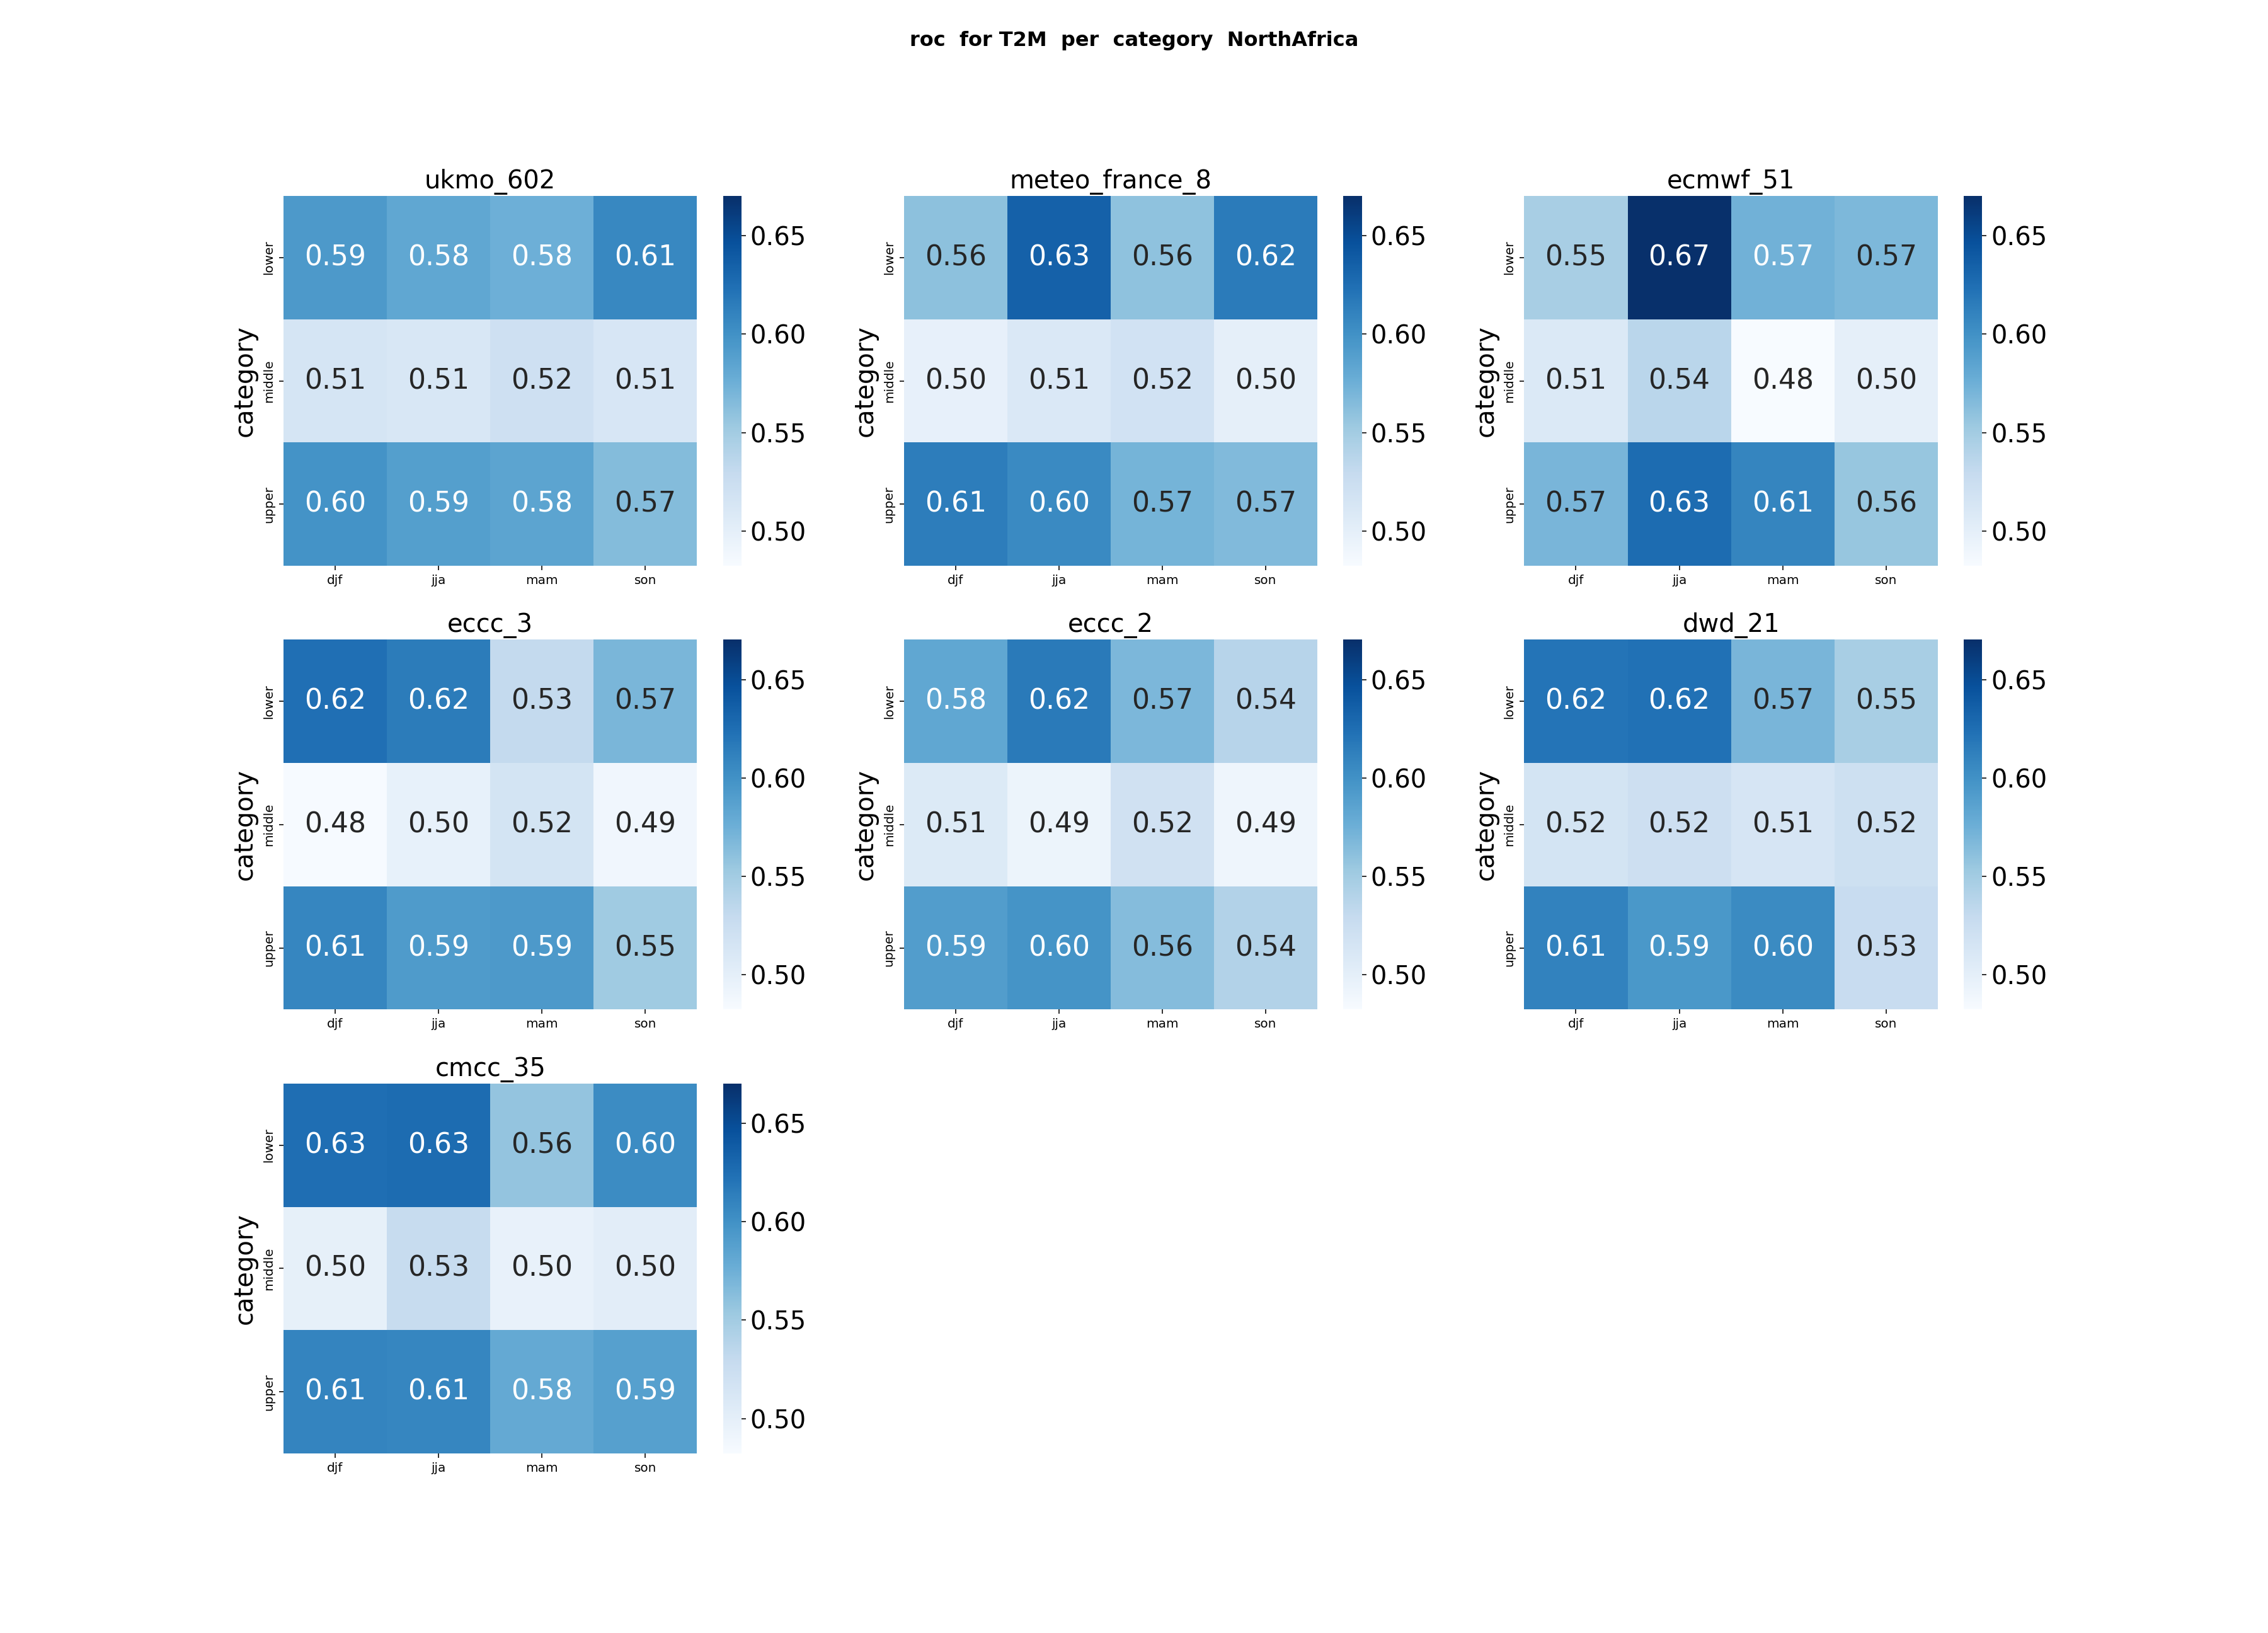
\includegraphics[width=1\linewidth]{plots/prob/roc/roc_T2M_category_NorthAfrica.png}
    \caption{Temperature ROCSS  heatmaps for north africa }
\end{figure}






\section{PRECIPITATIONS}
IN general, the forecast of precipitations is more complicated than temperature, thus the scores are a little less good for this part especially the deterministic ones. 
\subsection{Deterministic Evaluation Metrics}

\subsubsection{Spearman rank correlation}

\begin{figure}[H]
	\centering
	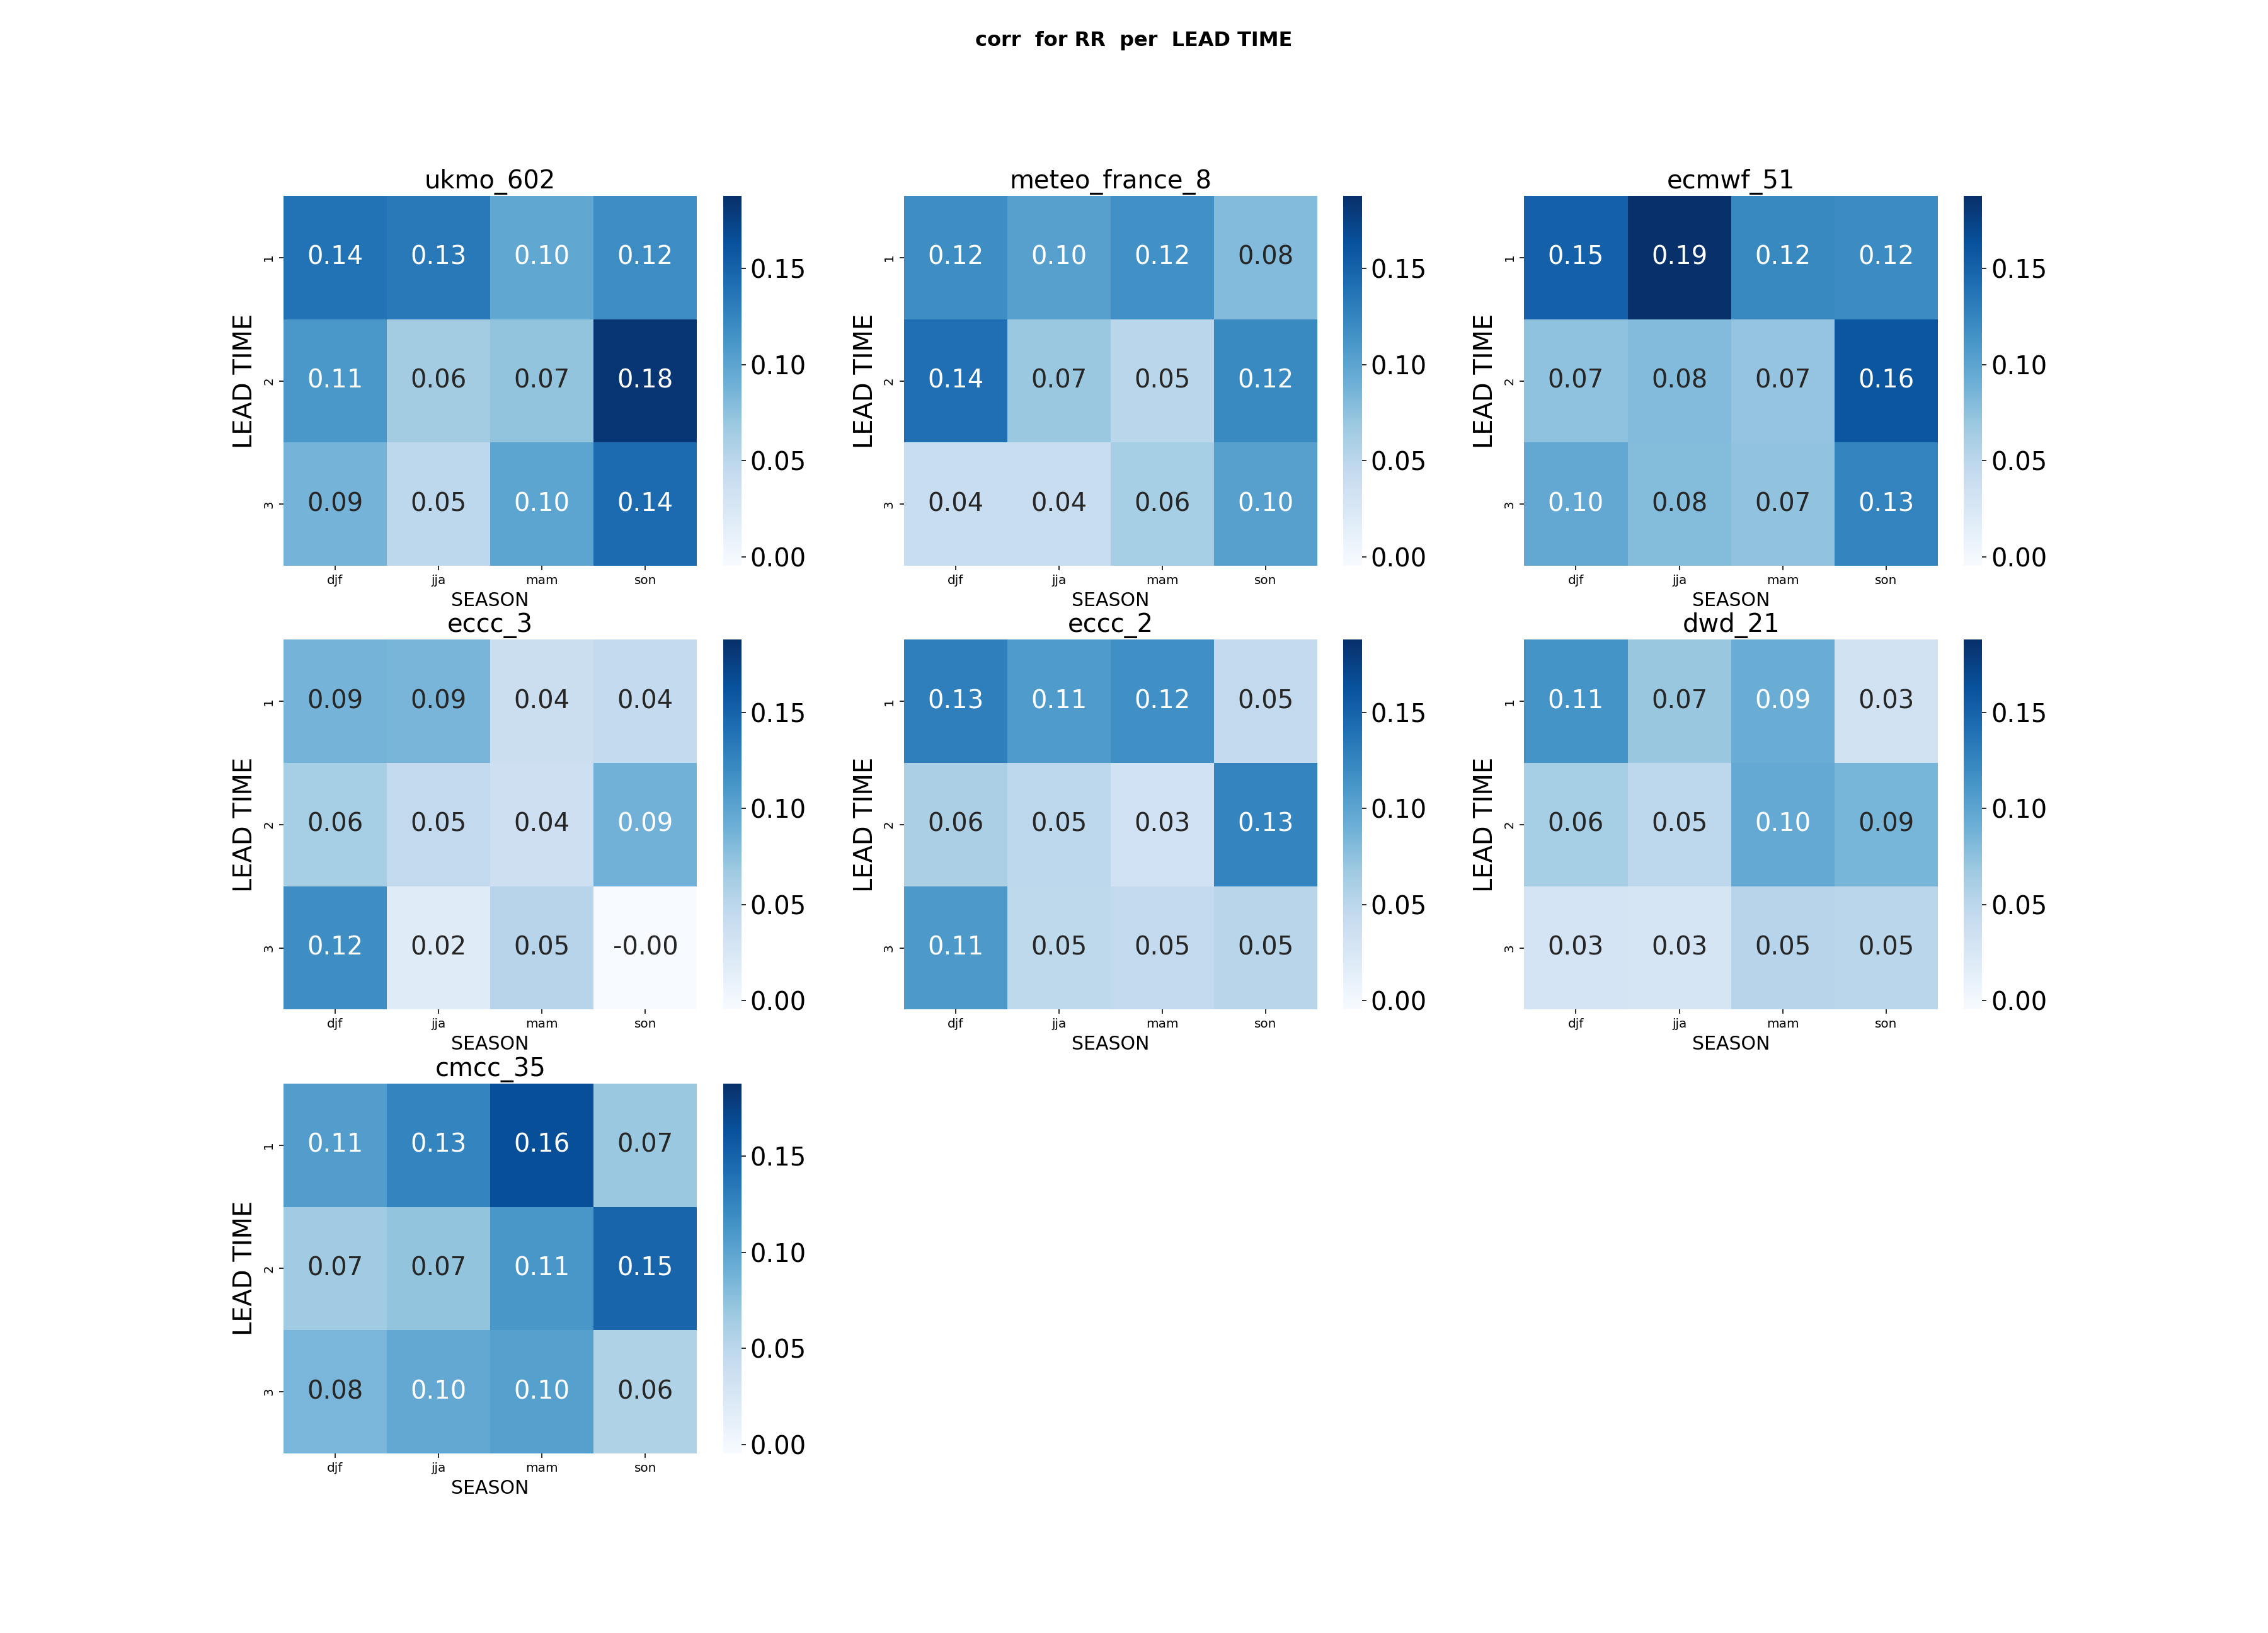
\includegraphics[scale=0.25]{plots/det/corr/corr_RR.png}
	\caption{The Heatmap of correlation for the mena region for every period \textbf{\textit{(1 for perfect Correlation)} }}
\end{figure}
The correlation is weak for all centers; however, the best models are \textbf{\textit{ECMWF, UKMO, and CMCC-35}}. There is no clear variability in performance along lead-time. For SON, the performance is excellent at lead-time 2 for all centers. As for the other seasons, the performance is generally strong at the 1st lead-time but decreases with increasing lead-time.
Hence, Meteo-France also shows good performance, but it decreases significantly over time.



\begin{figure}[H]
\centering
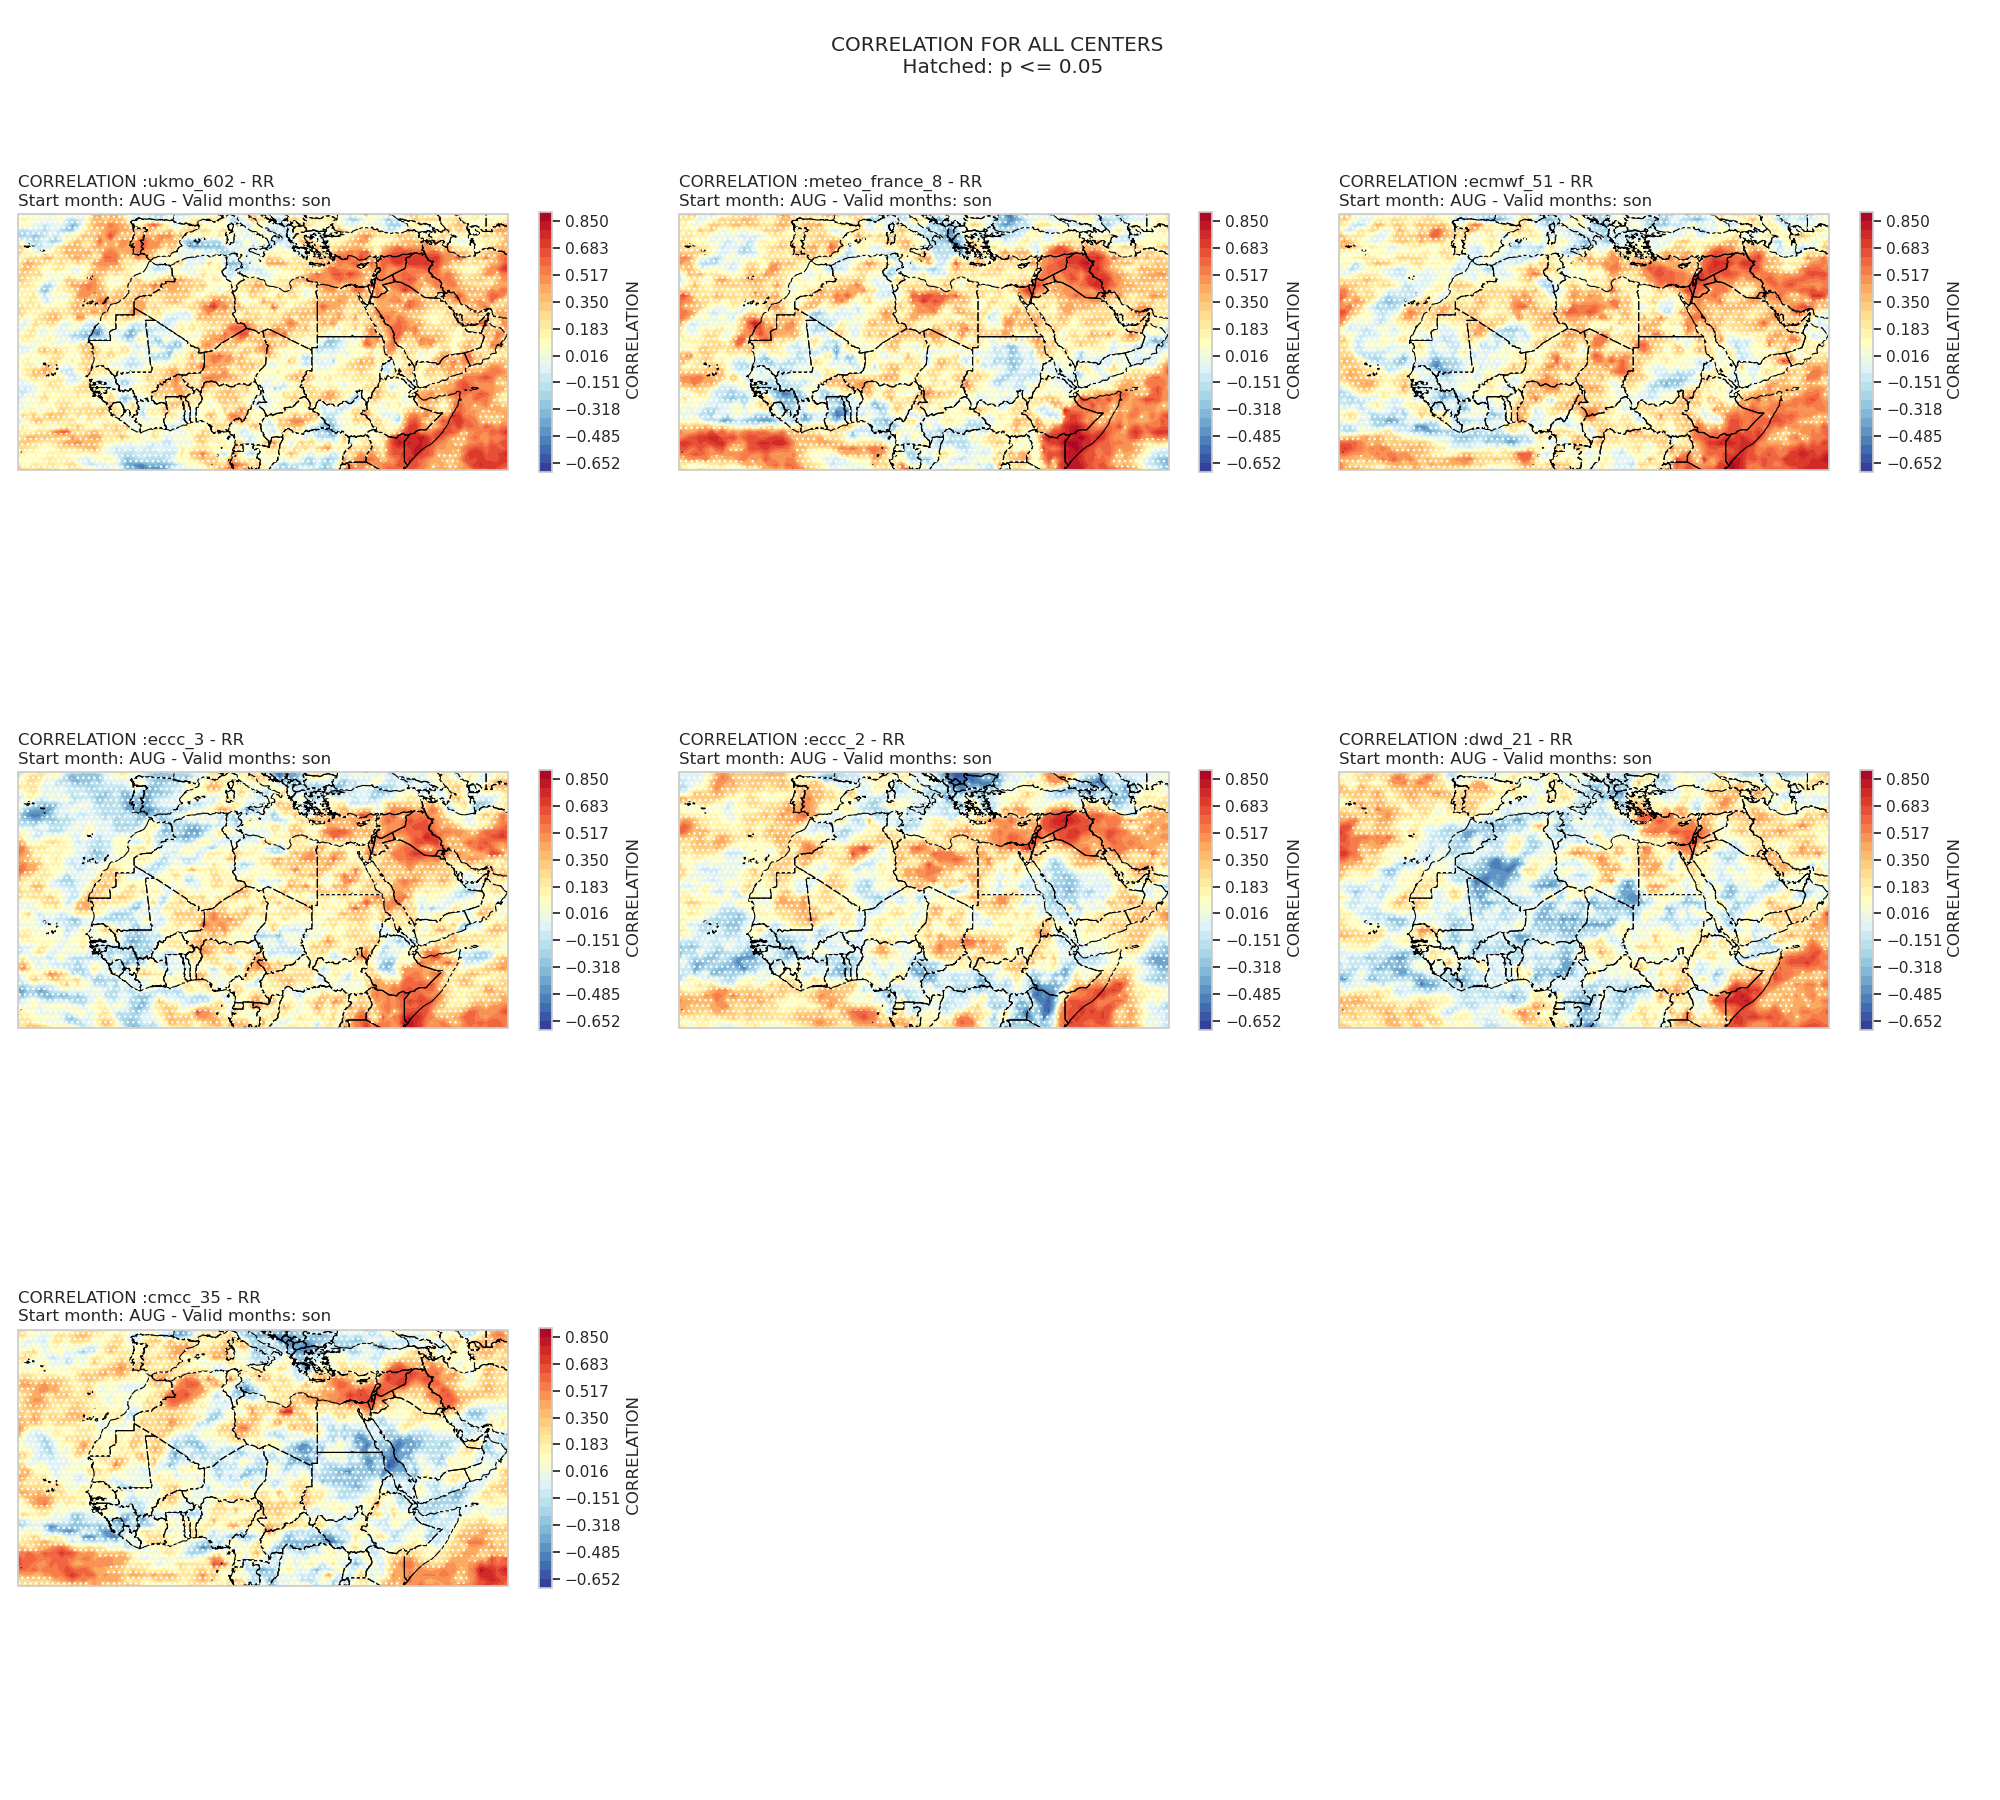
\includegraphics[scale=0.3]{plots/det/corr/CORR_son_RR.png}
\caption{3-months Rolling mean of Spearman Correlation in MENA Region for all centers SON}
\end{figure}
For temperature, the models demonstrate the best performance in the tropical regions. However, for precipitation, the situation is different. Hence the results show good performance during SON, where the Middle East, East Africa, and North Africa exhibit the highest correlation performance.
\begin{figure}[H]
\centering
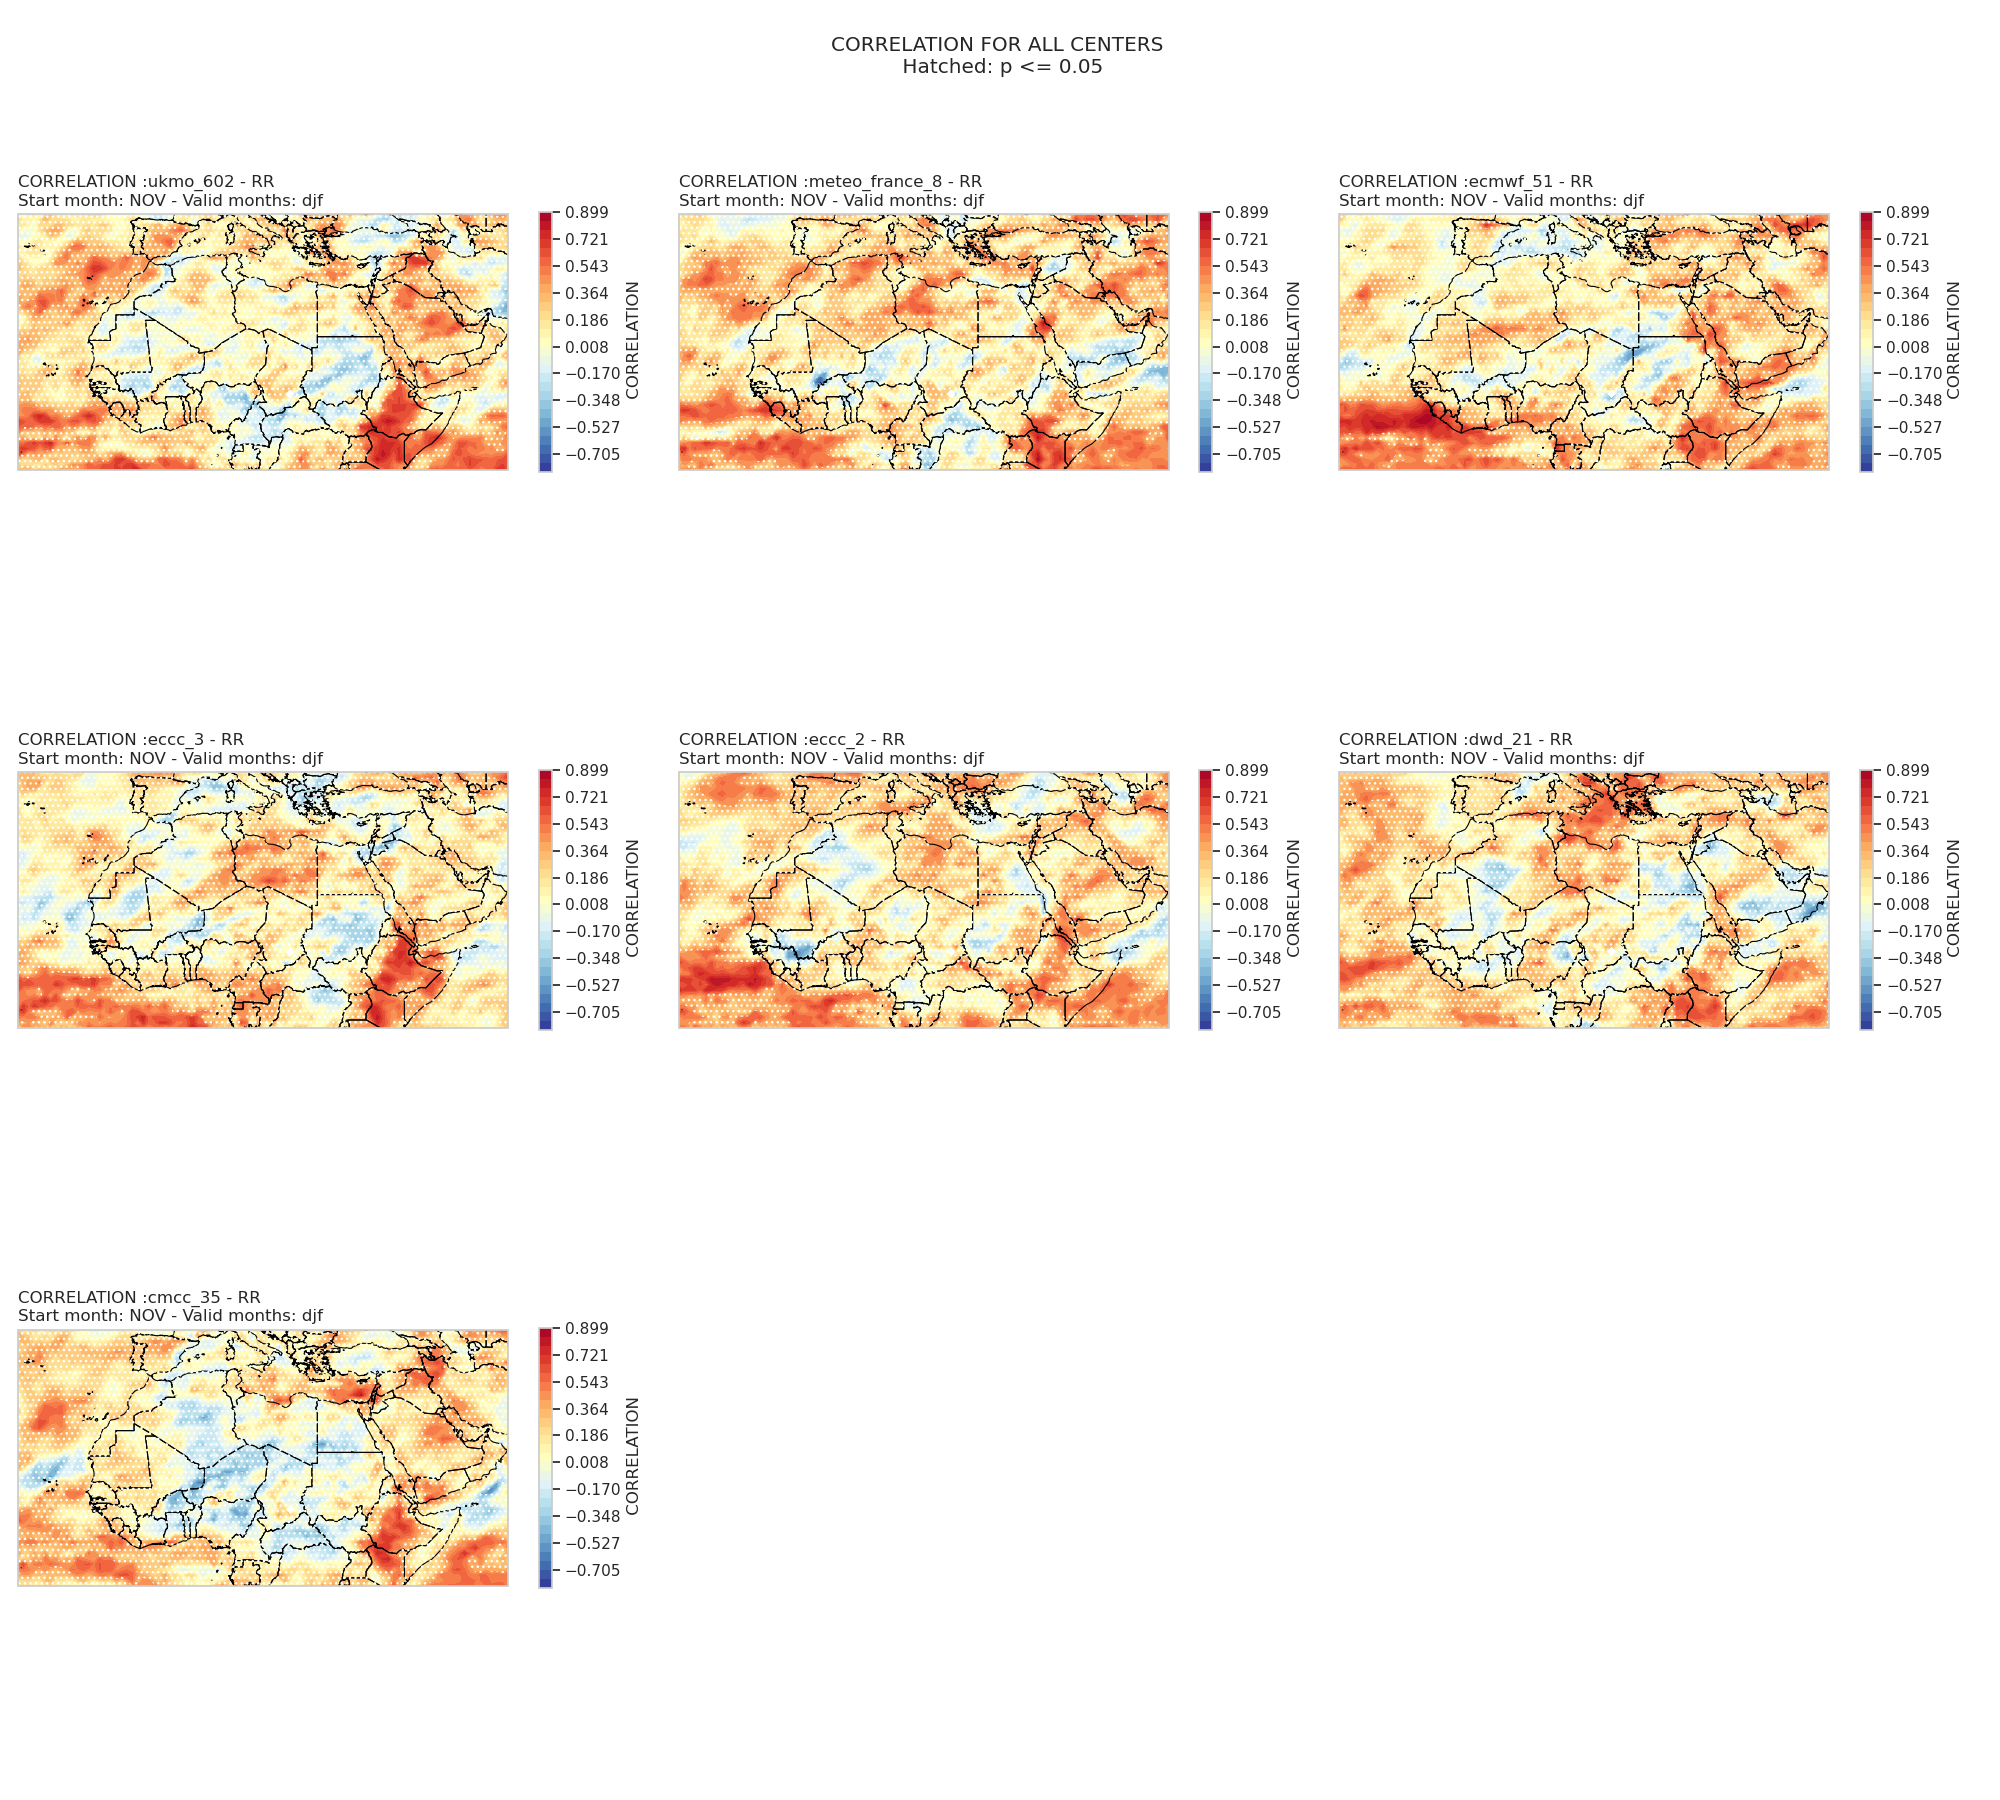
\includegraphics[scale=0.3]{plots/det/corr/CORR_djf_RR.png}
\caption{3-months Rolling mean of Spearman Correlation in MENA Region for all centers DJF}
\end{figure}

The 3-month rolling mean for SON correlation shows that the best models are \textbf{\textit{ECMWF, UKMO, and Meteo-France}}. The correlation is significant across most of the MENA region, except in the east of Africa, Palestine, Syria, Jordan, and Iraq, where the correlation is maximal, for all centers the Middle East and East of Africa are have the highest score. However, near the equator, the correlation is negative and weak. This results are confirmed in all centers.
 
For DJF, the situation is generally better than for SON. The best model for North Africa is \textbf{\textit{Meteo-France}}, as it shows good and significant correlation. In general, \textbf{\textit{ECMWF and Meteo-France}} are the best. In general we notice that there is differences between centers, especially in the Middle East and Center Africa.


\textbf{focus on north africa:}
according to the heatmap below, there is no big difference in term of correlation in North africa.


\begin{figure}[H]
	\centering
	\includegraphics[scale=0.25]{plots/det/corr/corr_RR_NorthAfrica.png}
	\caption{The Heatmap of correlation for the mena region for every period \textbf{\textit{(1 for perfect Correlation)} }}
\end{figure}


\subsubsection{RMSE}
 
for the Root Mean Squared Error, the best models shown in the heatmap below are \textbf{\textit{DWD, ECMWF and UKMO}}. The RMSE score demonstrate an excellent performance for all models especially \textbf{\textit{DWD, ECMWF and UKMO}}. The performance is stable over lead-times and it is much better for djf in all centers.

\begin{figure}[H]
\centering
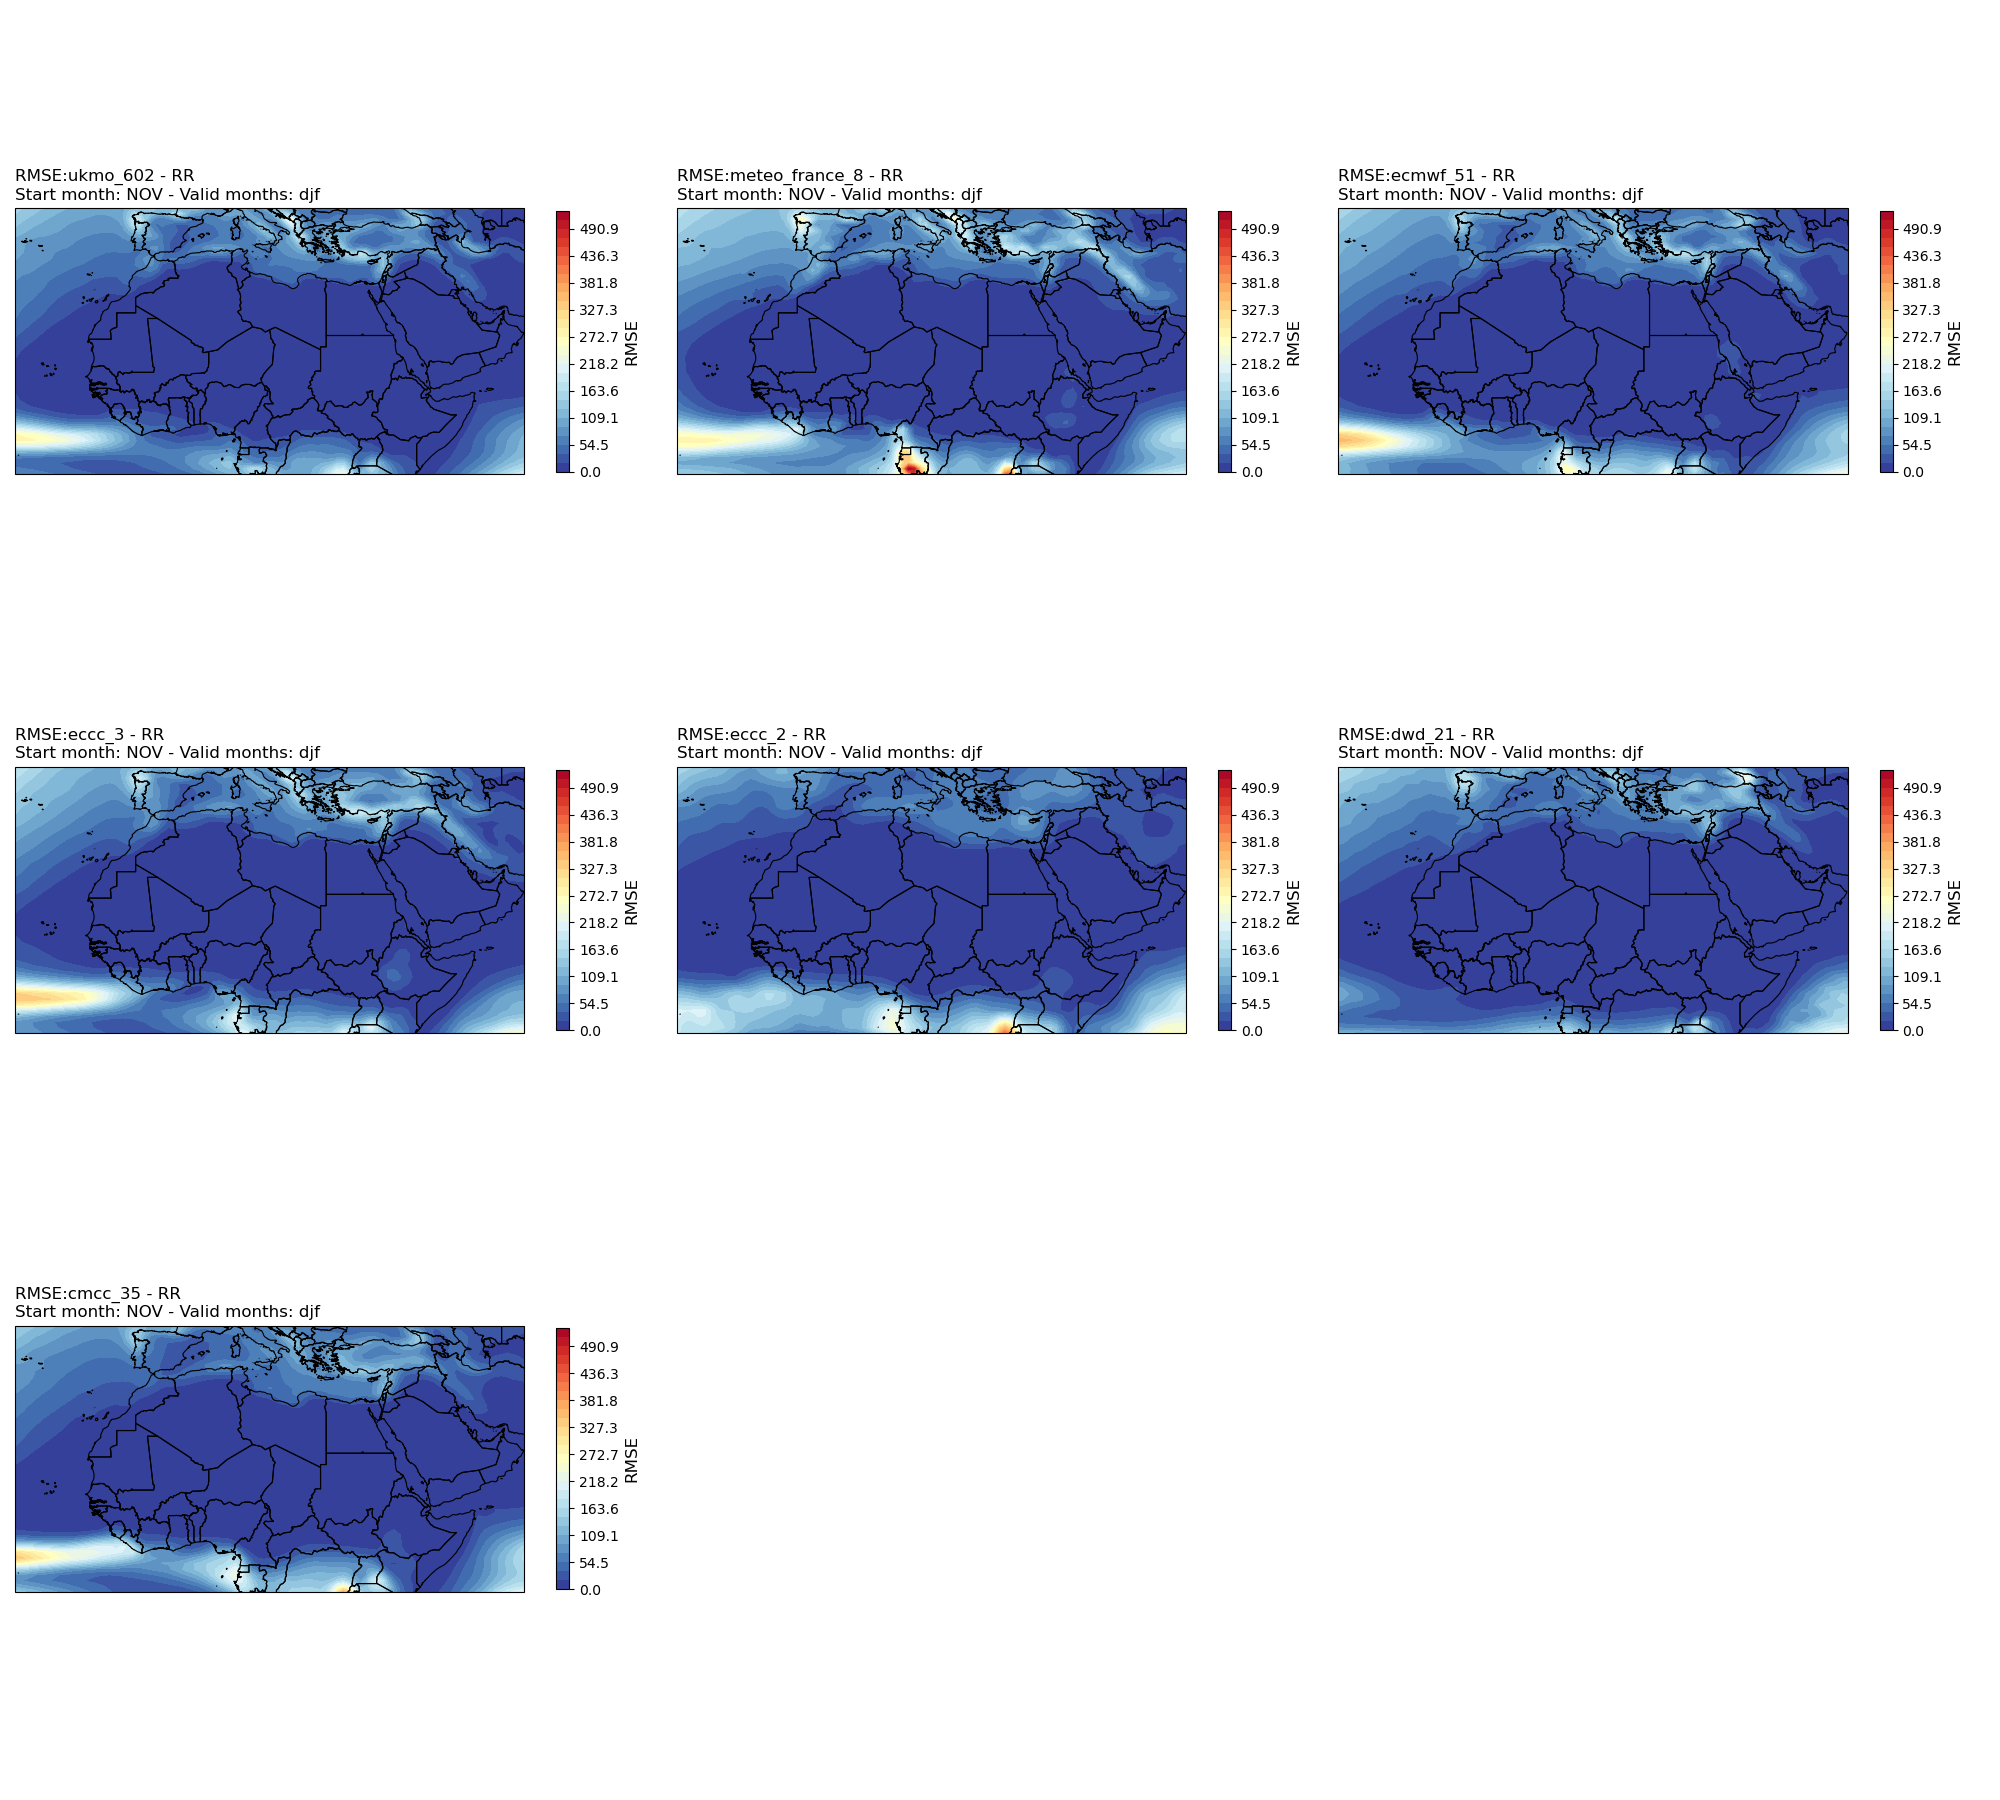
\includegraphics[scale=0.3]{plots/det/rmse/rmse_djf_RR.png}
\caption{3-months Rolling mean of RMSE in MENA Region for all centers DJF}
\end{figure}

\begin{figure}[H]
\centering
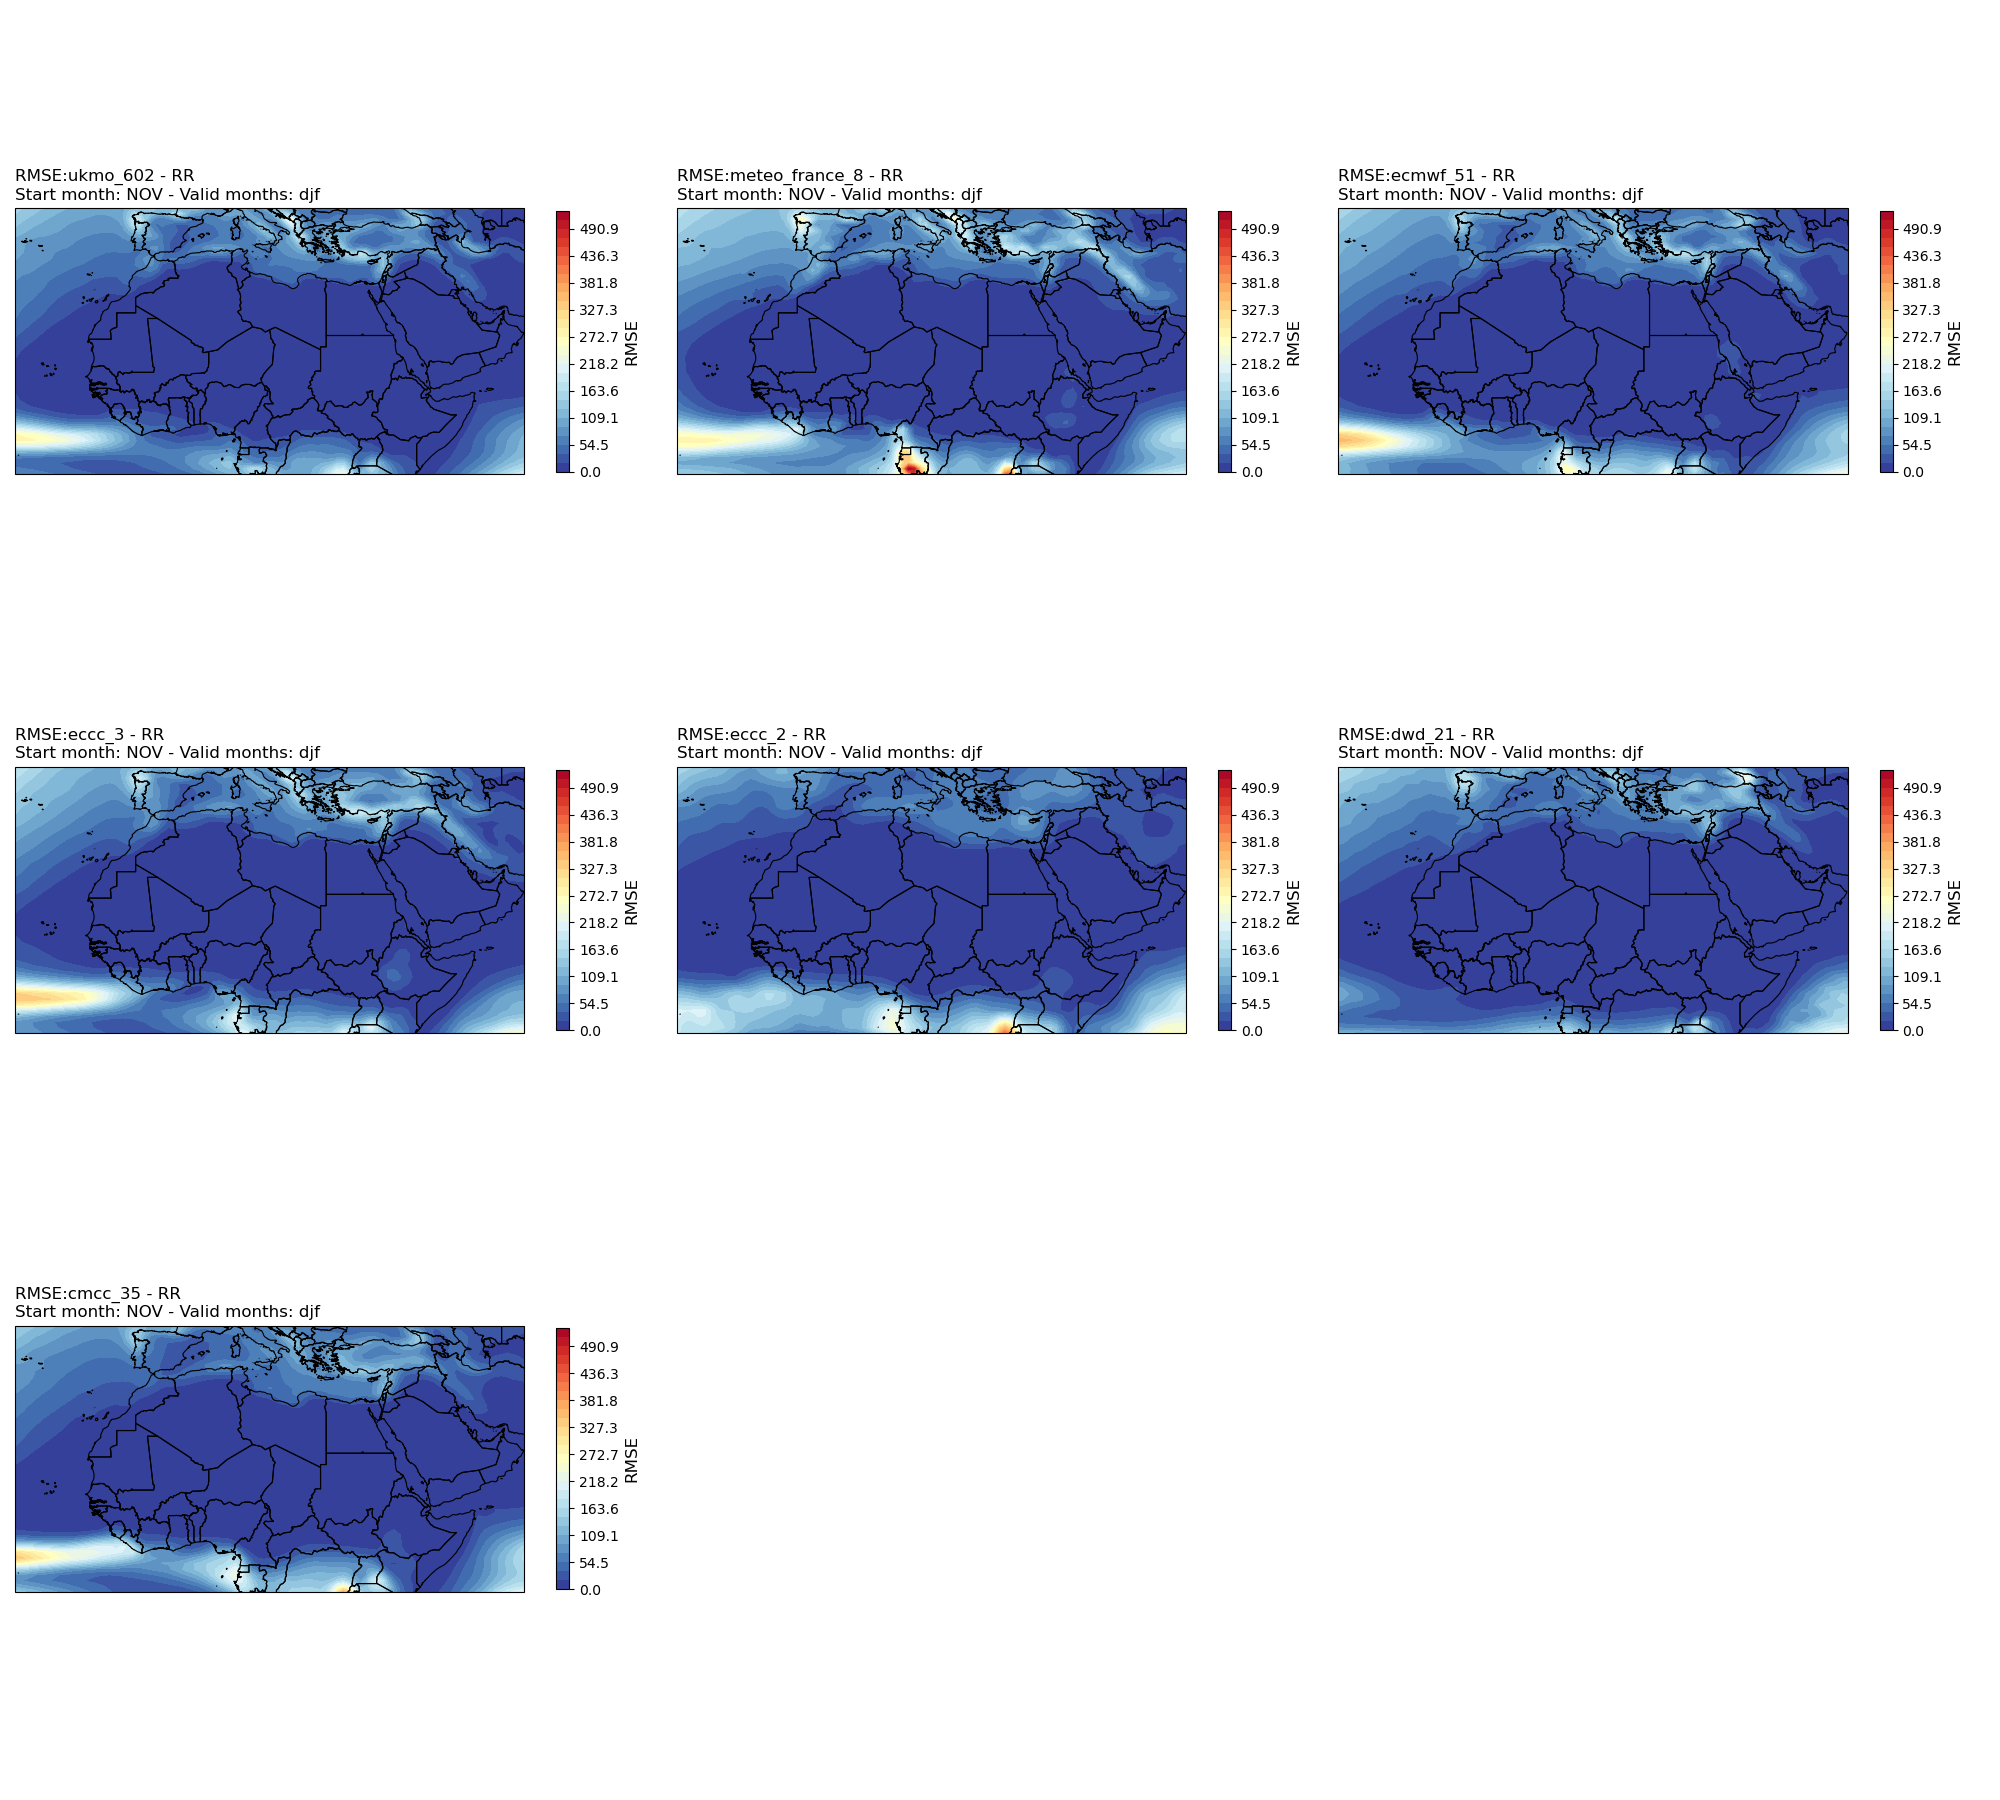
\includegraphics[scale=0.3]{plots/det/rmse/rmse_djf_RR.png}
\caption{3-months Rolling mean of RMSE in MENA Region for all centers JJA}
\end{figure}

also for the spacial dimension, the RMSE stay stable and exhibit very good performance for all centers. Thus, all models have high skill and they are consistent with each other.


\subsubsection{Coefficient of Determination (\( R^2 \))}
for precipitation, the R-SQUARED is very low, the maximum value is less than 0.1. However, the ecmwf is the best in term of R-SQUARED. for DJF,JJA and MAM the highest performance is in the first Lead-time, and it decrease along time, But for SON the best score is in the second Lead-time for all centers.
\begin{figure}[H]
	\centering
	\includegraphics[scale=0.25]{plots/det/rsquared/rsquared_RR.png}
	\caption{The Heatmap of rsquared for Precipitations in the mena region for every period \textbf{\textit{(1 for perfect RSQUARED)} }}
\end{figure}



\begin{figure}[H]
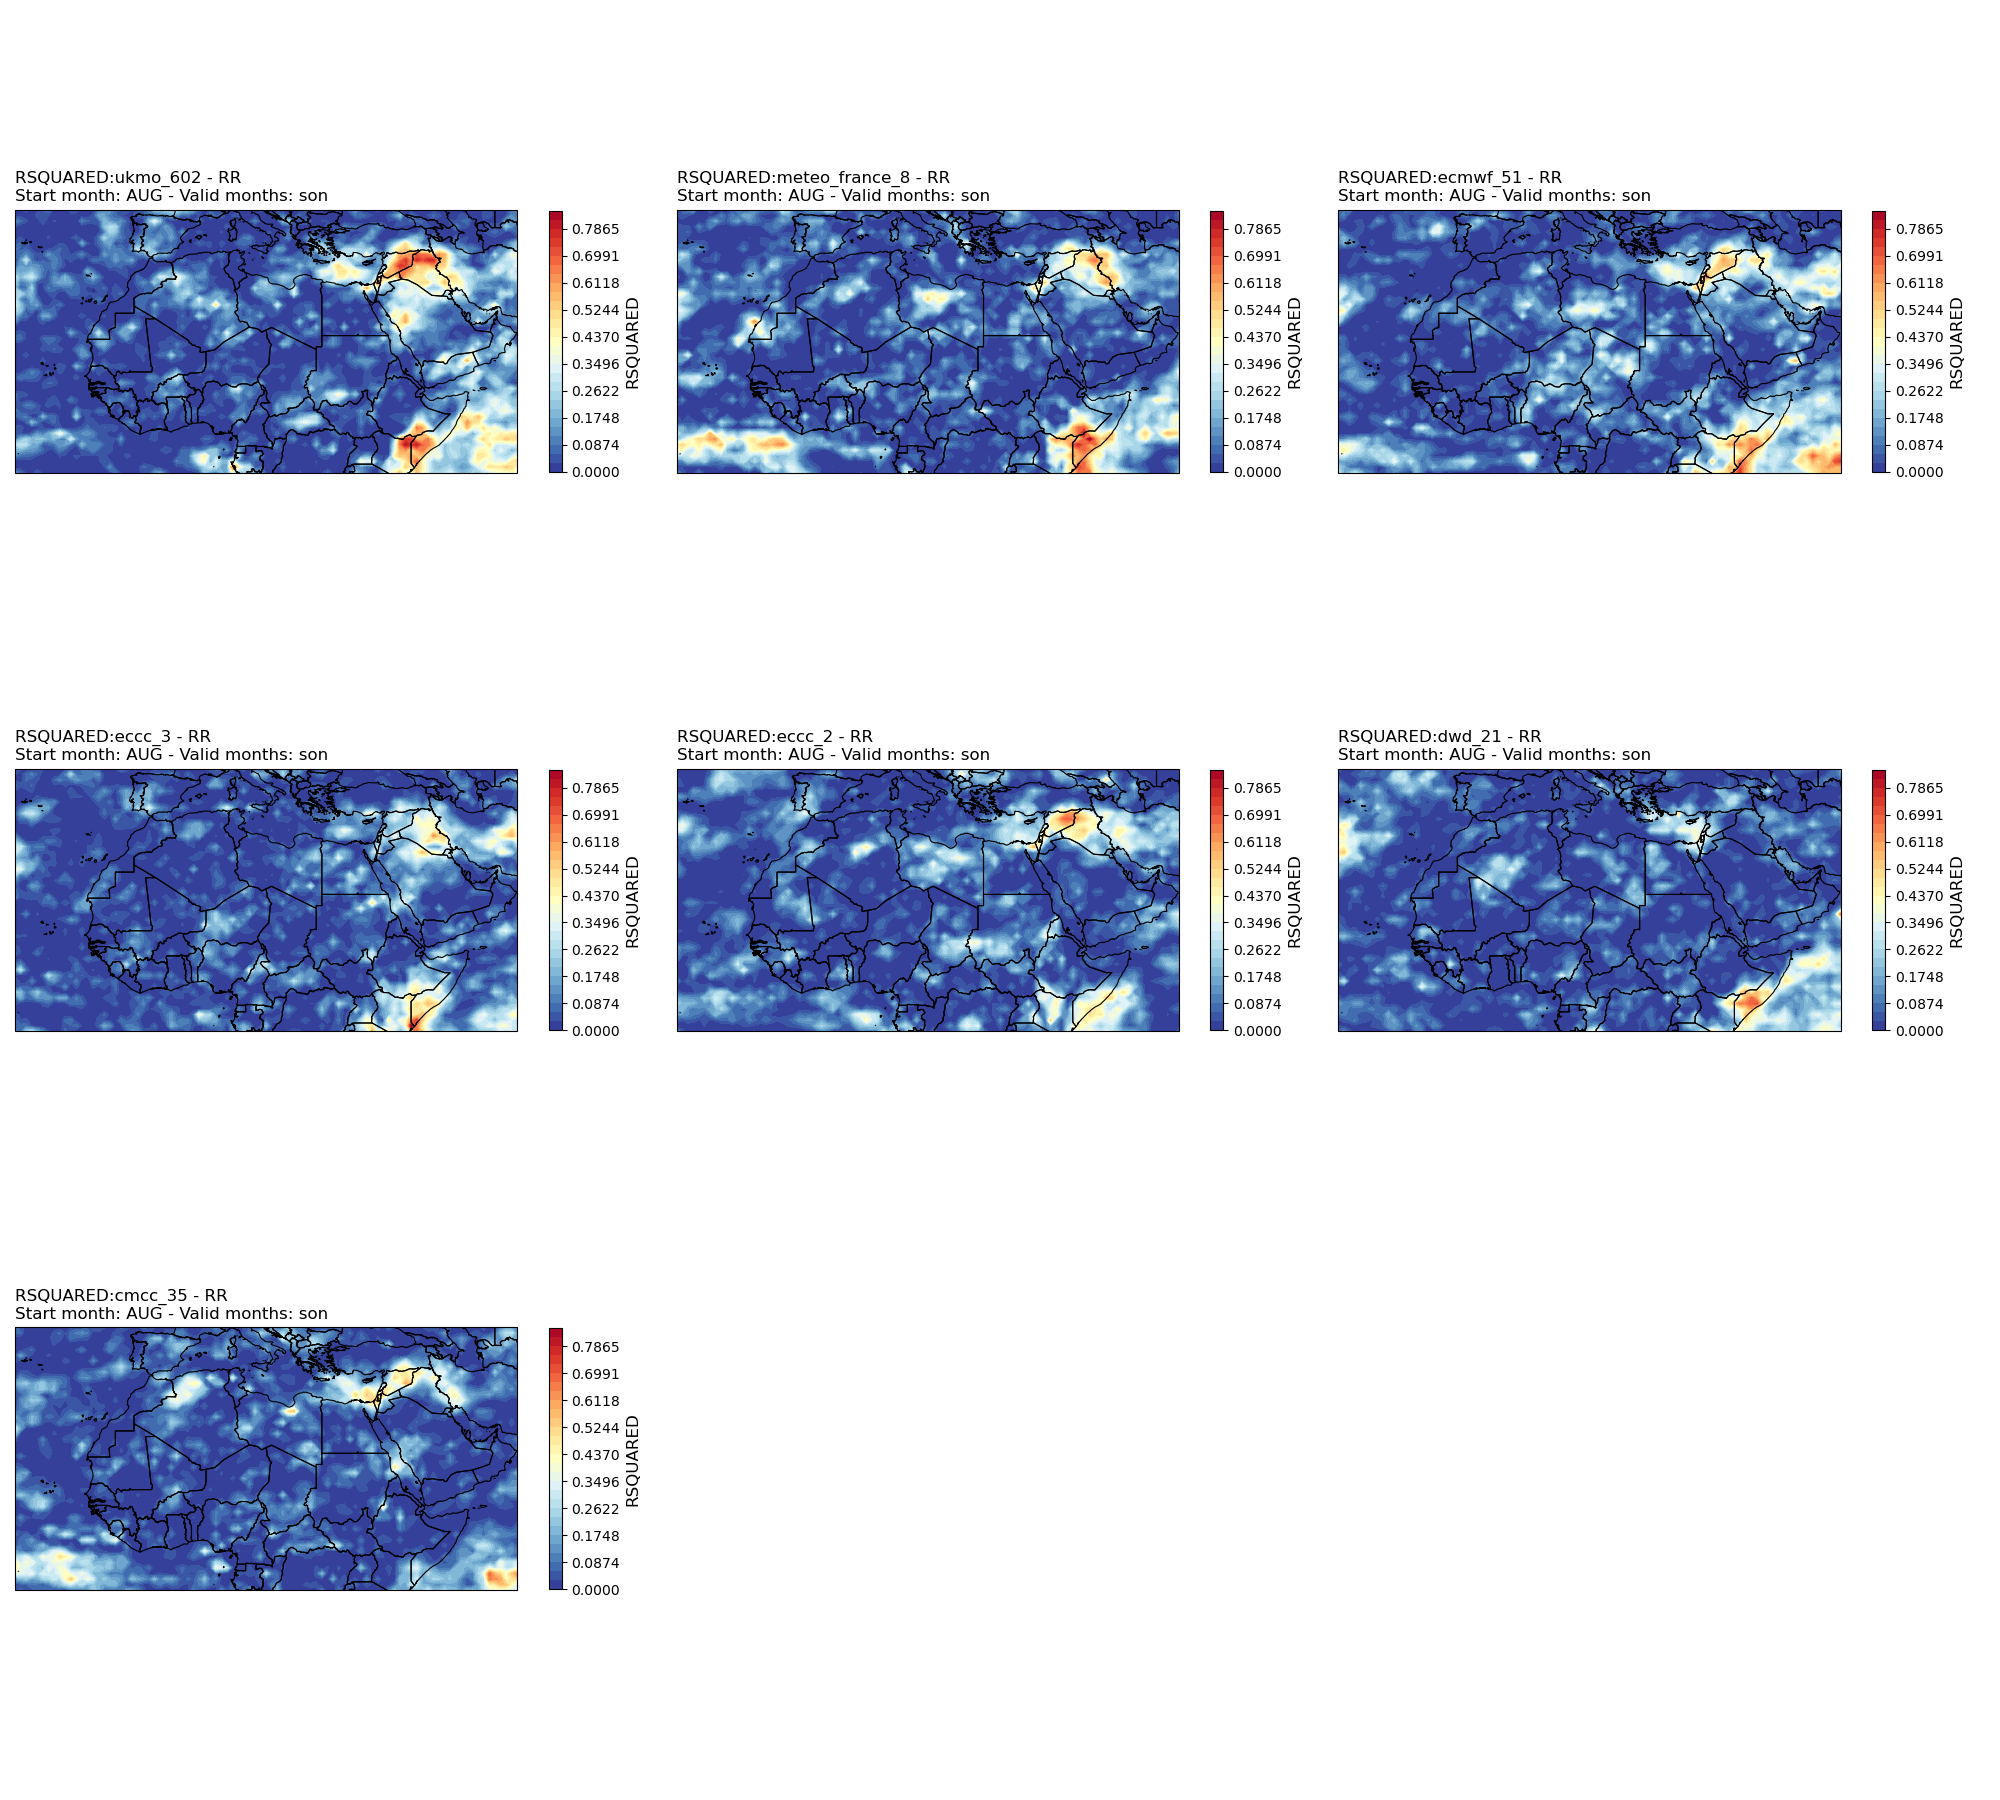
\includegraphics[scale=0.3]{plots/det/rsquared/rsquared_son_RR.png}
\caption{3-months Rolling mean of RSQUARED in MENA Region for all centers SON}
\end{figure}

there is some isolated zones where the r-squared is good especially in Syria, Irak, Jordan ,Palestine  and East Africa, this high performance is observed in all centers. For the rest of the MENA region the performance is very bad with score near to 0. Hence, there is no constant pattern for the R-SQUARED, the spacial variation is very high for all centers.


\subsection{Probabilistic Evaluation Metrics}

\subsubsection{The Brier Score (BS)}

\begin{figure}[H]
    \centering
    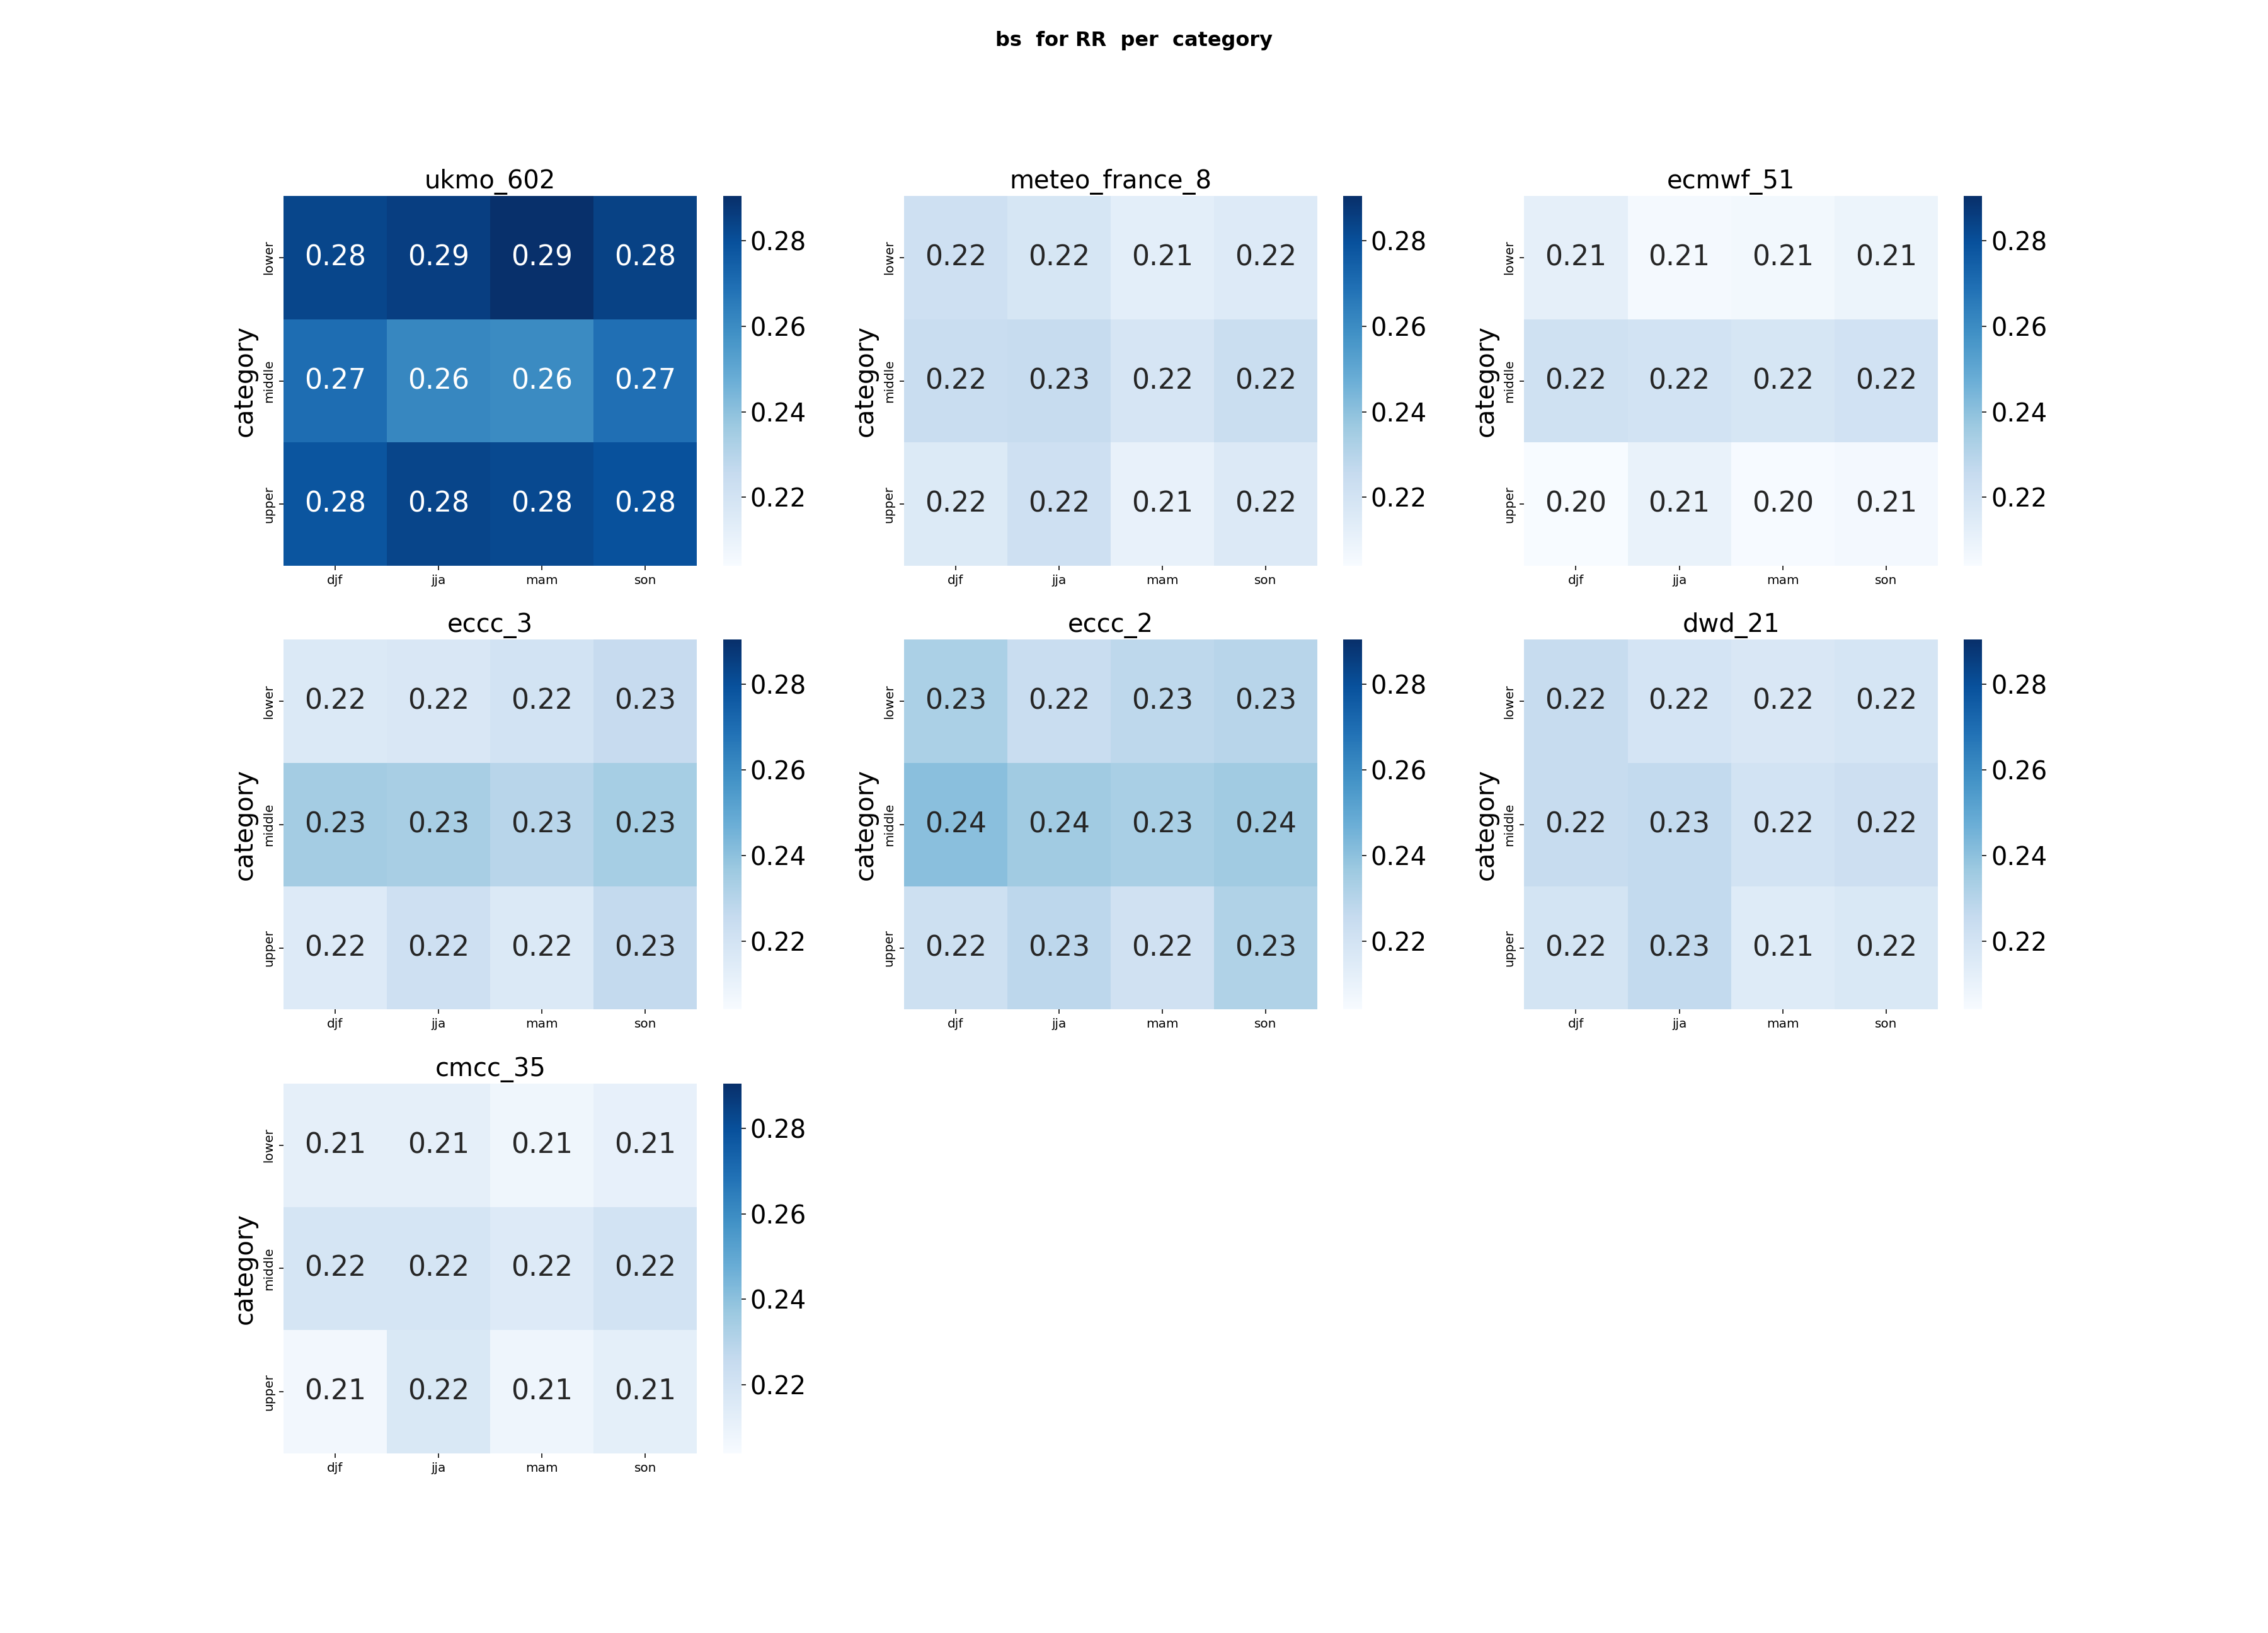
\includegraphics[scale=0.25]{plots/prob/bs/bs_RR_category.png}
    \caption{The Heatmap of Brier Score for each category  . \textbf{\textit{(0 represents perfect BS)}}}
\end{figure}

for the analysis per category, we can see in the figure above that all centers exhibit good performance in term of Brier Score except the UMKO that shows moderate BS. Overall, the middle tercile shows lower performance (higher Brier Score) for all centers. 
the figure below shows the analysis per lead-time. the same result is found, but the \textbf{\textit{ECMWF,METEO-FRANCE and CMCC-35}} are the best models in Brier Score for lead-time analysis.The performance stay stable along time which is a reliable signal. Despite the UKMO have the lower performance, it stays close to the other centers, the difference isn't so wide. 
In general, the performance stays stable over category, lead-time and space.


\begin{figure}[H]
    \centering
    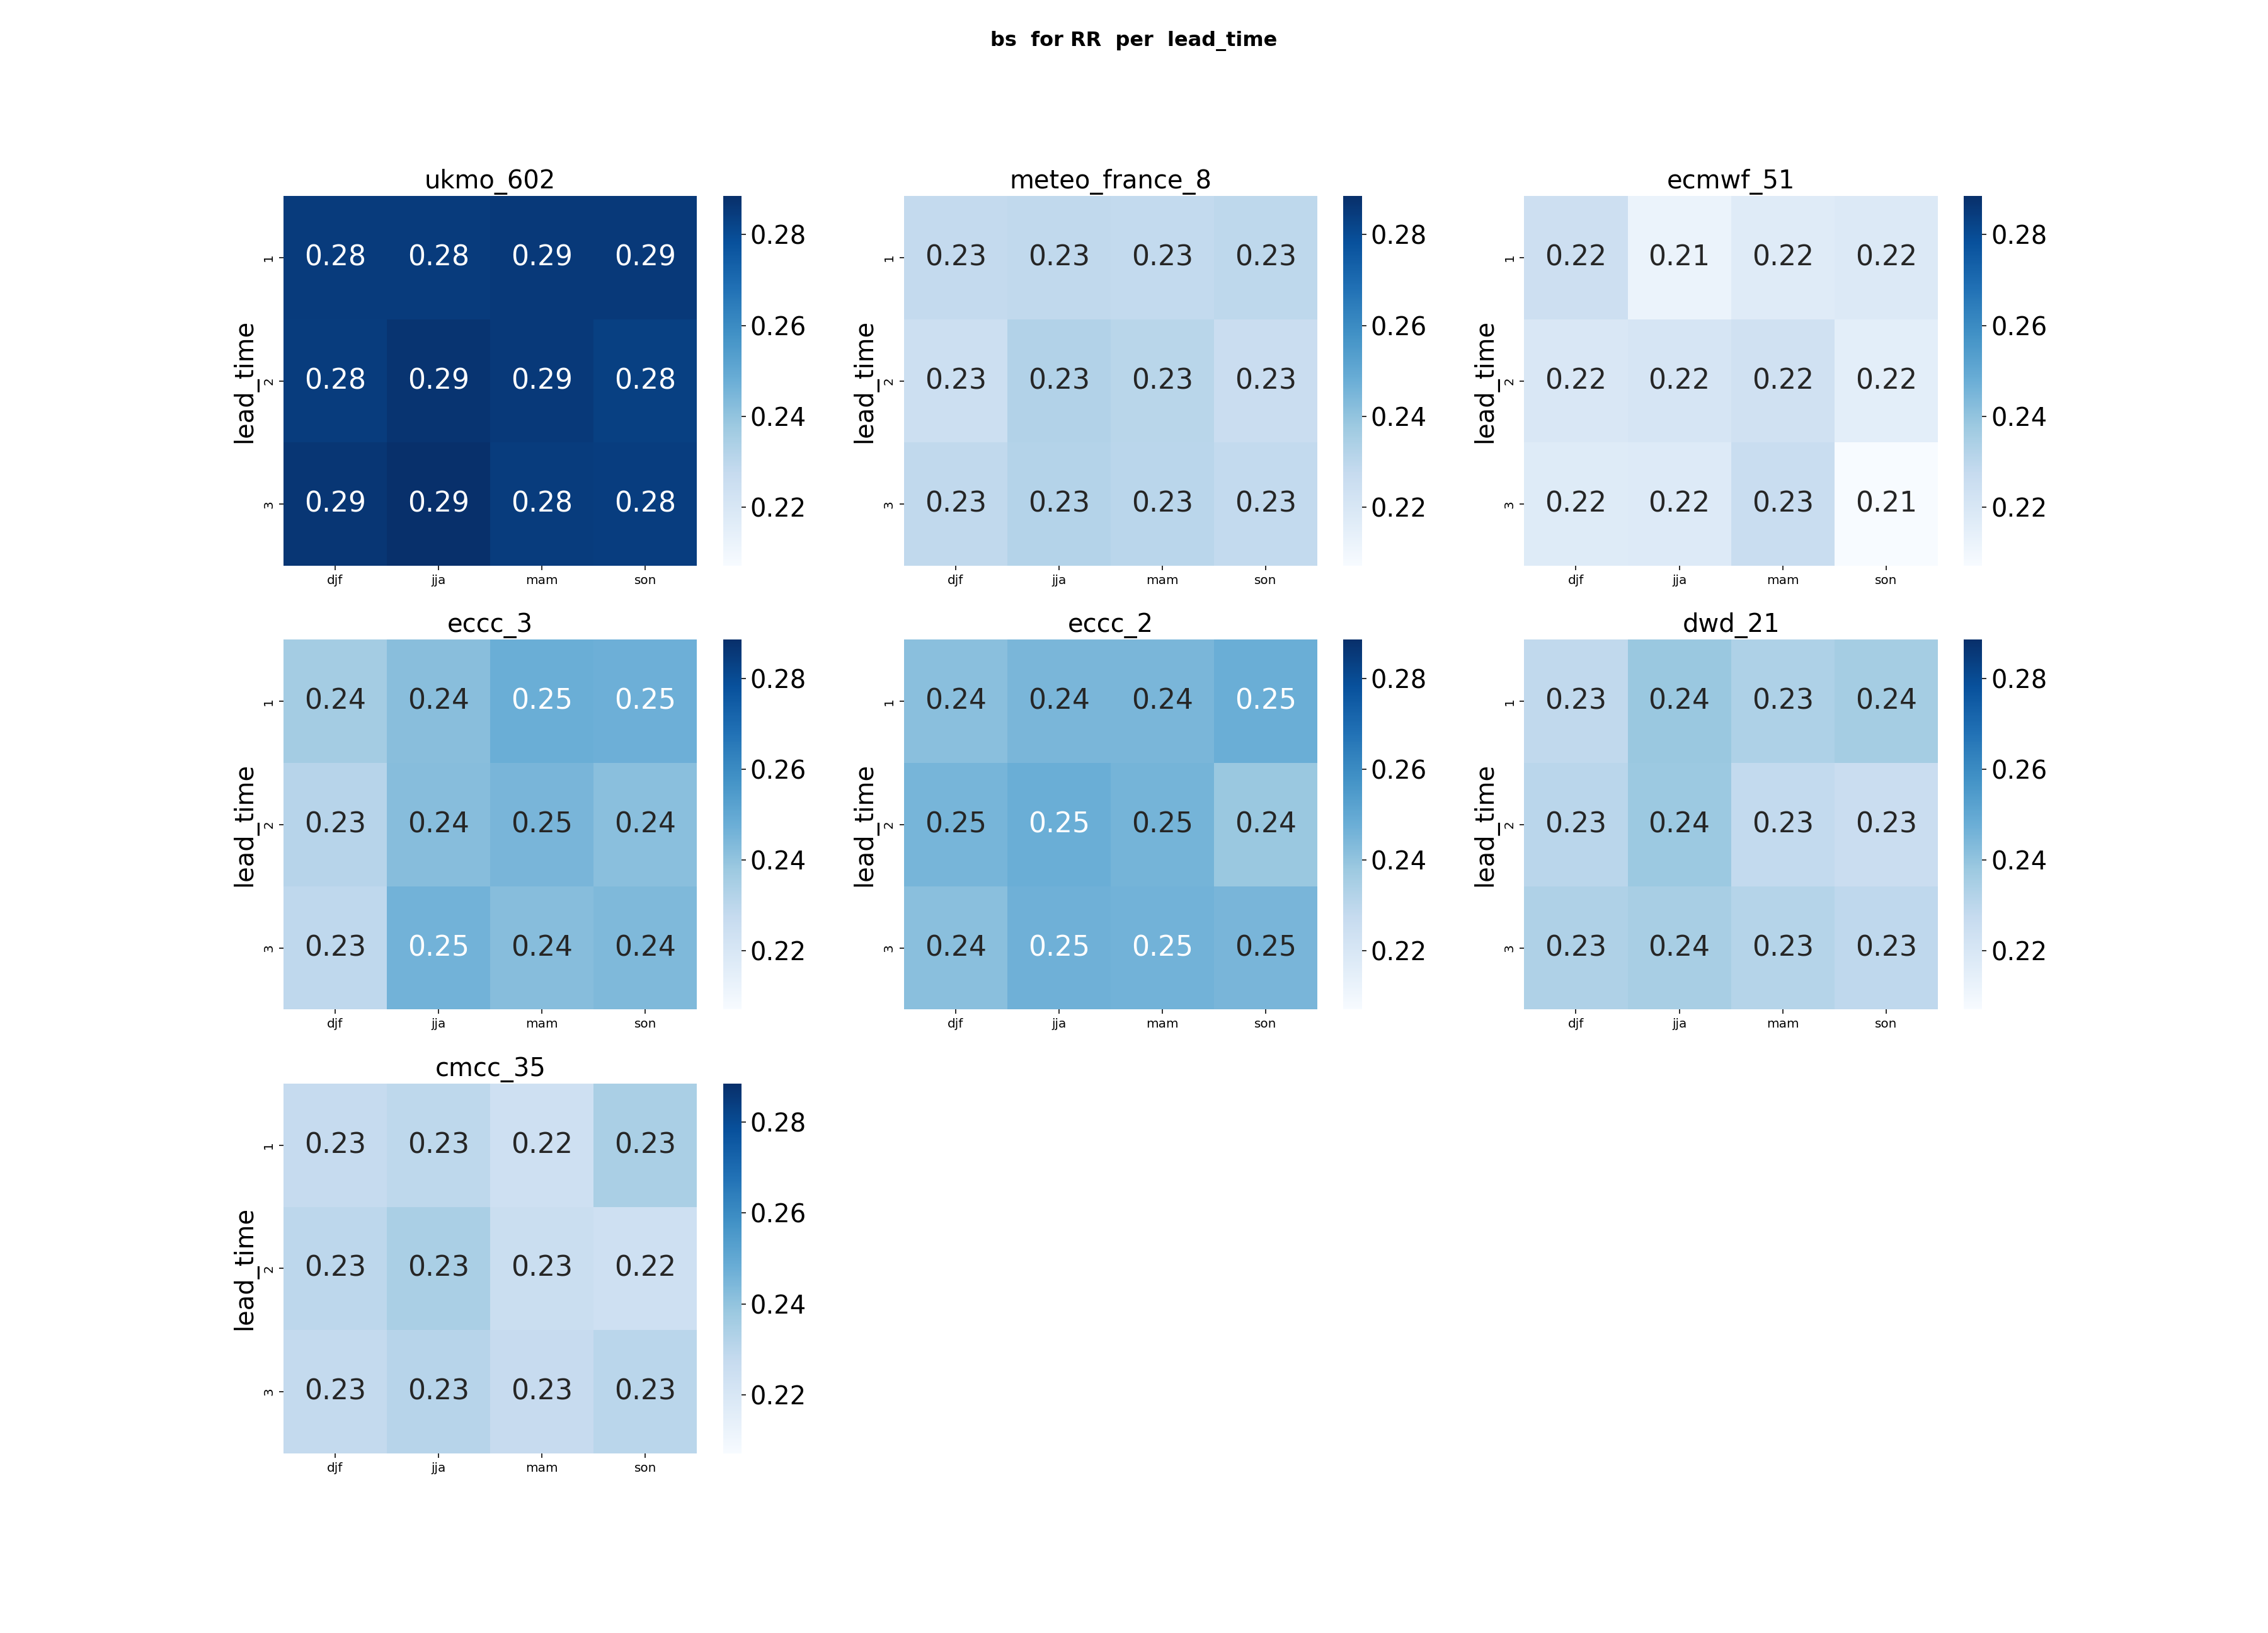
\includegraphics[scale=0.25]{plots/prob/bs/bs_RR_lead_time.png}
    \caption{The Heatmap of Brier Score for lead-time. \textbf{\textit{(0 represents perfect BS)}}}
\end{figure}


\begin{figure}[H]
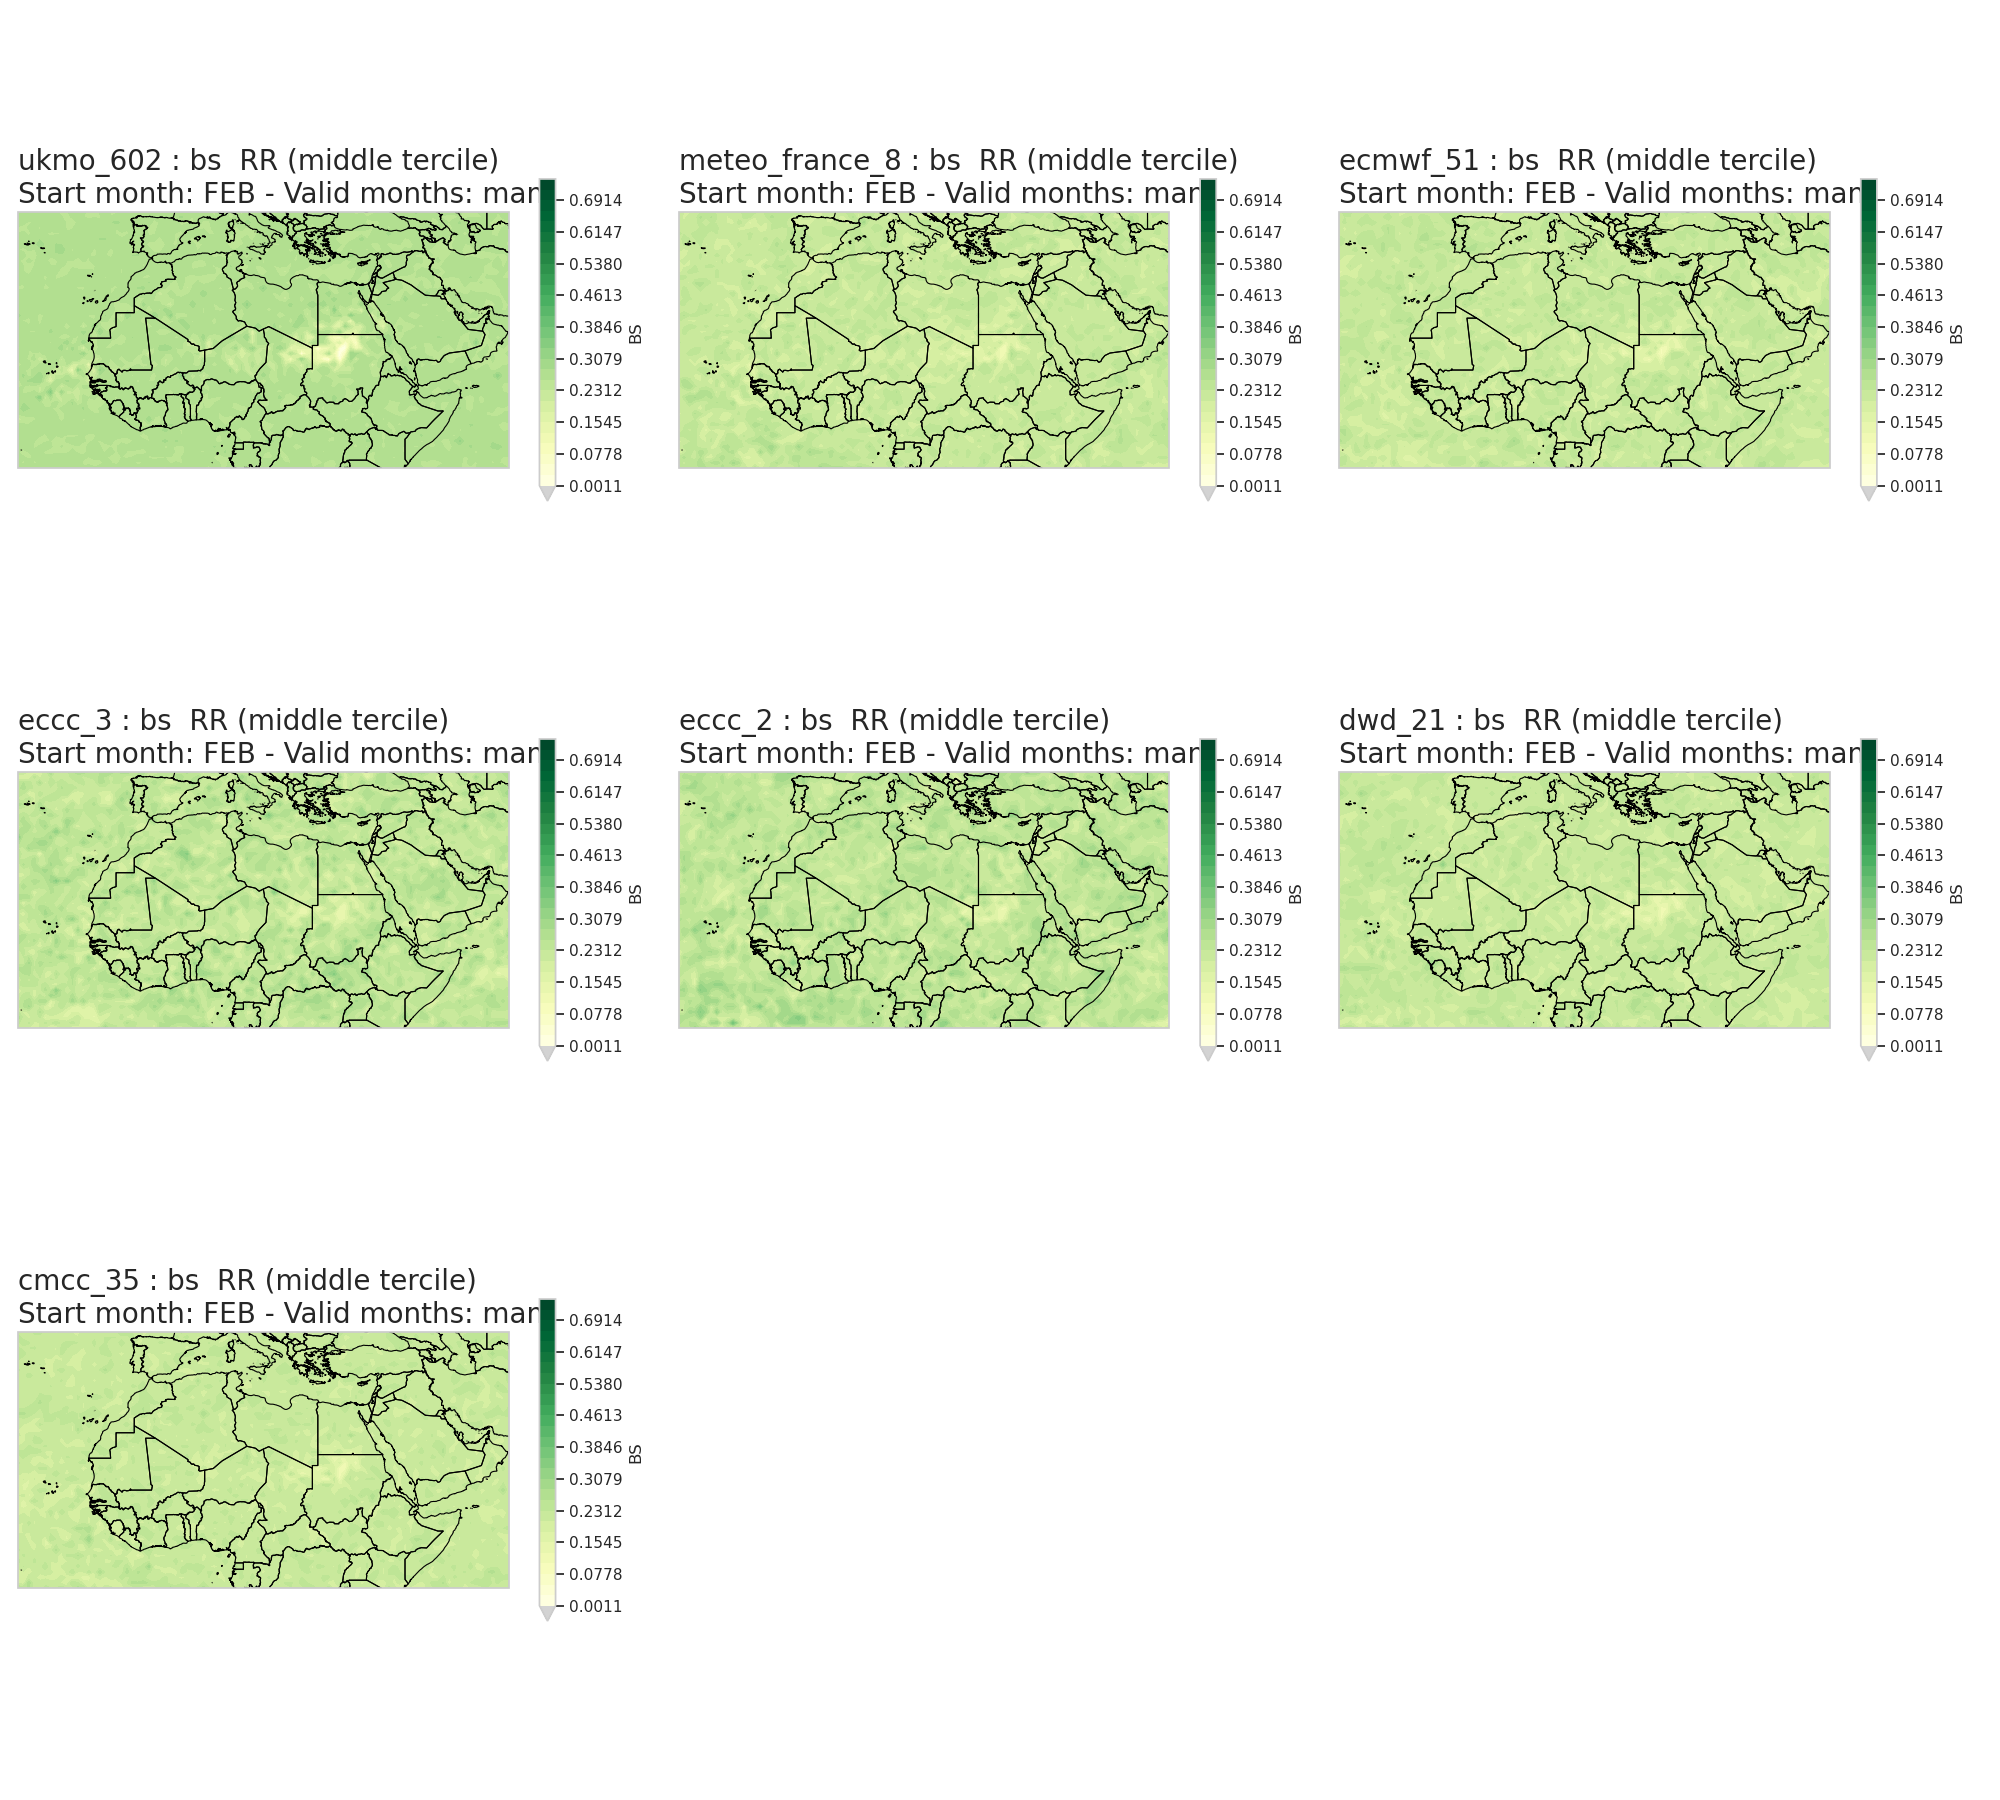
\includegraphics[scale=0.3]{plots/prob/bs/bs_mam_RR_middle.png}
\caption{3-months Rolling mean of Brier Score in MENA Region for all centers middle tercile MAM}
\end{figure}

the spacial distribution of the BS is homogeneous, the same performance across the MENA region, almost all centers perform well for all lead-times, for  tercile there is a little lower performance for the middle tercile.
Hint, for the other seasons the results are almost the same. 


\subsubsection{Reliability}

\begin{figure}[H]
    \centering
    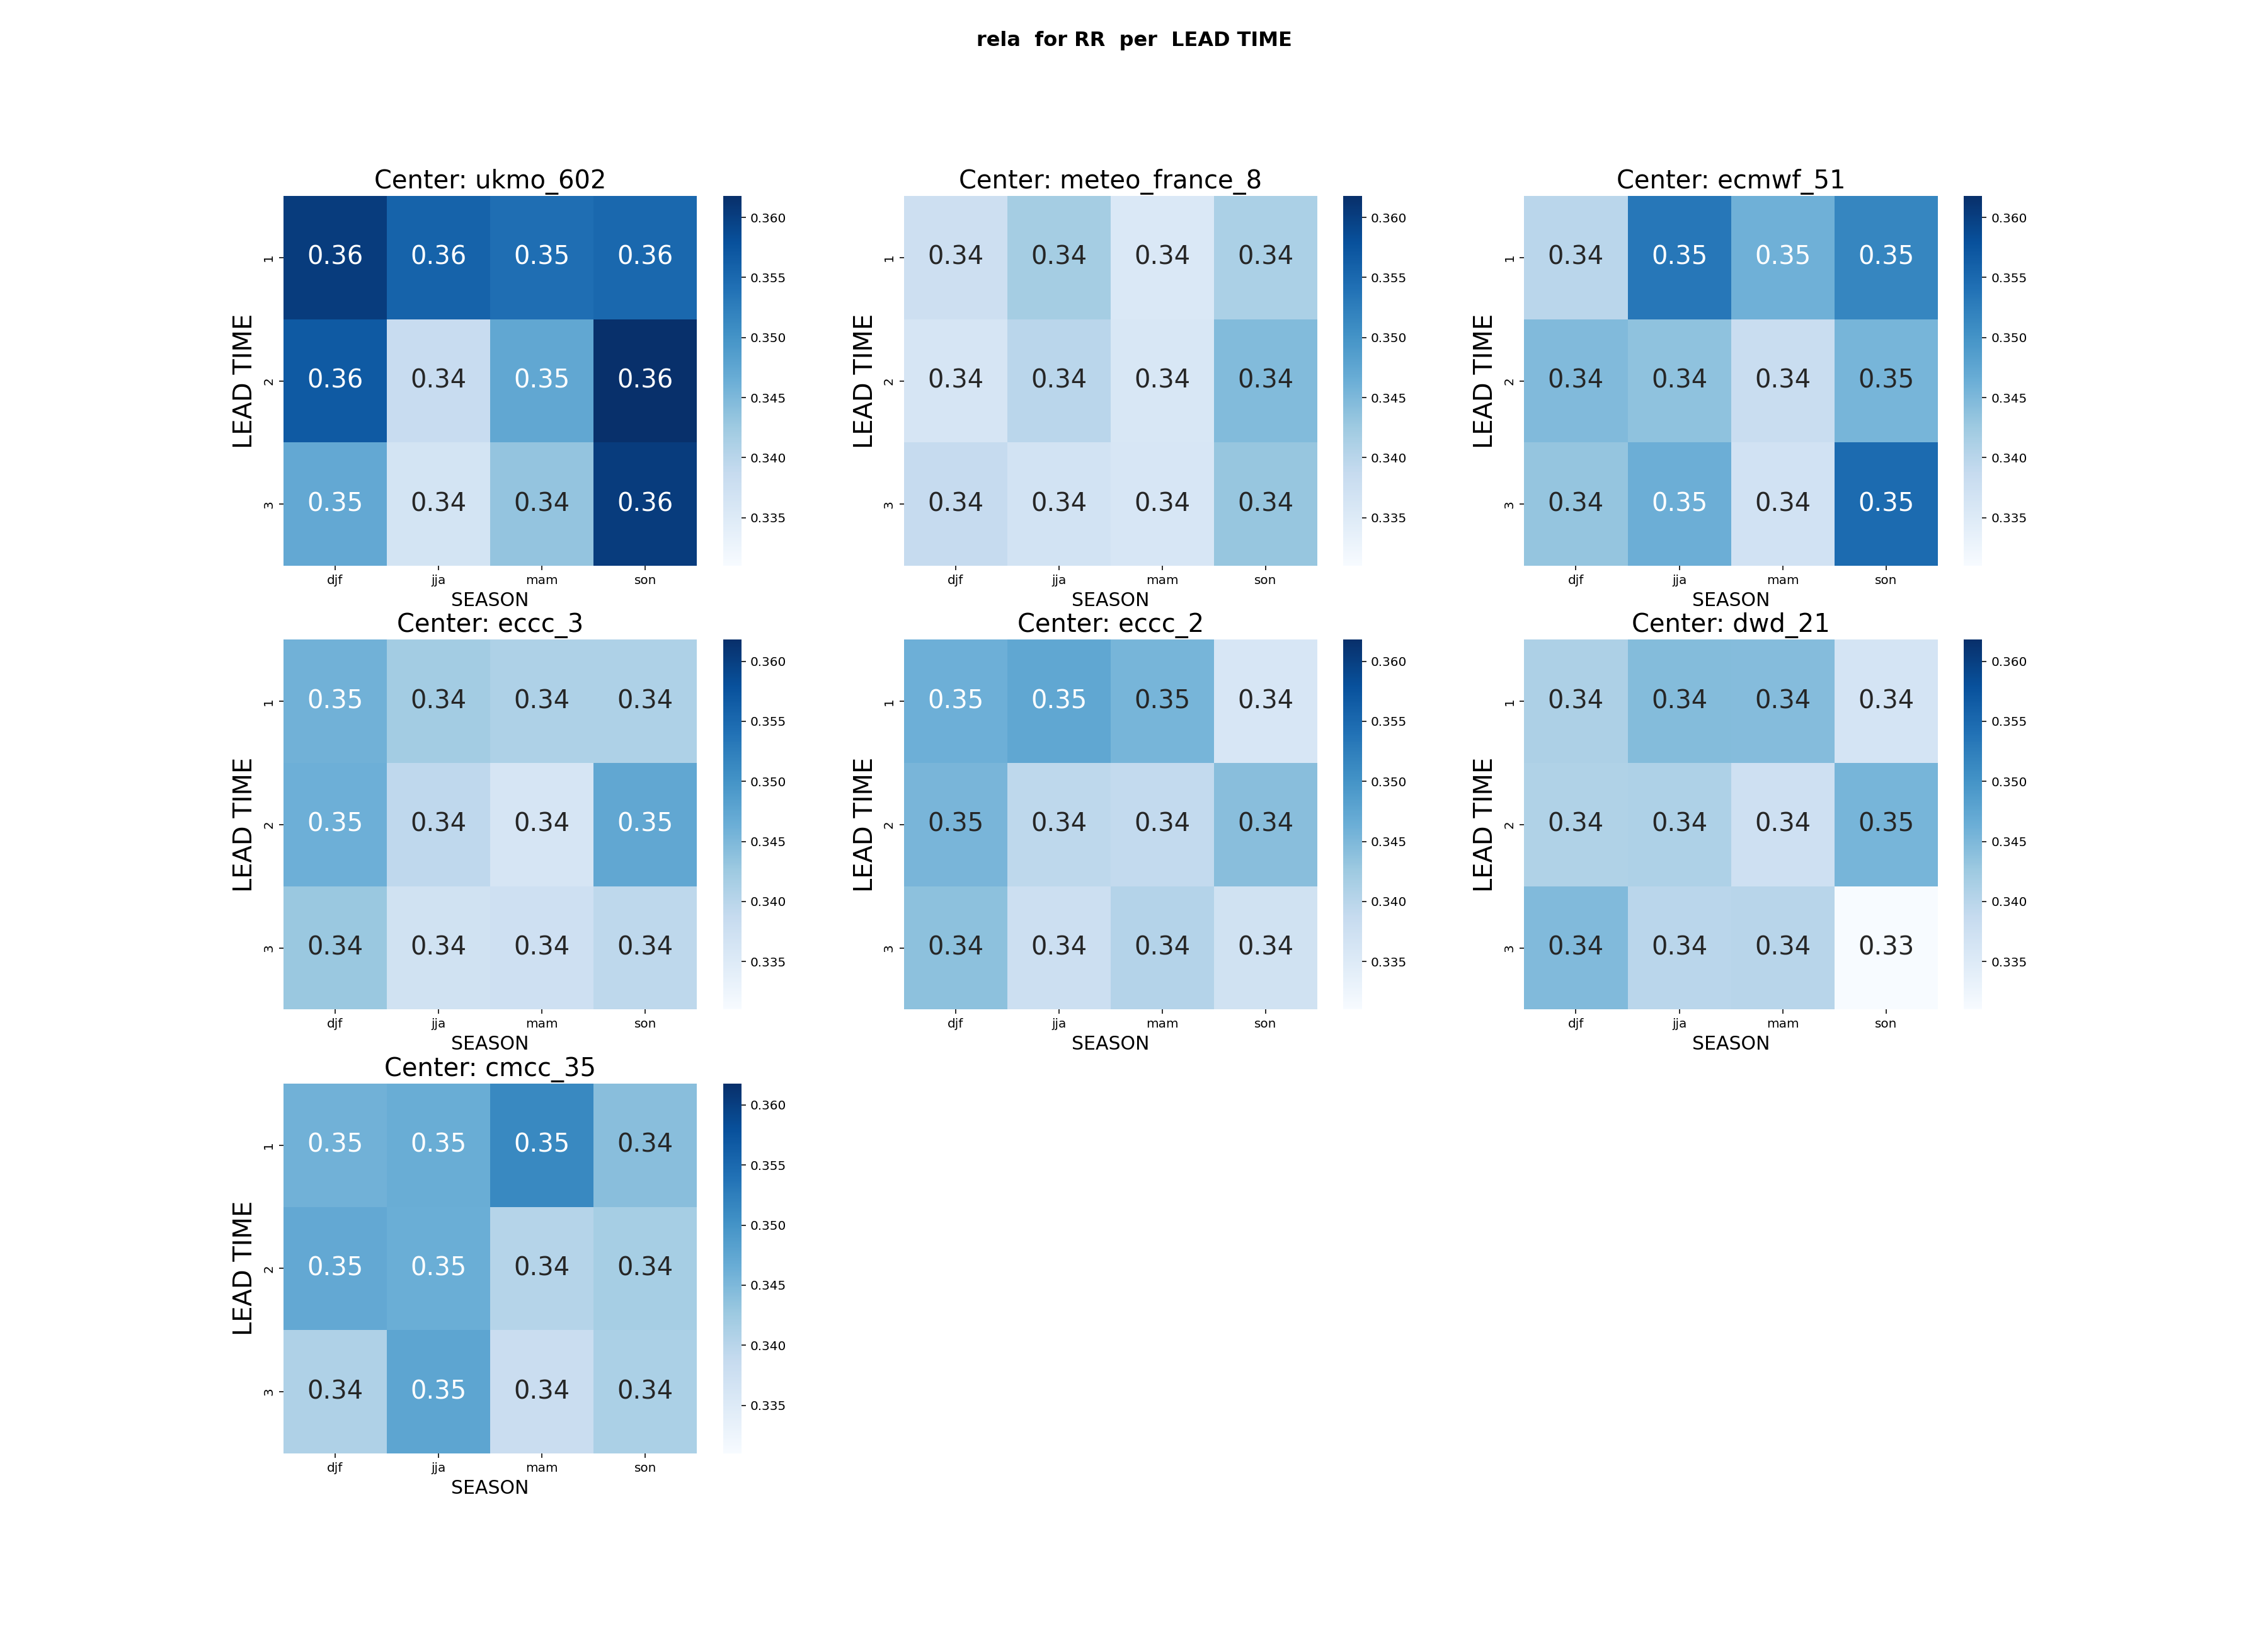
\includegraphics[scale=0.25]{plots/prob/rela/rela_RR.png}
    \caption{The Reliability Score  . \textbf{\textit{(0 means perfect Reliability)}}}
\end{figure}

In the figure above, all centers demonstrate similar moderate performance in term of reliability. But deep analysis within the figure below, shows that UKMO has very bad performance, also we can distinguish three models that have the best reliability according to the reliability diagram, the centers are \textbf{\textit{ECMWF,CMCC and METEO-FRANCE}}. Hence,all centers give similar description of the reliability, also the stability along lead-time is a good indicator despite of the moderate results (0.3), we can rely on the models cited above because of the acceptable results and the stability along time.

\begin{figure}[H]
\centering
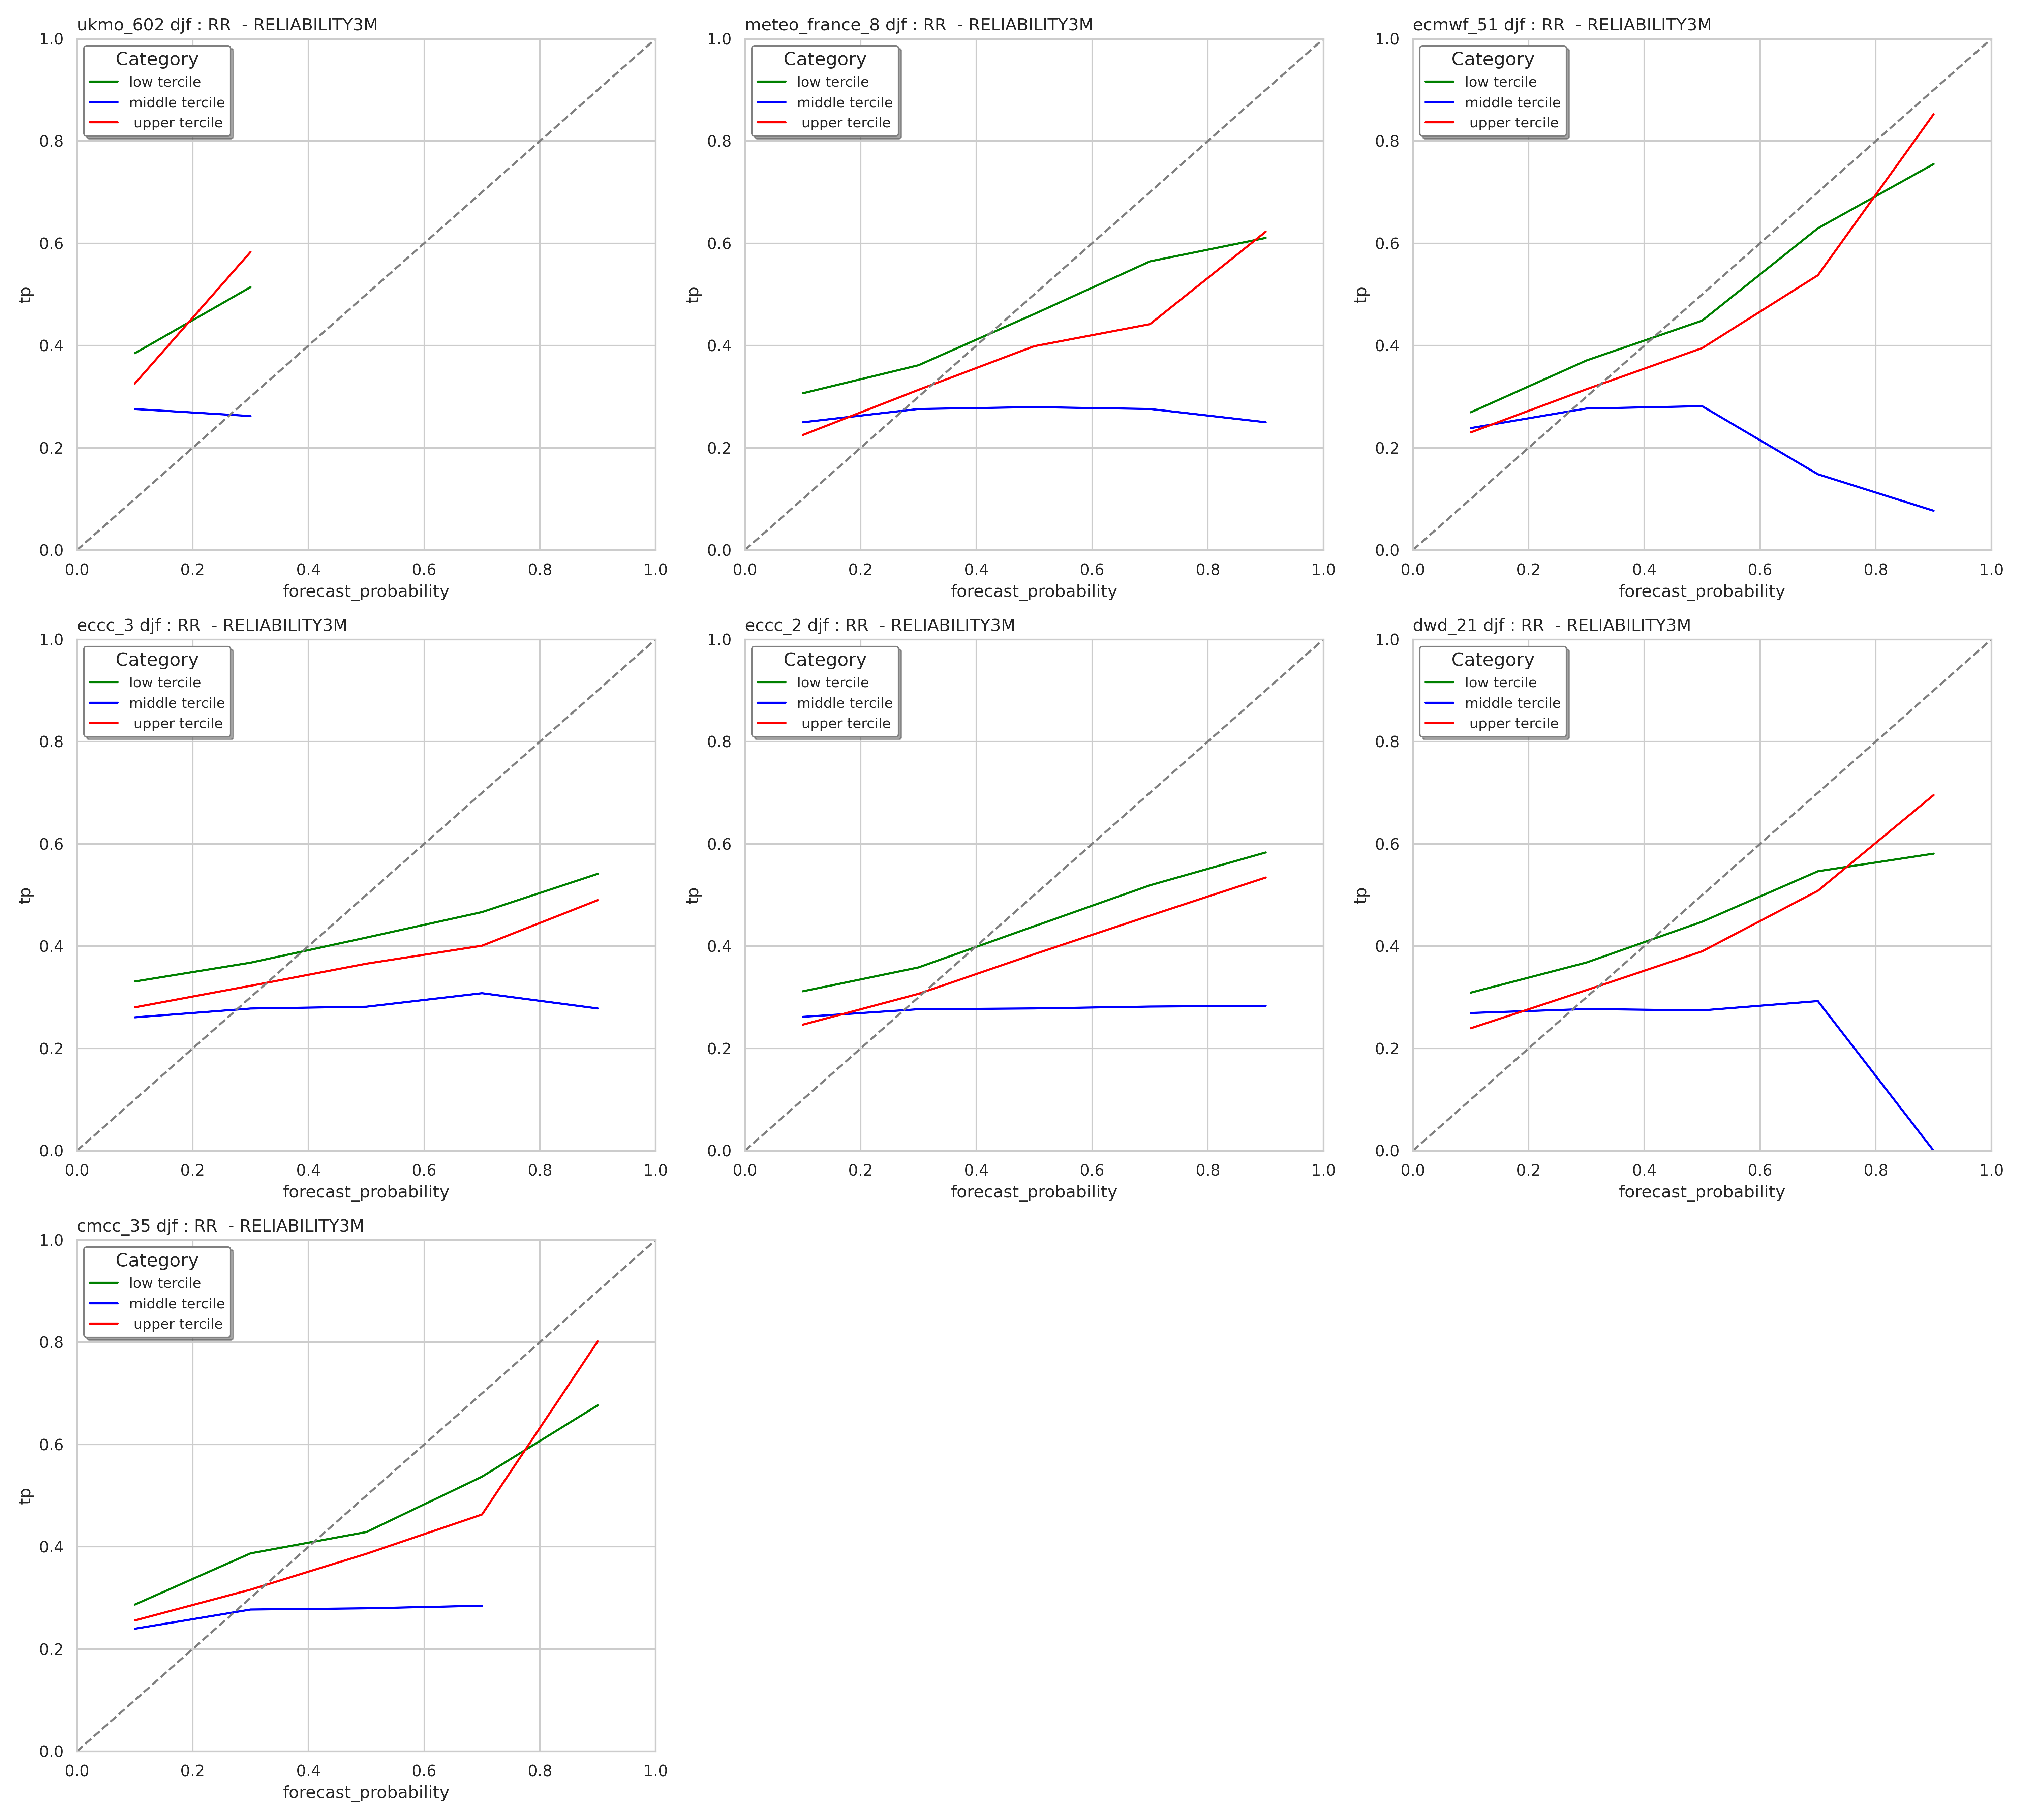
\includegraphics[scale=0.3]{plots/prob/rela/rela_diagram_RR_djf.png}
\caption{The 3-month rolling mean for Reliability DJF   . \textbf{\textit{Reliability is better in cases where the graphs are closer to the 45-degree line}}}
\end{figure}

for the reliability diagram, all centers show moderate results, except for the ukmo that shows lower reliability.Thus, for the lower and upper terciles, models in general show good reliability, but for the middle tercile, this models aren't reliable. above all, \textbf{\textit{ecmwf}}  shows the highest performance for reliability.


\subsubsection{The ranked probability score (RPS)}


\begin{figure}[H]
    \centering
    \includegraphics[scale=0.25]{plots/prob/rps/rps_RR.png}
    \caption{The Heatmap of  RPS Score on MENA region for Precipitations    . \textbf{\textit{(0 means perfect RPS)}}}
\end{figure}

In the figure above, all centers demonstrate moderate performance, except for UKMO, which shows noticeably lower performance. 


\begin{figure}[H]
    \centering
    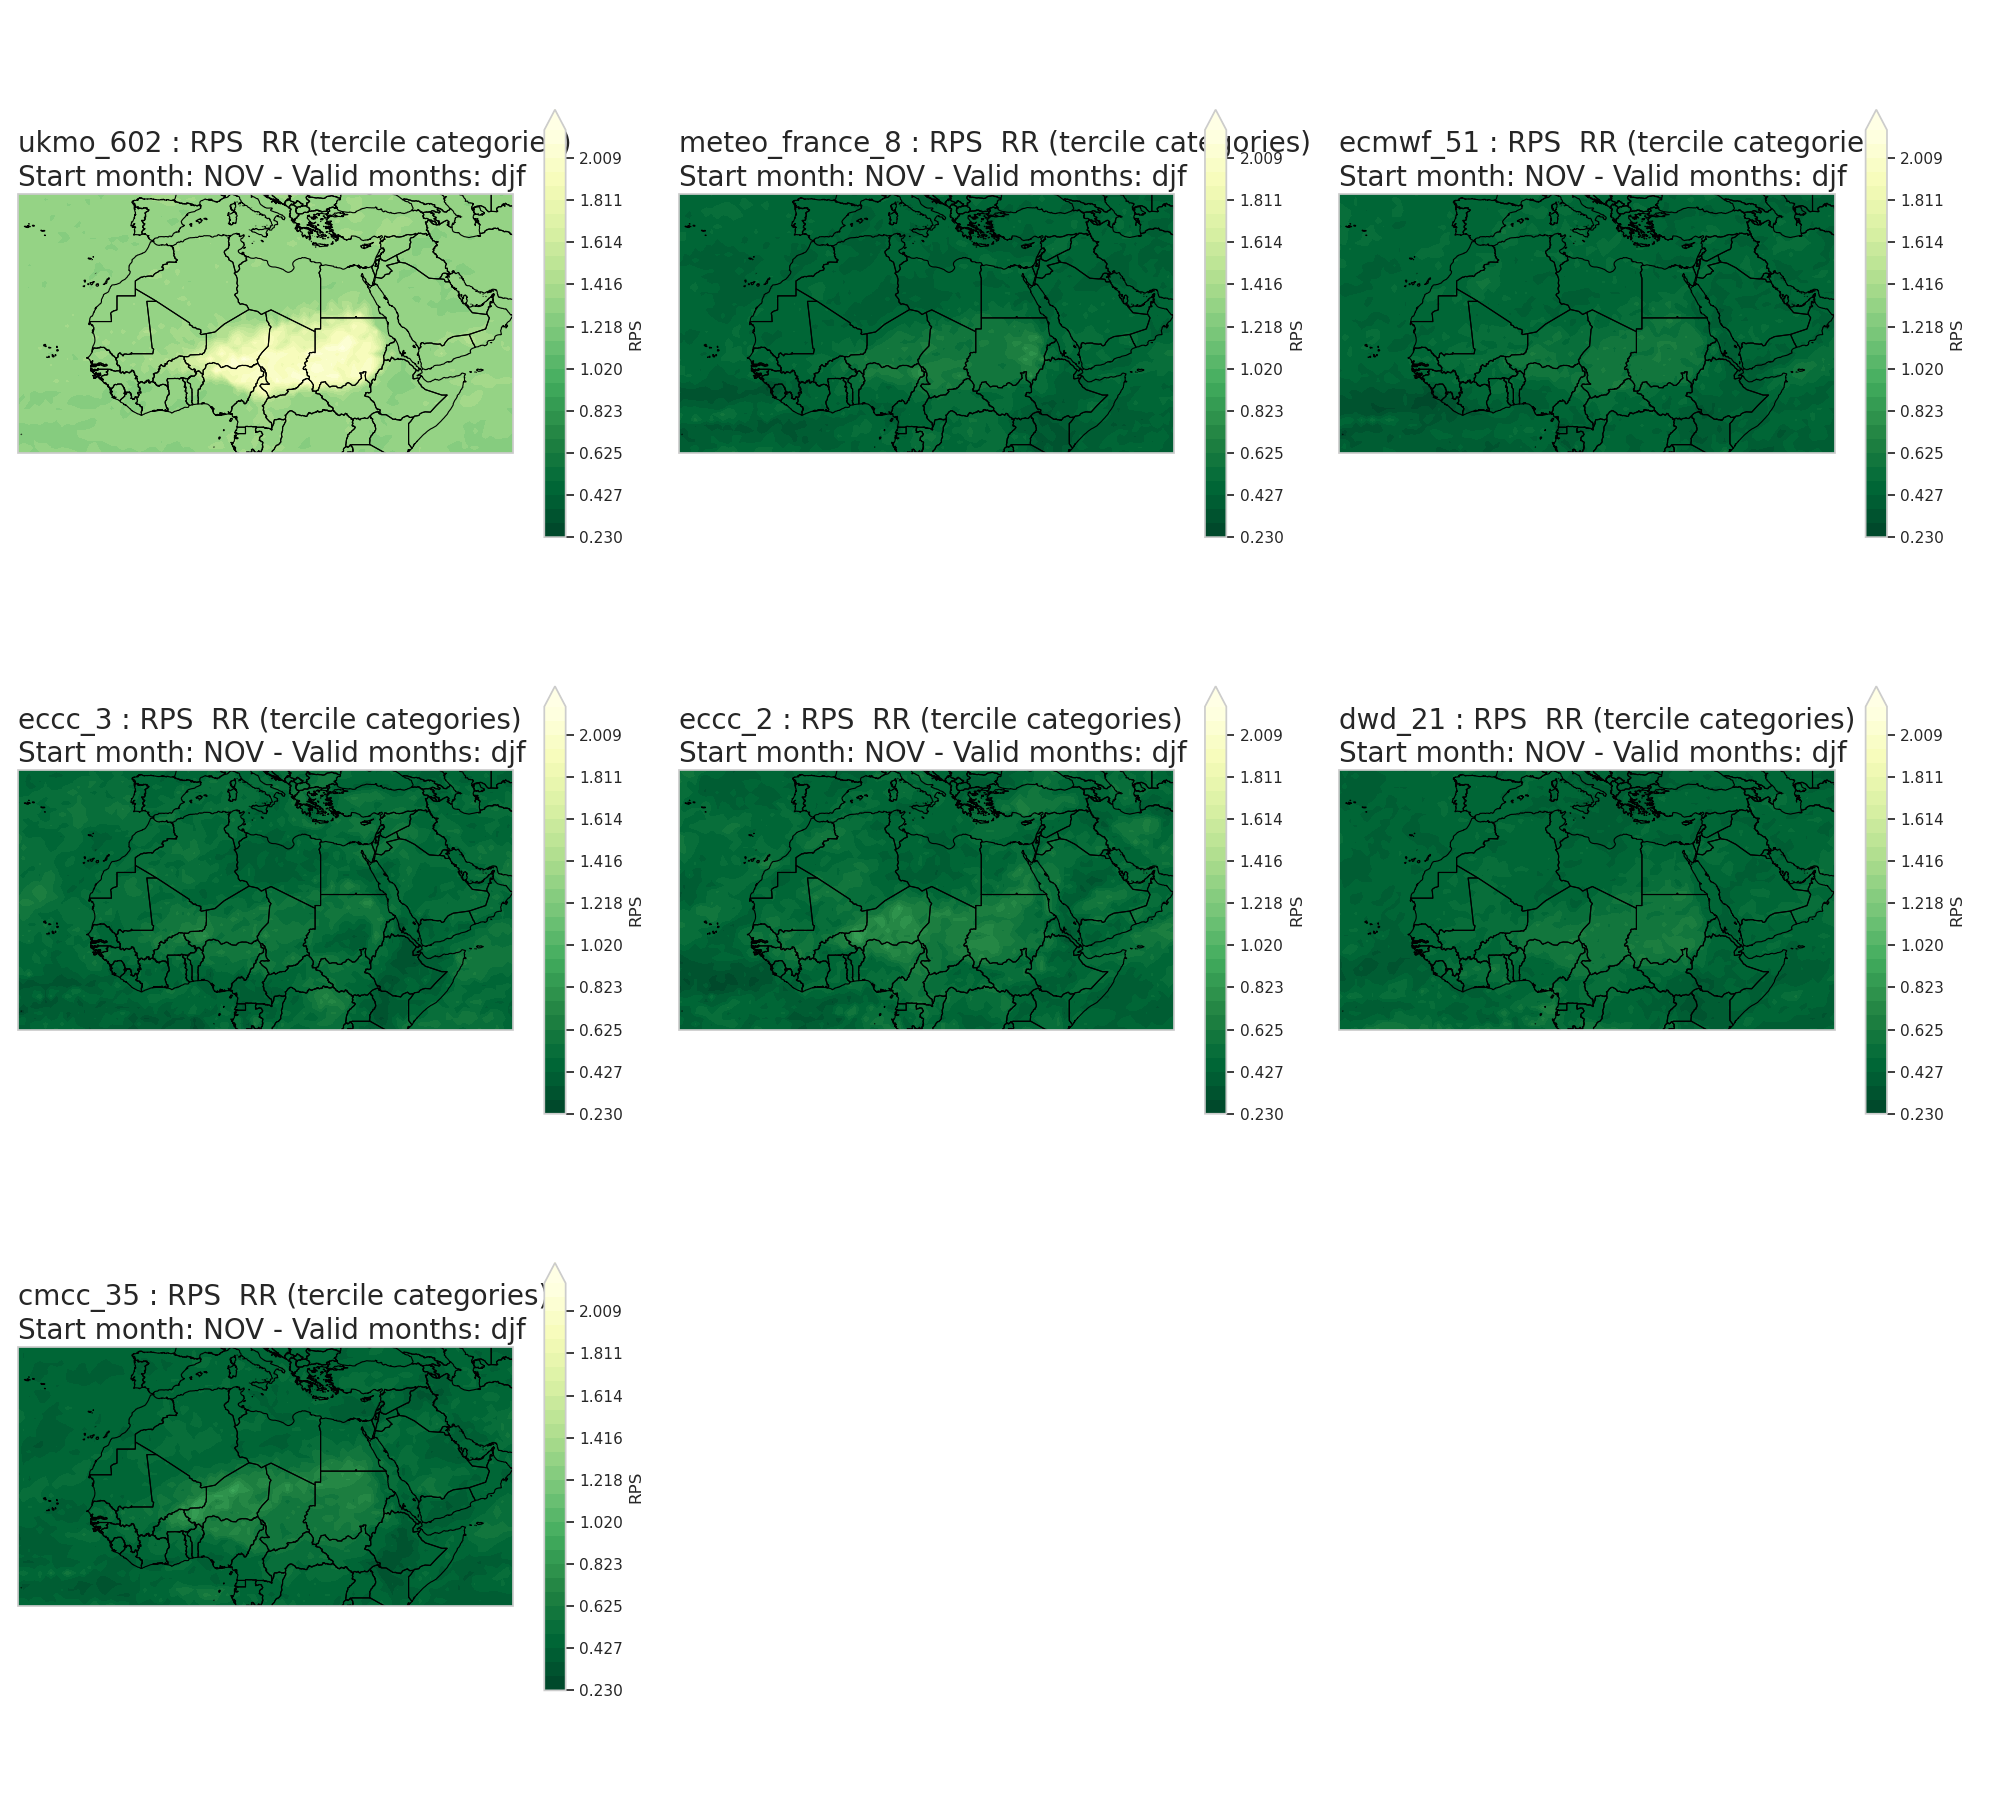
\includegraphics[scale=0.25]{plots/prob/rps/rps_djf_RR.png}
    \caption{The   RPS Score on MENA region for Precipitations DJF   . \textbf{\textit{(0 means perfect RPS)}}}
\end{figure}

the spacial distribution of the RPS, is homogeneous, in all the region the score is good for all centers.Thus, the ukmo shows lower performance for this score.


\subsubsection{Relative operating characteristics}

\begin{figure}[H]
    \centering
    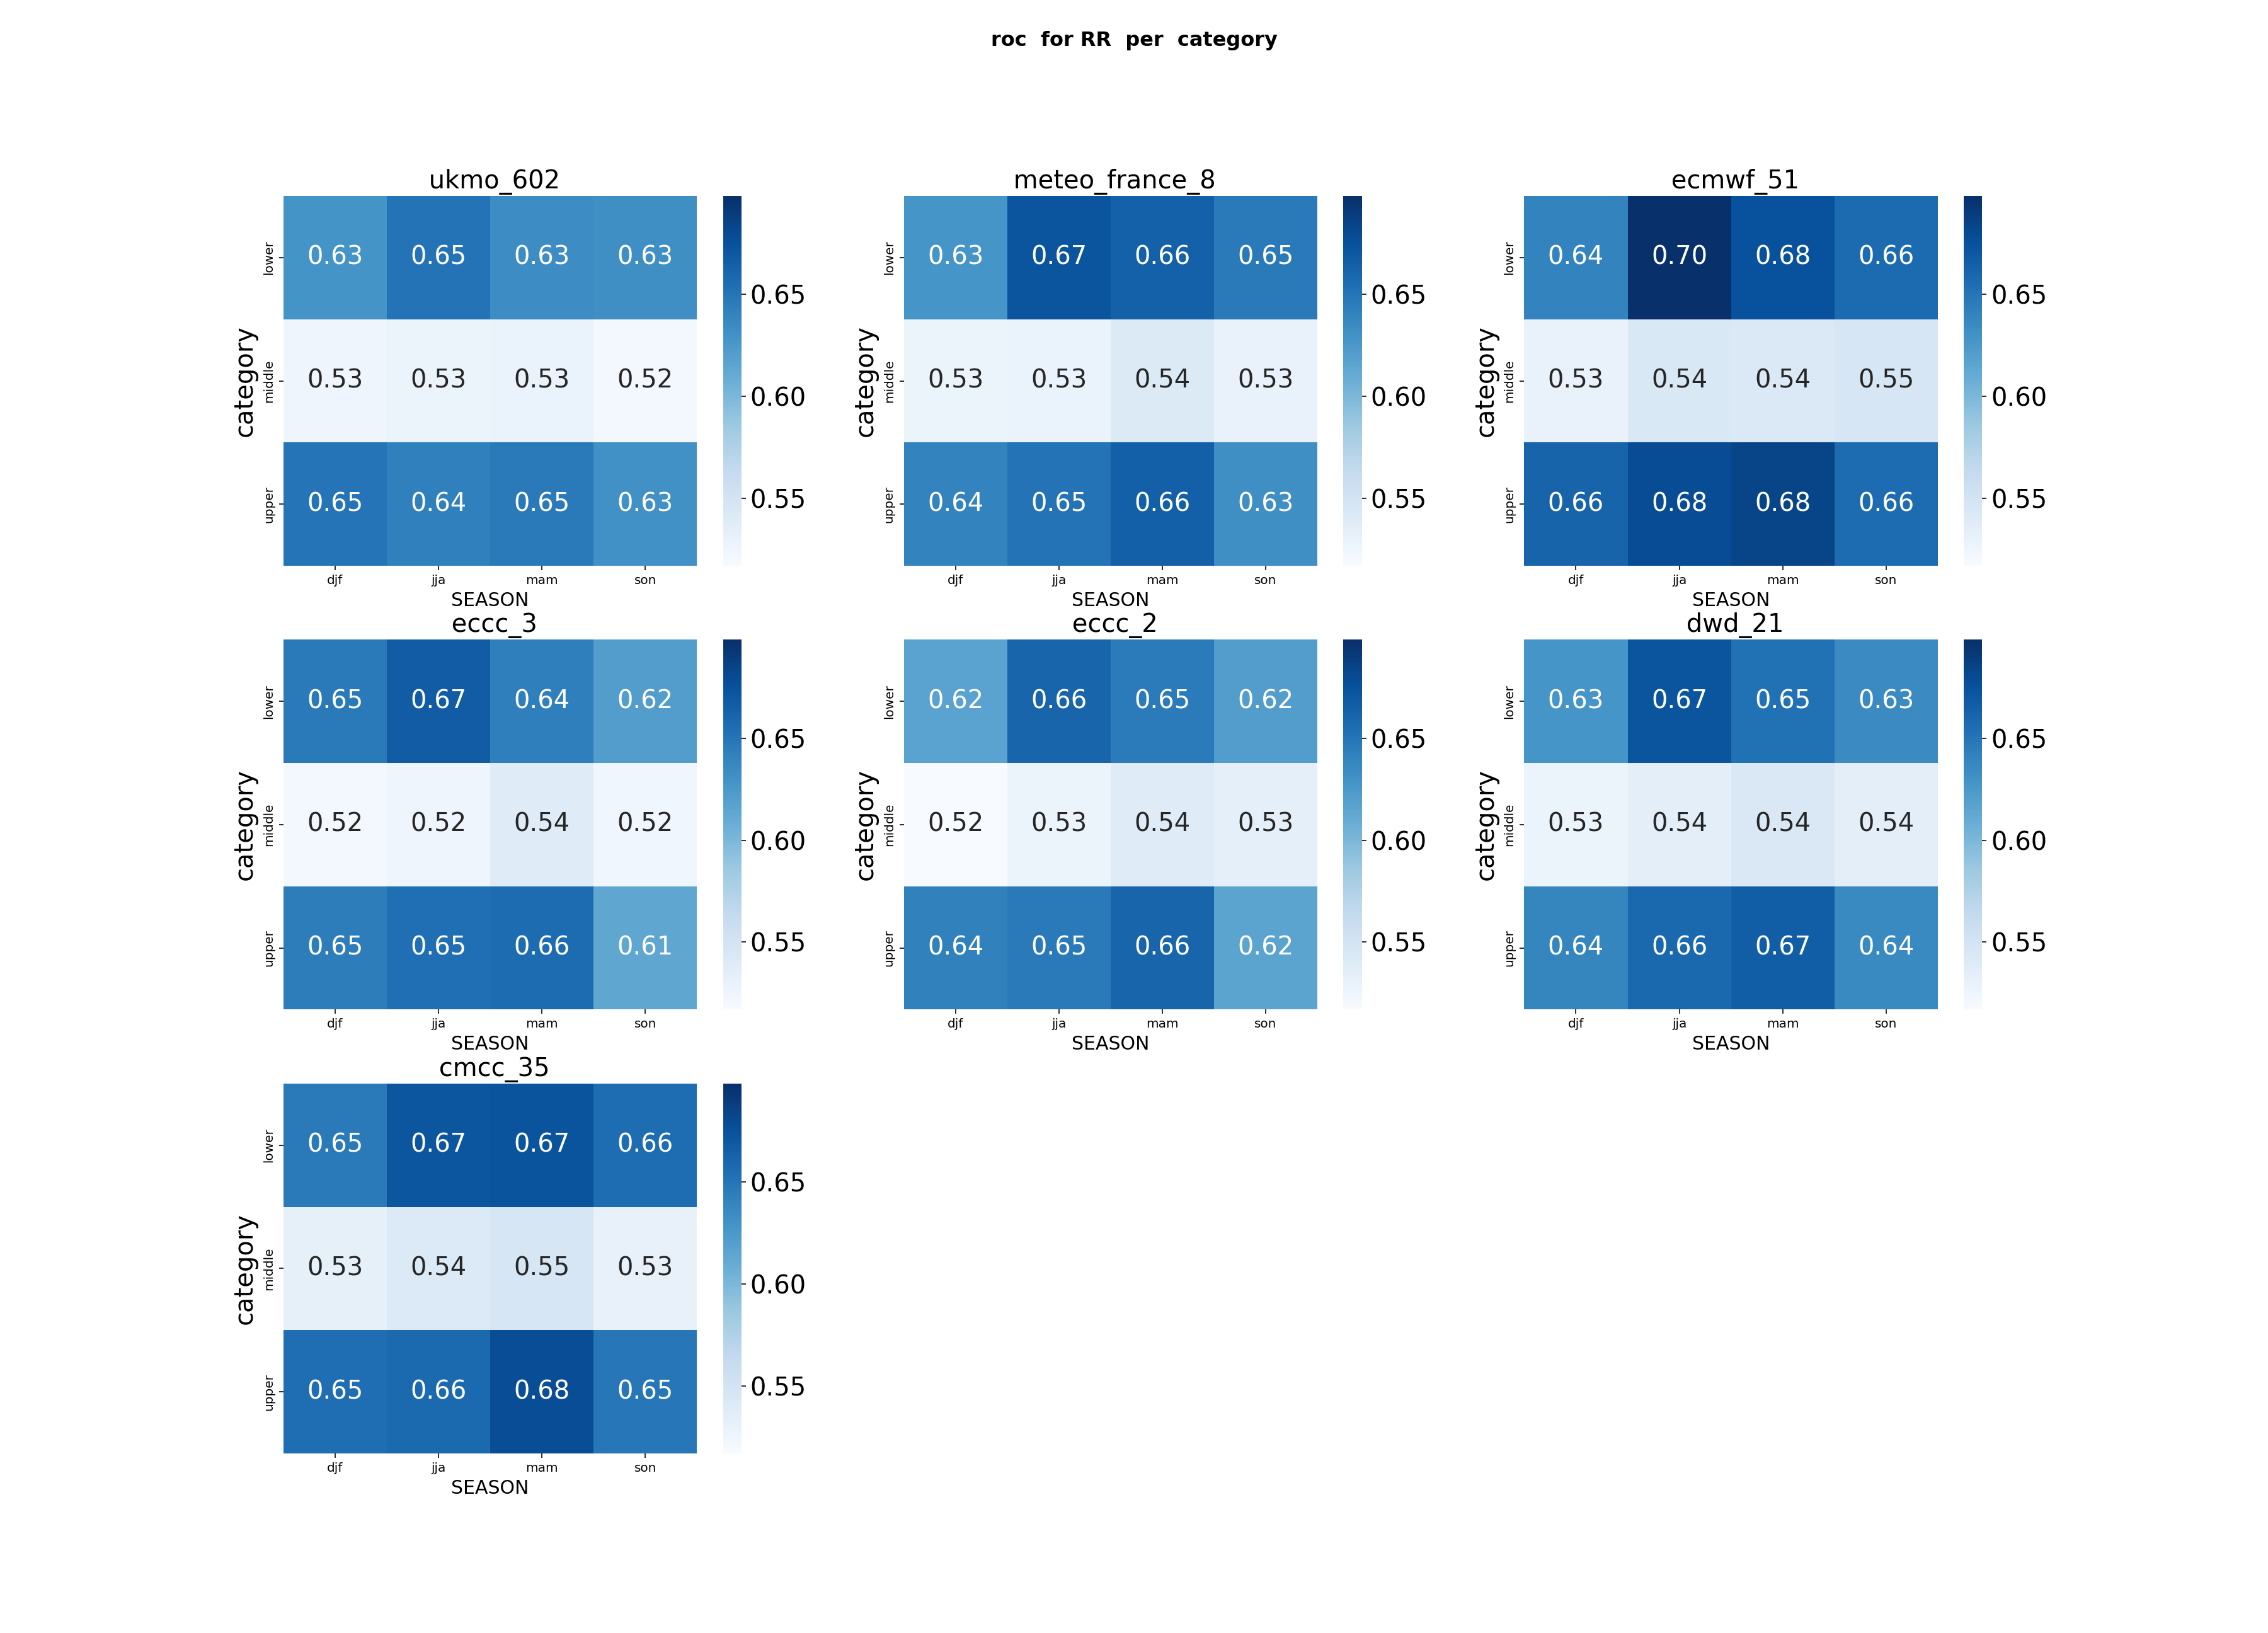
\includegraphics[scale=0.25]{plots/prob/roc/roc_RR_category.png}
    \caption{The Heatmap of ROC Score for each category  . \textbf{\textit{(1 means perfect ROC)}}}
\end{figure}

In the figure above, it is evident that all centers exhibit similar performance levels. However, the middle tercile consistently achieves the lowest score.
\begin{figure}[H]
    \centering
    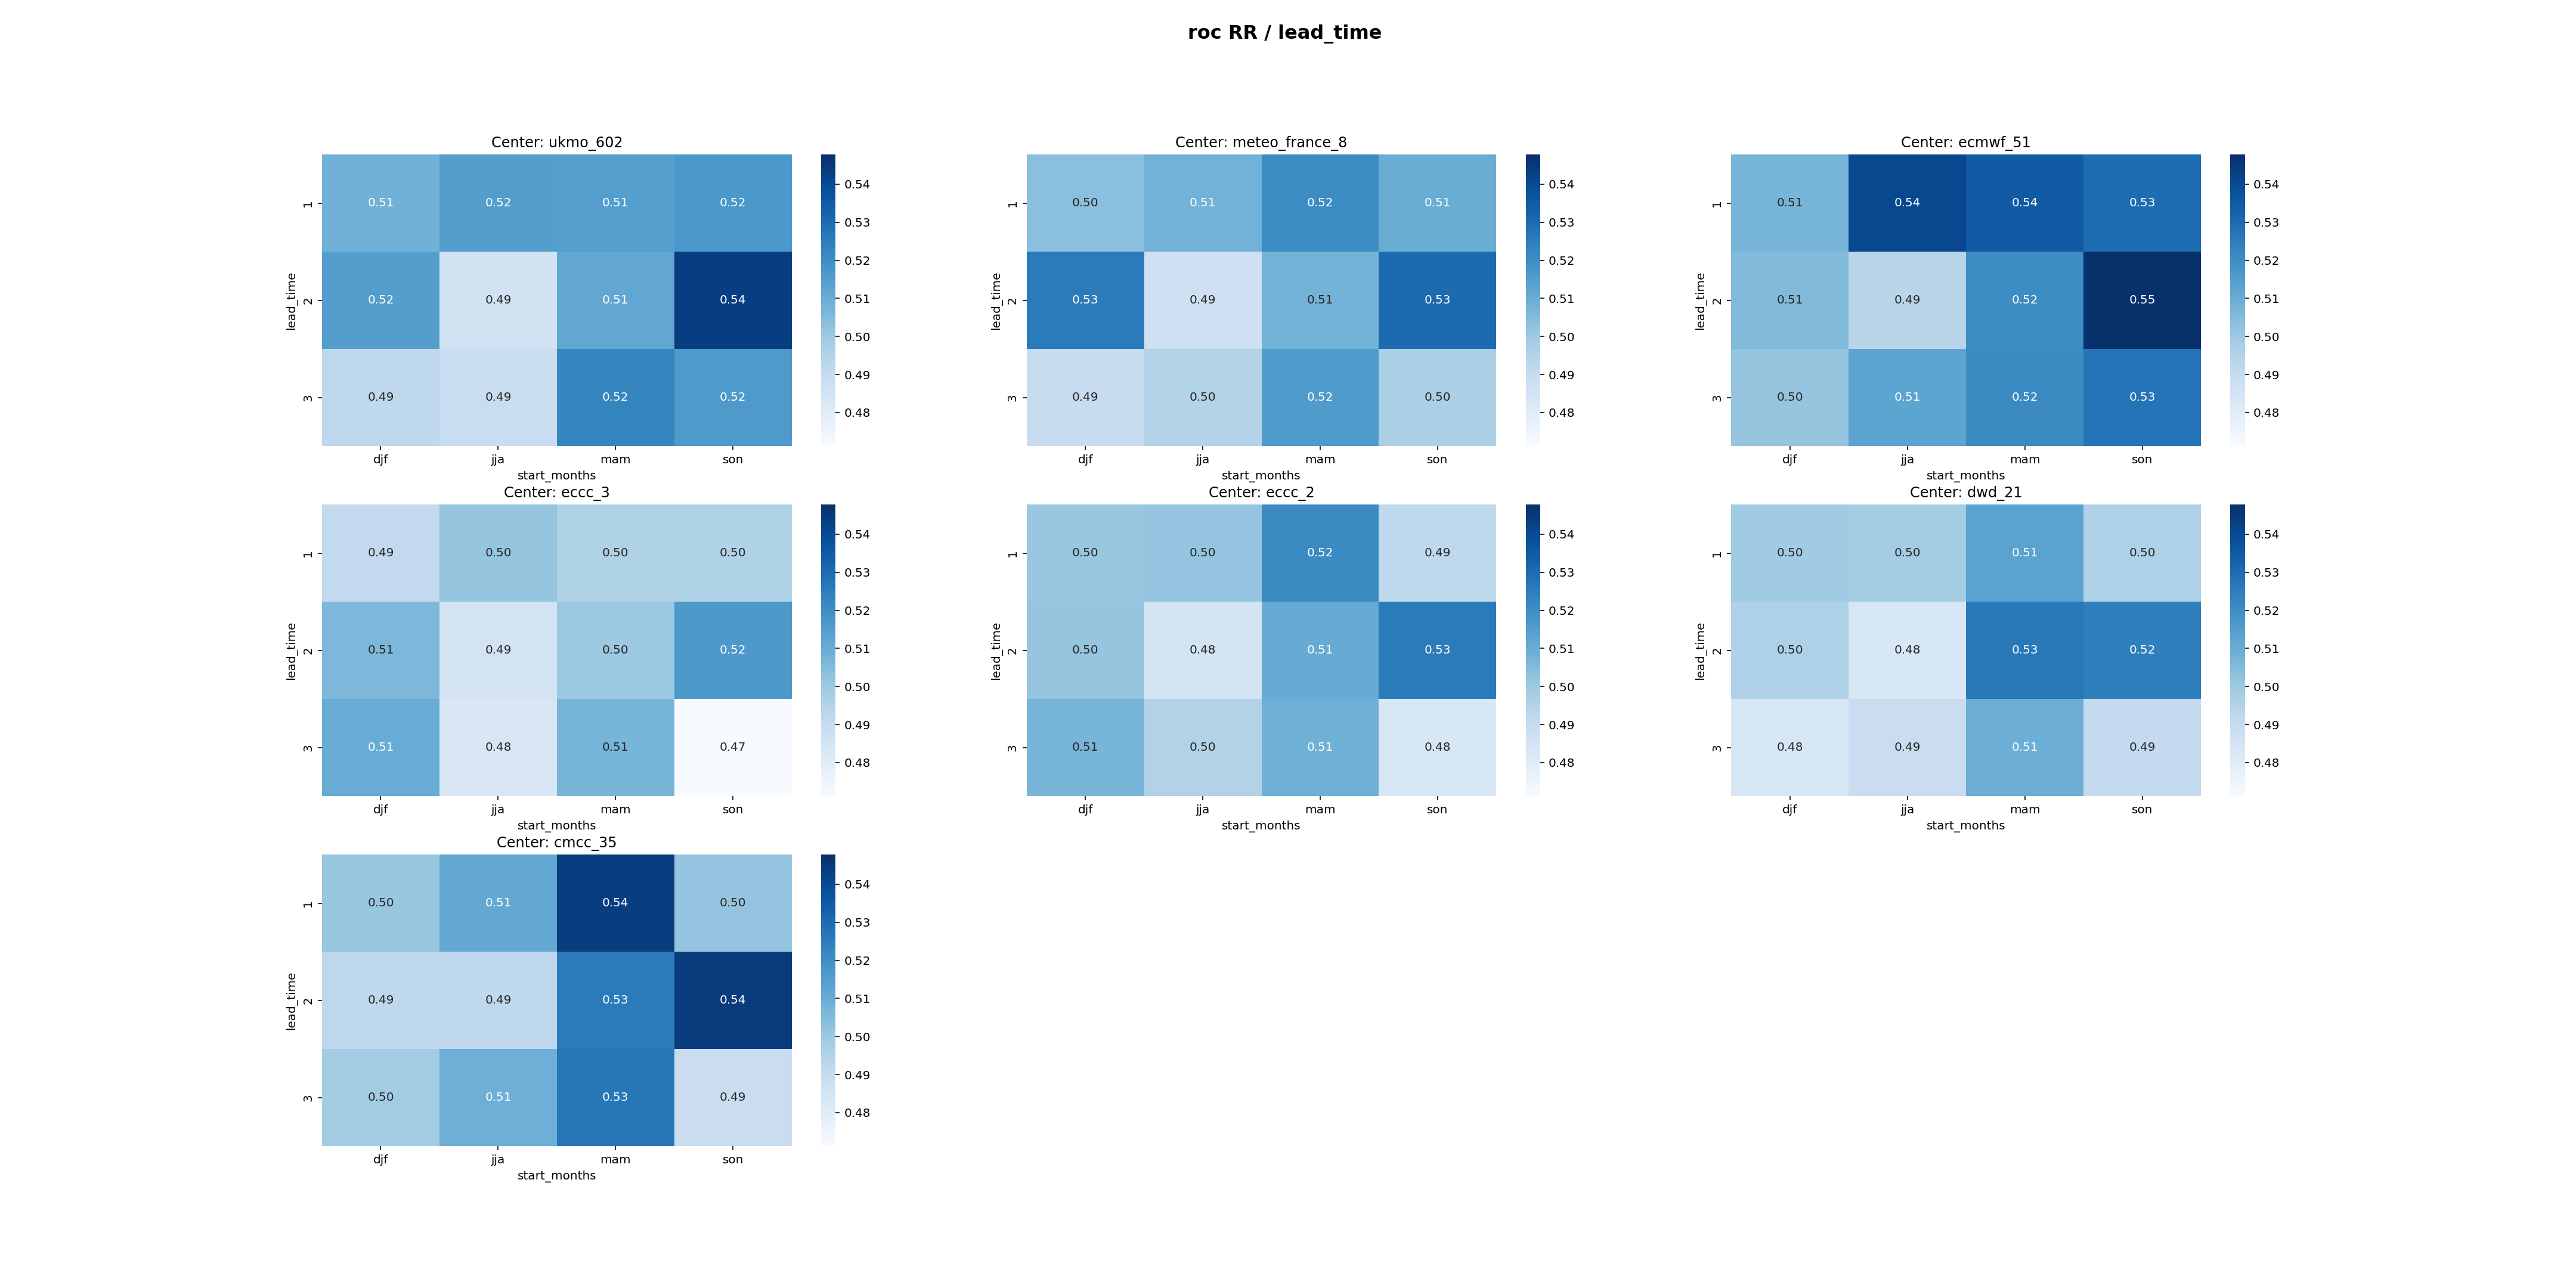
\includegraphics[scale=0.25]{plots/prob/roc/roc_RR_lead_time.png}
    \caption{The Heatmap of ROC Score for lead-times. \textbf{\textit{(1 means perfect ROC)}}}
\end{figure}

for the ROC score, all centers show similar good performance, in general the best score is observed for tha first lead-time, except for the SON season where the best performance is for the second lead-time.

\begin{figure}[H]
    \centering
    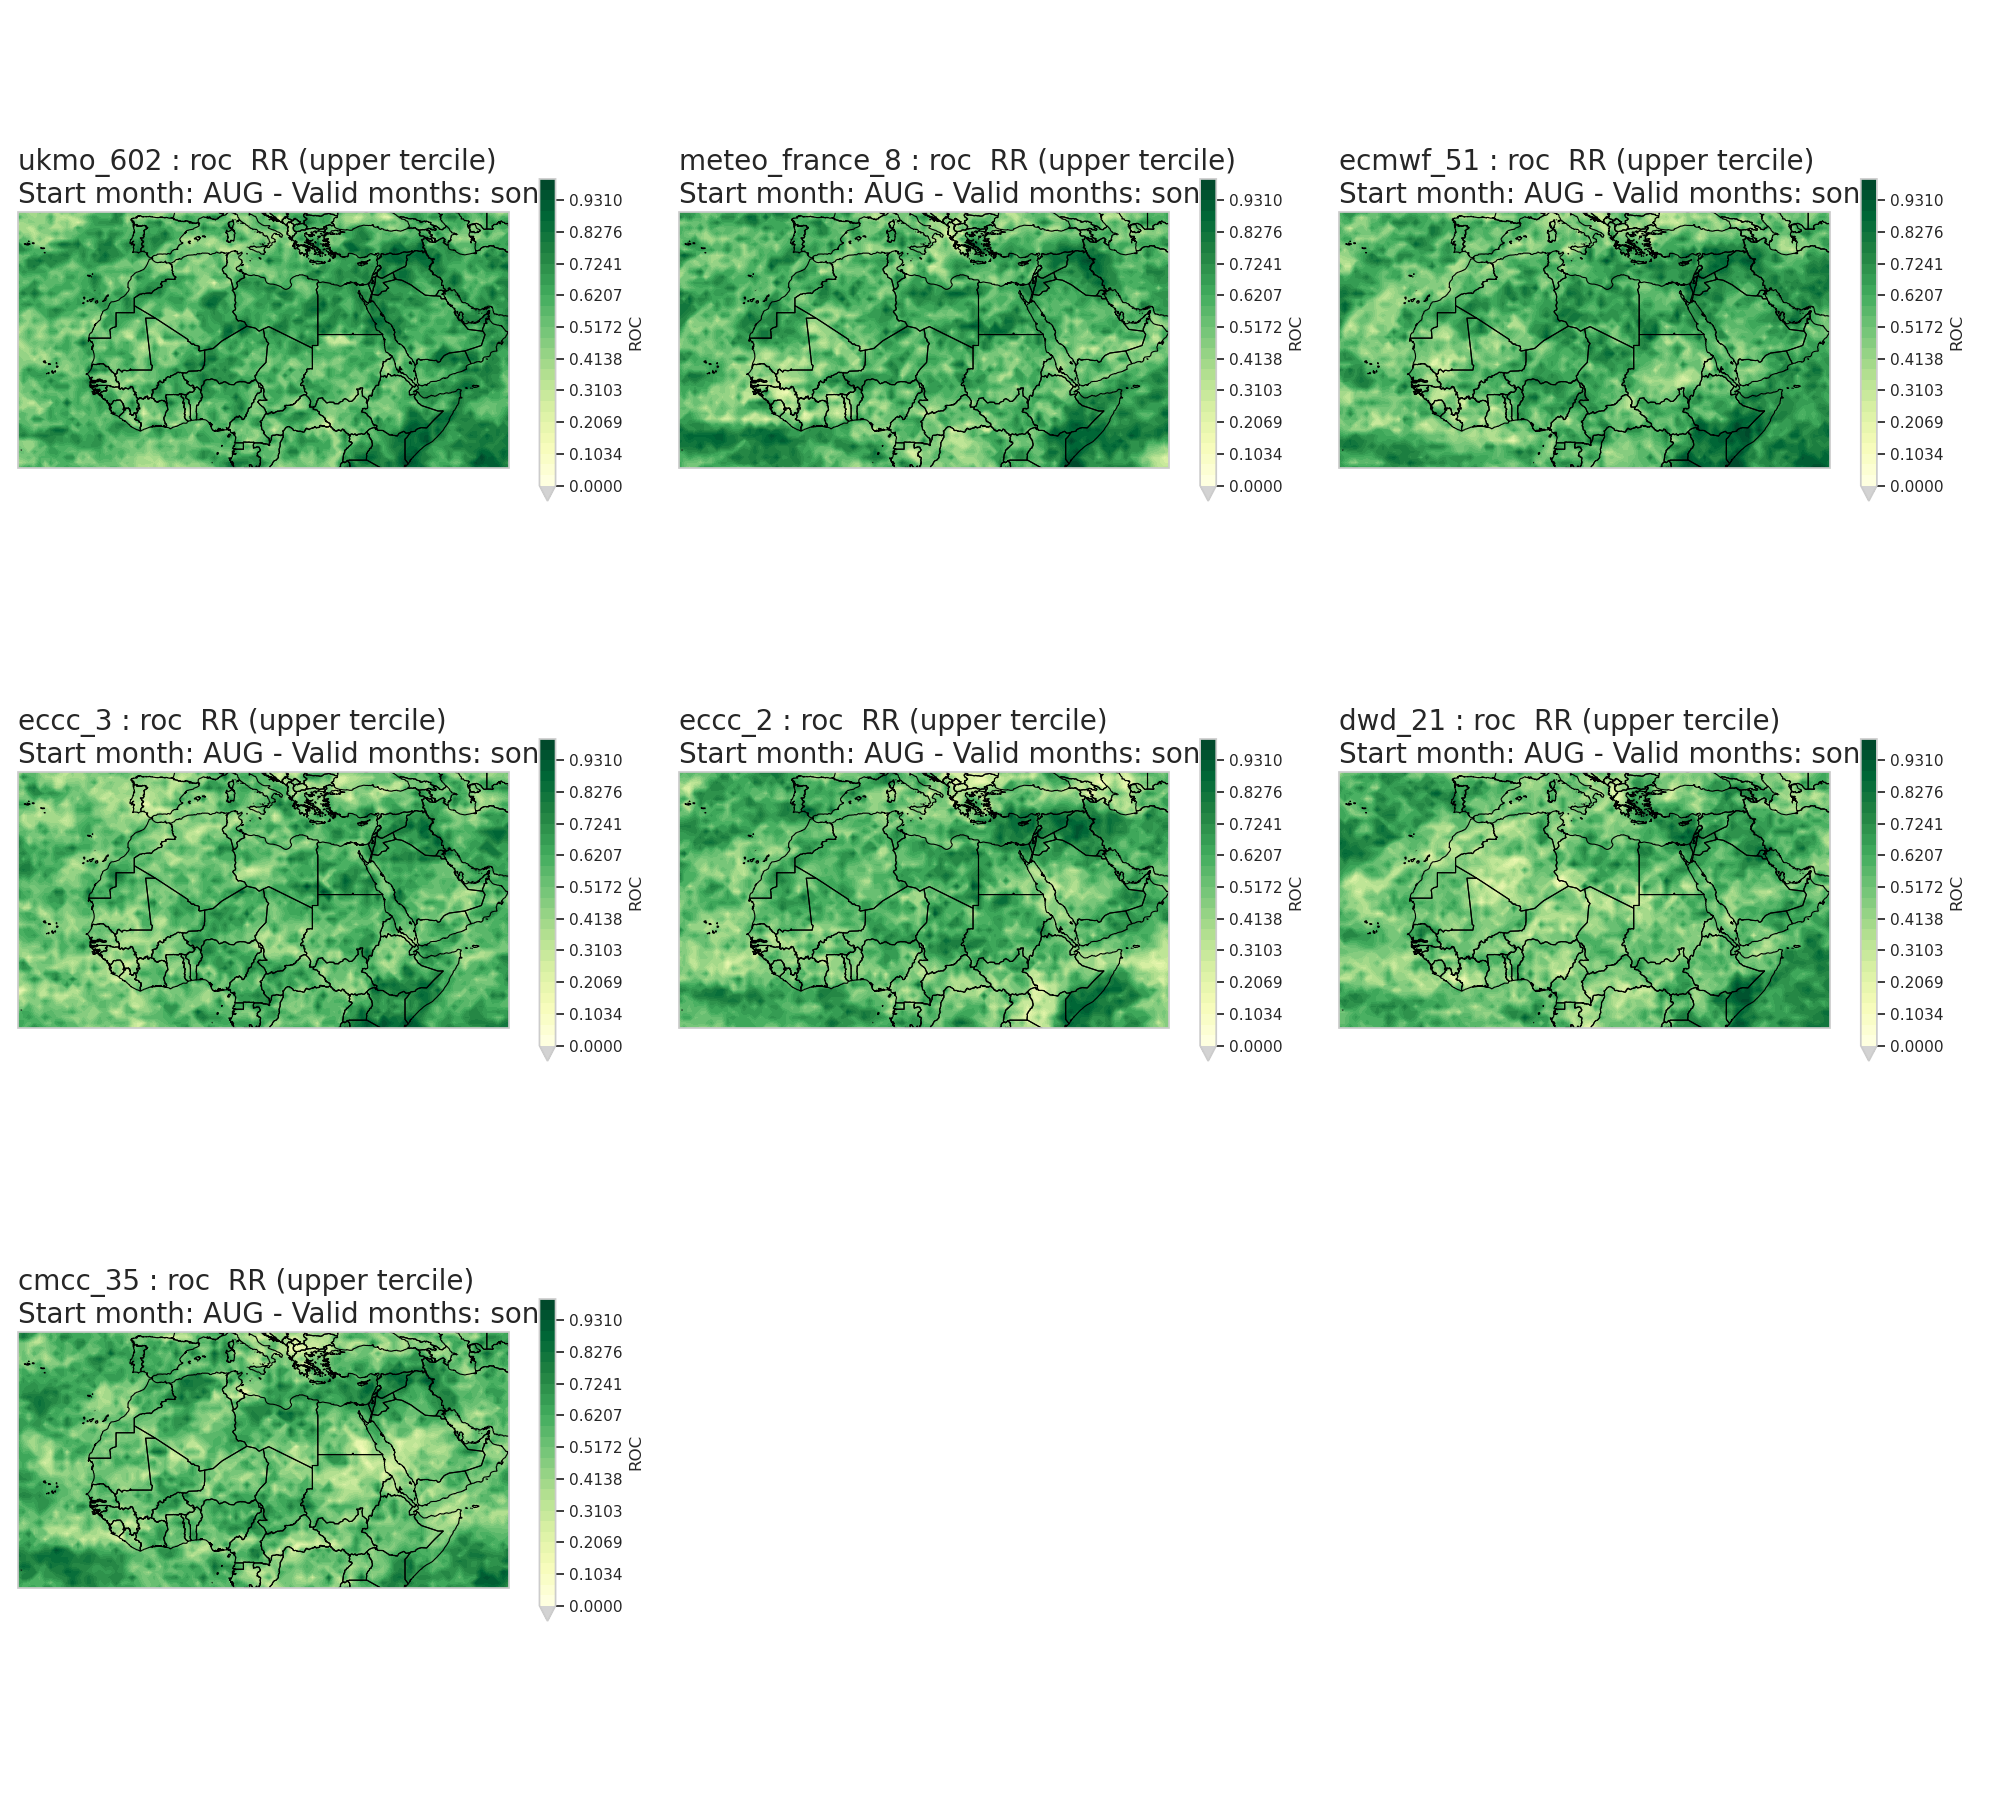
\includegraphics[scale=0.3]{plots/prob/roc/roc_son_RR_upper.png}
    \caption{The ROC Score Upper tercile SON    . \textbf{\textit{(1 means perfect ROC)}}}
\end{figure}

the spacial distribution of the roc score confirms an important result. For precipitation all centers shows better performance for the East of Africa, Irak,Syria,Jordan and Palestine. The performance in this zone is very high (score near to 1). For the rest of MENA region the performance is similar, with moderate to good score.


\subsubsection{Relative operating characteristics Skill Score}

In the figure above, the ECMWF exhibit the best performance for all terciles and periods. However, we should notice that the performance is very low for the middle tercile in all centers. For the analysis along time, the performance is so low, the best performance is in the first lead-time, except the SON which shows the best performance for the second lead-time. Above all, the \textbf{\textit{ecmwf}} shows the best performance.

\begin{figure}[H]
    \centering
    \includegraphics[scale=0.25]{plots/prob/rocss/rocss_RR_category.png}
    \caption{The ROCSS Score for each category  . \textbf{\textit{(1 means perfect ROCSS)}}}
\end{figure}


\begin{figure}[H]
    \centering
    \includegraphics[scale=0.25]{plots/prob/rocss/rocss_RR_lead_time.png}
    \caption{The average of  ROCSS Score on all categories    . \textbf{\textit{(1 means perfect ROCSS)}}}
\end{figure}



\begin{figure}[H]
    \centering
    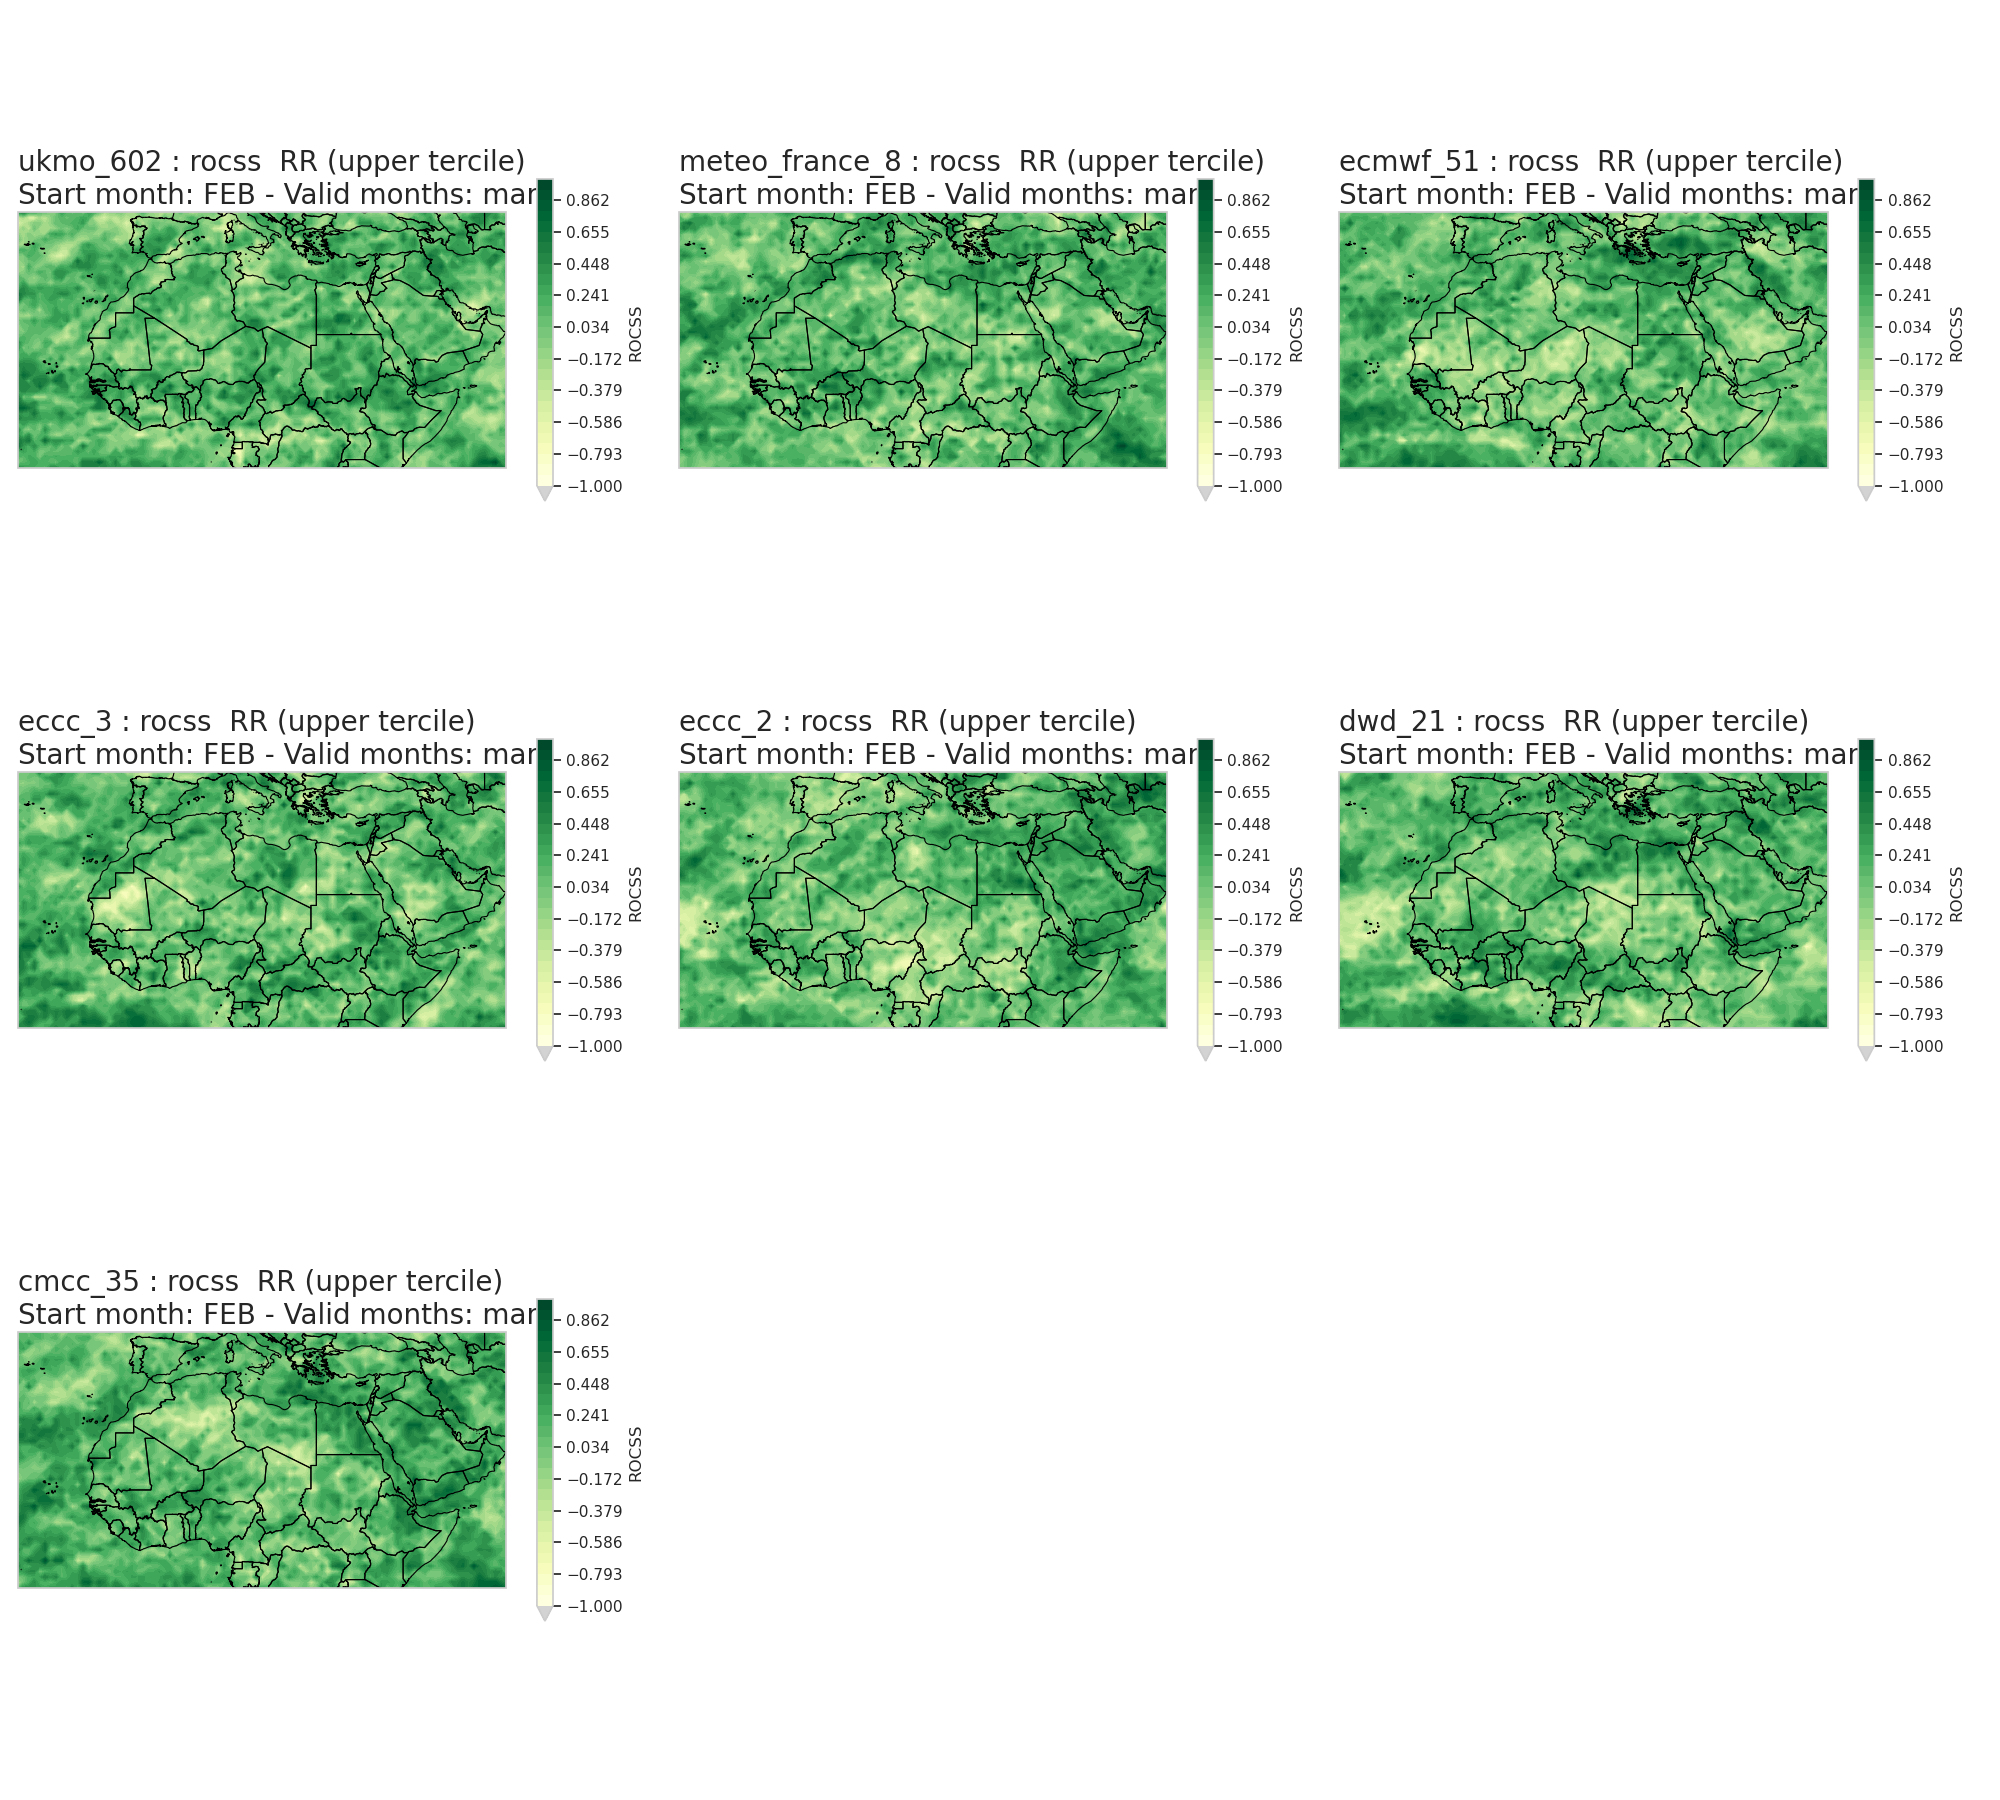
\includegraphics[scale=0.3]{plots/prob/rocss/rocss_mam_RR_upper.png}
    \caption{The ROC Skill Score Upper tercile MAM    . \textbf{\textit{(1 means perfect ROC)}}}
\end{figure}

the spacial distribution of the ROCSS, shows that all centers are consistent for this score. The spacial distribution isn't clear, there is a high spacial variability.








\subsubsection{summary}
\begin{table}[h!]
\centering
\begin{tabularx}{\textwidth}{@{}p{2.5cm}p{4cm}p{4cm}p{2.5cm}p{3cm}@{}}
\toprule
\textbf{Metric}       & \textbf{Focus}                                    & \textbf{What it Measures}                         & \textbf{Dependent on Observed Outcomes?} & \textbf{Visualization/Tools}             \\ \midrule
\textbf{Reliability}   & Probabilities match observed frequencies          & Calibration of probabilities                      & Yes                                      & Reliability diagram                      \\
\textbf{Discrimination} & Differentiating between outcomes                 & Ability to distinguish events from non-events    & Yes                                      & ROC curve, AUC                           \\
\textbf{Sharpness}     & Boldness of probabilities (away from average)     & Confidence of the forecast                        & No                                       & Histogram of forecast probabilities      \\
\textbf{Resolution}    & Informativeness and variability of forecast       & Ability to provide specific, useful info         & Yes                                      & Brier Score decomposition                \\ \bottomrule
\end{tabularx}
\caption{Key differences between reliability, discrimination, sharpness, and resolution in seasonal forecasting.}
\label{tab:forecast_metrics}
\end{table}

\newpage
\thispagestyle{empty}
\mbox{}

\endinput

